% Generated fragments require trusted human review before compilation.
% This binder never requests shell escape or runs external tools.
\documentclass[11pt]{article}
% Trusted shared apparatus. Requires LuaLaTeX; never use shell escape.
\usepackage{fontspec}
\defaultfontfeatures{Ligatures=TeX}
\IfFontExistsTF{Noto Serif}{\setmainfont{Noto Serif}}{%
  \IfFontExistsTF{DejaVu Serif}{\setmainfont{DejaVu Serif}}{%
    \IfFontExistsTF{Times New Roman}{\setmainfont{Times New Roman}}{%
      \PackageError{gelfand-binder}{No configured Cyrillic serif font installed}{Install Noto Serif or DejaVu Serif, or select an installed Cyrillic font.}%
    }%
  }%
}
\IfFontExistsTF{Noto Sans}{\setsansfont{Noto Sans}}{%
  \IfFontExistsTF{DejaVu Sans}{\setsansfont{DejaVu Sans}}{\setsansfont{Arial}}%
}
\IfFontExistsTF{Noto Sans Mono}{\setmonofont{Noto Sans Mono}}{%
  \IfFontExistsTF{DejaVu Sans Mono}{\setmonofont{DejaVu Sans Mono}}{\setmonofont{Courier New}}%
}
\usepackage[a4paper,margin=22mm]{geometry}
\usepackage{amsmath,amssymb,amsthm,mathtools}
\usepackage{xcolor}
\usepackage{tikz}
\usepackage{tikz-cd}
\usetikzlibrary{arrows.meta,positioning,calc}
\usepackage{hyperref}
\hypersetup{unicode=true,colorlinks=true,linkcolor=blue,pdftitle={Gelfand transcription binder}}
\newtheorem{theorem}{Theorem}
\newtheorem{lemma}{Lemma}
\newtheorem{proposition}{Proposition}
\newtheorem{corollary}{Corollary}
\theoremstyle{definition}
\newtheorem{definition}{Definition}
\newtheorem{example}{Example}
\theoremstyle{remark}
\newtheorem{remark}{Remark}
\setlength{\parindent}{0pt}
\setlength{\parskip}{0.55em}
\setlength{\emergencystretch}{3em}
\newcommand{\SourcePage}[2]{%
  \clearpage\phantomsection\label{#1:source-page}%
  \addcontentsline{toc}{subsection}{#1}%
  {\small\sffamily\color{blue!60!black}Source scan frame: #1; visible page/leaf label: #2}\par\medskip%
}
\newcommand{\Unclear}[3]{%
  \begingroup\color{orange!70!black}%
  [Unresolved reading #1/#2: #3]\endgroup%
}
\newcommand{\Incomplete}[3]{%
  \par\begingroup\color{red!65!black}\textbf{Incomplete #1/#2:} #3\endgroup\par%
}
\newcommand{\SourceFigure}[3]{%
  \par\begingroup\color{blue!60!black}\textbf{\hyperref[#1:source-page]{Source figure #1/#2}:} #3%
  \par\textit{Consult the authoritative scan at this locator.}\endgroup\par%
}



% Reader layout only. Original diplomatic text is retained verbatim.
\setlength{\parskip}{0.35em}
\setlength{\emergencystretch}{4em}
\renewcommand{\SourcePage}[2]{%
  \par\addvspace{1em}\phantomsection\label{#1:source-page}%
  \addcontentsline{toc}{subsection}{#1}%
  {\footnotesize\sffamily\color{blue!55!black}#1%
    \def\givenlabel{#2}\def\nolabel{unlabelled}%
    \ifx\givenlabel\nolabel\else\quad[номер в источнике: #2]\fi
  }\par\nobreak\smallskip%
}
\renewcommand{\Unclear}[3]{%
  \begingroup\color{orange!65!black}%
  \ifmmode\text{[неясно: #3]}\else[неясно: #3]\fi\endgroup%
}
\renewcommand{\Incomplete}[3]{%
  \par\begingroup\color{red!60!black}\textbf{Неразобранный фрагмент:} #3%
  \endgroup\par%
}
\renewcommand{\SourceFigure}[3]{%
  \par\begingroup\color{blue!55!black}\textbf{Рисунок:} #3%
  \par{\small\textit{Исходный рисунок: \hyperref[#1:source-page]{#1}, #2.}}%
  \endgroup\par%
}
\hypersetup{pdftitle={Семинар И. М. Гельфанда. Дипломатическая транскрипция},pdfauthor={},pdfsubject={Русское рабочее издание с отмеченными сомнительными чтениями}}

\usepackage[normalem]{ulem}
\usepackage{newunicodechar}
\usepackage{adjustbox}
\newfontfamily\SourceSymbolFont{Segoe UI Symbol}
\newfontfamily\SourceCJKFont{MS Gothic}
\let\DiplomaticMathUnderline\underline
\renewcommand{\underline}[1]{\ifmmode\DiplomaticMathUnderline{#1}\else\uline{#1}\fi}
\newunicodechar{→}{\ifmmode\text{{\SourceSymbolFont\char"2192}}\else{\SourceSymbolFont\char"2192}\fi}
\newunicodechar{⇒}{\ifmmode\text{{\SourceSymbolFont\char"21D2}}\else{\SourceSymbolFont\char"21D2}\fi}
\newunicodechar{∀}{\ifmmode\text{{\SourceSymbolFont\char"2200}}\else{\SourceSymbolFont\char"2200}\fi}
\newunicodechar{∂}{\ifmmode\text{{\SourceSymbolFont\char"2202}}\else{\SourceSymbolFont\char"2202}\fi}
\newunicodechar{∈}{\ifmmode\text{{\SourceSymbolFont\char"2208}}\else{\SourceSymbolFont\char"2208}\fi}
\newunicodechar{∌}{\ifmmode\text{{\SourceSymbolFont\char"220C}}\else{\SourceSymbolFont\char"220C}\fi}
\newunicodechar{√}{\ifmmode\text{{\SourceSymbolFont\char"221A}}\else{\SourceSymbolFont\char"221A}\fi}
\newunicodechar{∞}{\ifmmode\text{{\SourceSymbolFont\char"221E}}\else{\SourceSymbolFont\char"221E}\fi}
\newunicodechar{∧}{\ifmmode\text{{\SourceSymbolFont\char"2227}}\else{\SourceSymbolFont\char"2227}\fi}
\newunicodechar{∩}{\ifmmode\text{{\SourceSymbolFont\char"2229}}\else{\SourceSymbolFont\char"2229}\fi}
\newunicodechar{∪}{\ifmmode\text{{\SourceSymbolFont\char"222A}}\else{\SourceSymbolFont\char"222A}\fi}
\newunicodechar{∫}{\ifmmode\text{{\SourceSymbolFont\char"222B}}\else{\SourceSymbolFont\char"222B}\fi}
\newunicodechar{∴}{\ifmmode\text{{\SourceSymbolFont\char"2234}}\else{\SourceSymbolFont\char"2234}\fi}
\newunicodechar{∼}{\ifmmode\text{{\SourceSymbolFont\char"223C}}\else{\SourceSymbolFont\char"223C}\fi}
\newunicodechar{≈}{\ifmmode\text{{\SourceSymbolFont\char"2248}}\else{\SourceSymbolFont\char"2248}\fi}
\newunicodechar{≠}{\ifmmode\text{{\SourceSymbolFont\char"2260}}\else{\SourceSymbolFont\char"2260}\fi}
\newunicodechar{≤}{\ifmmode\text{{\SourceSymbolFont\char"2264}}\else{\SourceSymbolFont\char"2264}\fi}
\newunicodechar{≥}{\ifmmode\text{{\SourceSymbolFont\char"2265}}\else{\SourceSymbolFont\char"2265}\fi}
\newunicodechar{⊕}{\ifmmode\text{{\SourceSymbolFont\char"2295}}\else{\SourceSymbolFont\char"2295}\fi}
\newunicodechar{⊗}{\ifmmode\text{{\SourceSymbolFont\char"2297}}\else{\SourceSymbolFont\char"2297}\fi}
\newunicodechar{①}{\ifmmode\text{{\SourceSymbolFont\char"2460}}\else{\SourceSymbolFont\char"2460}\fi}
\newunicodechar{②}{\ifmmode\text{{\SourceSymbolFont\char"2461}}\else{\SourceSymbolFont\char"2461}\fi}
\newunicodechar{③}{\ifmmode\text{{\SourceSymbolFont\char"2462}}\else{\SourceSymbolFont\char"2462}\fi}
\newunicodechar{④}{\ifmmode\text{{\SourceSymbolFont\char"2463}}\else{\SourceSymbolFont\char"2463}\fi}
\newunicodechar{Ⓗ}{\ifmmode\text{{\SourceSymbolFont\char"24BD}}\else{\SourceSymbolFont\char"24BD}\fi}
\newunicodechar{〃}{\ifmmode\text{{\SourceCJKFont\char"3003}}\else{\SourceCJKFont\char"3003}\fi}


% Reader revision 3. Annotation wording and candidates remain unchanged.
\setmainfont{NotoSerif-Regular.ttf}[Path=C:/Windows/Fonts/,ItalicFont=NotoSerif-Italic.ttf,BoldFont=NotoSerif-Bold.ttf,BoldItalicFont=NotoSerif-BoldItalic.ttf]
\usetikzlibrary{shapes.geometric,decorations.pathreplacing,decorations.markings,patterns,fit}
\newsavebox{\ReaderAnnotationBox}
\newcommand{\ReaderAnnotation}[1]{%
  \sbox{\ReaderAnnotationBox}{[неясно: #1]}%
  \ifdim\wd\ReaderAnnotationBox>.70\linewidth
    \parbox[t]{.70\linewidth}{\raggedright[неясно: #1]}%
  \else\usebox{\ReaderAnnotationBox}\fi%
}
\ExplSyntaxOn
\cs_new_protected:Npn \reader_unclear_candidate:n #1
 {
  \tl_set:Nx \l_tmpa_tl { \tl_to_str:n {#1} }
  % Text explicitly guarded inside a mathematical candidate remains math-safe.
  \regex_replace_all:nnN { \\(?:text|textrm|textnormal|textbf|operatorname)\s*\{[^{}]*\} } { } \l_tmpa_tl
  \regex_match:nVTF { [\x{0400}-\x{052F}] | \$ } \l_tmpa_tl
   { \ifmmode \text{\ReaderAnnotation{#1}} \else \ReaderAnnotation{#1} \fi }
   {
    \ifmmode
      \mathord{\underset{\text{\tiny неясно}}{#1}}
    \else
      \regex_match:nVTF { [_^] | \\ } \l_tmpa_tl
       { \ensuremath{[\text{неясно:~}#1]} }
       { \ReaderAnnotation{#1} }
    \fi
   }
 }
\RenewDocumentCommand \Unclear { m m m }
 { \begingroup\color{orange!65!black}\reader_unclear_candidate:n{#3}\endgroup }
\ExplSyntaxOff
\newsavebox{\ReaderIncompleteBox}
\newcommand{\ReaderApparatusRef}[2]{%
 \begingroup\ifnum#2=1\color{orange!65!black}\else\color{red!60!black}\fi%
 \ifmmode\text{\scriptsize[прим.\,#1]}\else{\scriptsize[прим.\,#1]}\fi\endgroup%
}
\newcommand{\ReaderNotesStart}[1]{%
 \par\addvspace{.4em}\begingroup\small%
 \textbf{Примечания к кадру #1.}\par%
}
\newcommand{\ReaderNote}[2]{\par\noindent[#1]\quad#2\par}
\newcommand{\ReaderNotesEnd}{\endgroup\par\addvspace{.4em}}
\newcommand{\ReaderIncompleteNote}[1]{%
 \sbox{\ReaderIncompleteBox}{\textbf{Неразобранный фрагмент:} #1}%
 \ifdim\wd\ReaderIncompleteBox>.70\linewidth
  \parbox[t]{.70\linewidth}{\raggedright\textbf{Неразобранный фрагмент:} #1}%
 \else\usebox{\ReaderIncompleteBox}\fi%
}
\renewcommand{\Incomplete}[3]{%
 \ifmmode\text{\color{red!60!black}\ReaderIncompleteNote{#3}}%
 \else\leavevmode\begingroup\color{red!60!black}\ReaderIncompleteNote{#3}\endgroup\fi%
}
% Ragged right avoids stretching long untranslated abbreviations into margins.
\AtBeginDocument{\raggedright}
\newunicodechar{А}{\ifmmode\text{\char"410\relax}\else\char"410\relax\fi}
\newunicodechar{Б}{\ifmmode\text{\char"411\relax}\else\char"411\relax\fi}
\newunicodechar{В}{\ifmmode\text{\char"412\relax}\else\char"412\relax\fi}
\newunicodechar{Г}{\ifmmode\text{\char"413\relax}\else\char"413\relax\fi}
\newunicodechar{Д}{\ifmmode\text{\char"414\relax}\else\char"414\relax\fi}
\newunicodechar{Е}{\ifmmode\text{\char"415\relax}\else\char"415\relax\fi}
\newunicodechar{Ж}{\ifmmode\text{\char"416\relax}\else\char"416\relax\fi}
\newunicodechar{З}{\ifmmode\text{\char"417\relax}\else\char"417\relax\fi}
\newunicodechar{И}{\ifmmode\text{\char"418\relax}\else\char"418\relax\fi}
\newunicodechar{Й}{\ifmmode\text{\char"419\relax}\else\char"419\relax\fi}
\newunicodechar{К}{\ifmmode\text{\char"41A\relax}\else\char"41A\relax\fi}
\newunicodechar{Л}{\ifmmode\text{\char"41B\relax}\else\char"41B\relax\fi}
\newunicodechar{М}{\ifmmode\text{\char"41C\relax}\else\char"41C\relax\fi}
\newunicodechar{Н}{\ifmmode\text{\char"41D\relax}\else\char"41D\relax\fi}
\newunicodechar{О}{\ifmmode\text{\char"41E\relax}\else\char"41E\relax\fi}
\newunicodechar{П}{\ifmmode\text{\char"41F\relax}\else\char"41F\relax\fi}
\newunicodechar{Р}{\ifmmode\text{\char"420\relax}\else\char"420\relax\fi}
\newunicodechar{С}{\ifmmode\text{\char"421\relax}\else\char"421\relax\fi}
\newunicodechar{Т}{\ifmmode\text{\char"422\relax}\else\char"422\relax\fi}
\newunicodechar{У}{\ifmmode\text{\char"423\relax}\else\char"423\relax\fi}
\newunicodechar{Ф}{\ifmmode\text{\char"424\relax}\else\char"424\relax\fi}
\newunicodechar{Х}{\ifmmode\text{\char"425\relax}\else\char"425\relax\fi}
\newunicodechar{Ц}{\ifmmode\text{\char"426\relax}\else\char"426\relax\fi}
\newunicodechar{Ч}{\ifmmode\text{\char"427\relax}\else\char"427\relax\fi}
\newunicodechar{Ш}{\ifmmode\text{\char"428\relax}\else\char"428\relax\fi}
\newunicodechar{Щ}{\ifmmode\text{\char"429\relax}\else\char"429\relax\fi}
\newunicodechar{Ъ}{\ifmmode\text{\char"42A\relax}\else\char"42A\relax\fi}
\newunicodechar{Ы}{\ifmmode\text{\char"42B\relax}\else\char"42B\relax\fi}
\newunicodechar{Ь}{\ifmmode\text{\char"42C\relax}\else\char"42C\relax\fi}
\newunicodechar{Э}{\ifmmode\text{\char"42D\relax}\else\char"42D\relax\fi}
\newunicodechar{Ю}{\ifmmode\text{\char"42E\relax}\else\char"42E\relax\fi}
\newunicodechar{Я}{\ifmmode\text{\char"42F\relax}\else\char"42F\relax\fi}
\newunicodechar{а}{\ifmmode\text{\char"430\relax}\else\char"430\relax\fi}
\newunicodechar{б}{\ifmmode\text{\char"431\relax}\else\char"431\relax\fi}
\newunicodechar{в}{\ifmmode\text{\char"432\relax}\else\char"432\relax\fi}
\newunicodechar{г}{\ifmmode\text{\char"433\relax}\else\char"433\relax\fi}
\newunicodechar{д}{\ifmmode\text{\char"434\relax}\else\char"434\relax\fi}
\newunicodechar{е}{\ifmmode\text{\char"435\relax}\else\char"435\relax\fi}
\newunicodechar{ж}{\ifmmode\text{\char"436\relax}\else\char"436\relax\fi}
\newunicodechar{з}{\ifmmode\text{\char"437\relax}\else\char"437\relax\fi}
\newunicodechar{и}{\ifmmode\text{\char"438\relax}\else\char"438\relax\fi}
\newunicodechar{й}{\ifmmode\text{\char"439\relax}\else\char"439\relax\fi}
\newunicodechar{к}{\ifmmode\text{\char"43A\relax}\else\char"43A\relax\fi}
\newunicodechar{л}{\ifmmode\text{\char"43B\relax}\else\char"43B\relax\fi}
\newunicodechar{м}{\ifmmode\text{\char"43C\relax}\else\char"43C\relax\fi}
\newunicodechar{н}{\ifmmode\text{\char"43D\relax}\else\char"43D\relax\fi}
\newunicodechar{о}{\ifmmode\text{\char"43E\relax}\else\char"43E\relax\fi}
\newunicodechar{п}{\ifmmode\text{\char"43F\relax}\else\char"43F\relax\fi}
\newunicodechar{р}{\ifmmode\text{\char"440\relax}\else\char"440\relax\fi}
\newunicodechar{с}{\ifmmode\text{\char"441\relax}\else\char"441\relax\fi}
\newunicodechar{т}{\ifmmode\text{\char"442\relax}\else\char"442\relax\fi}
\newunicodechar{у}{\ifmmode\text{\char"443\relax}\else\char"443\relax\fi}
\newunicodechar{ф}{\ifmmode\text{\char"444\relax}\else\char"444\relax\fi}
\newunicodechar{х}{\ifmmode\text{\char"445\relax}\else\char"445\relax\fi}
\newunicodechar{ц}{\ifmmode\text{\char"446\relax}\else\char"446\relax\fi}
\newunicodechar{ч}{\ifmmode\text{\char"447\relax}\else\char"447\relax\fi}
\newunicodechar{ш}{\ifmmode\text{\char"448\relax}\else\char"448\relax\fi}
\newunicodechar{щ}{\ifmmode\text{\char"449\relax}\else\char"449\relax\fi}
\newunicodechar{ъ}{\ifmmode\text{\char"44A\relax}\else\char"44A\relax\fi}
\newunicodechar{ы}{\ifmmode\text{\char"44B\relax}\else\char"44B\relax\fi}
\newunicodechar{ь}{\ifmmode\text{\char"44C\relax}\else\char"44C\relax\fi}
\newunicodechar{э}{\ifmmode\text{\char"44D\relax}\else\char"44D\relax\fi}
\newunicodechar{ю}{\ifmmode\text{\char"44E\relax}\else\char"44E\relax\fi}
\newunicodechar{я}{\ifmmode\text{\char"44F\relax}\else\char"44F\relax\fi}
\newunicodechar{Ё}{\ifmmode\text{\char"401\relax}\else\char"401\relax\fi}
\newunicodechar{ё}{\ifmmode\text{\char"451\relax}\else\char"451\relax\fi}

\newunicodechar{æ}{\ifmmode\text{\char"E6\relax}\else\char"E6\relax\fi}
\newunicodechar{−}{\ifmmode\mathbin{\text{\SourceSymbolFont\char"2212\relax}}\else{\SourceSymbolFont\char"2212\relax}\fi}


% Reader-only pairing support; accepted raw bodies remain unchanged.
\RequirePackage{graphicx}
\RequirePackage{adjustbox}
\newcommand{\ReaderOriginalPanel}[2]{%
  \begin{minipage}[t]{.48\linewidth}\vspace{0pt}\centering
    \includegraphics[width=\linewidth,keepaspectratio]{#1}\par\smallskip
    {\scriptsize Оригинал рукописного рисунка: #2}\par
  \end{minipage}%
}
\newcommand{\ReaderDiagramPair}[3]{%
  \par\noindent\begingroup
  \ReaderOriginalPanel{#1}{#2}\hfill
  \begin{minipage}[t]{.48\linewidth}\vspace{0pt}\centering
    {\scriptsize Типографское воссоздание}\par\smallskip
    \begin{adjustbox}{max width=\linewidth}#3\end{adjustbox}\par
  \end{minipage}%
  \endgroup\par\smallskip
}
\newcommand{\ReaderDescriptionPair}[3]{%
  \par\noindent\begingroup
  \ReaderOriginalPanel{#1}{#2}\hfill
  \begin{minipage}[t]{.48\linewidth}\vspace{0pt}\raggedright
    {\scriptsize Типографское описание}\par\smallskip
    #3\par
  \end{minipage}%
  \endgroup\par\smallskip
}


\begin{document}
\begin{center}
{\Large Семинар И. М. Гельфанда}\par\medskip
{\LARGE Дипломатическая транскрипция}\par\bigskip
{\large Рабочее русское издание}\par\medskip
{\large Том 07 из 34. Архивная глава 007}\par\bigskip
Кадры GELFAND-P000501 -- GELFAND-P000553\par
\end{center}
\medskip
Сокращения, отменённые записи и сомнительные чтения сохранены.
Неразобранные фрагменты отмечены в тексте. Математические утверждения
источника переданы без молчаливых исправлений.

В текущем комплекте приняты 165 из 165 возвратов; учтены 1527 из 1527 кадров. Кадров без принятого возврата: 0.
Статусы кадров в отчётах о полноте: транскрибированы 1168, неразборчивы 357, частично прочитаны 1, недоступны 1.
Нерешённых записей журнала чтений: 6820.
Статус «неразборчивый» может отмечать локальную утрату зачёркнутой записи;
он не означает отсутствия всего кадра.
Сверка с рукописью продолжается. Рабочие журналы чтений и происхождения
данных сохранены отдельно.

Ограничения исходного комплекта: повреждённый исходный скан GELFAND-P000722; каталожные записи 603, 694 без сканов; в архивной главе 029 не перечислена часть 25.

Границы кадров показаны небольшими синими указателями; печатный текст
продолжается без обязательного разрыва страницы после каждого кадра.
\bigskip\hrule\bigskip
\SourcePage{GELFAND-P000501}{1}
\underline{3/IX-73.}\qquad
\underline{Сем.} [Зачёркнуто: \Incomplete{GELFAND-P000501}{heading-cancelled}{Текст густо затёрт; чтение не восстановлено.}] \underline{Гельфанда.}

\underline{План:}

1. Производная категория (Кириллов, Бернштейн).

2. Теория Алфорса — Неванлинна для многих переменных (и Грауэрту).
(Хенкин, Шабат).

3. $K$-теория (\Unclear{GELFAND-P000501}{plan-k-theory}{симплициальный вариант}) по Quillen'у (Фукс).

4. Гипотеза Лихтенбаума о связи между $\zeta$-ф-ей в целых точках
и высшими $K$-теориями (Манин).

5. Вей: идеология \Unclear{GELFAND-P000501}{plan-item-five}{Герстенцуса}.

[Слева зачёркнут номер: \Unclear{GELFAND-P000501}{interlude-number}{6 или 8}.]
\underline{Интермедия:}
\underline{2 проблемы Серра:}

1) $k[t]$, $k$ — конечно;
$SL_n(k[t])$, $n\geq 3$;
$SL_n(k[t,t^{-1}])$, $n\geq 2$.

Эти группы имеют конечное число образующих. Являются ли они
конечно представленными? (Сущ. ли образ., между котор. конечное
число соотнош.)

2) Когер. группа: $\forall$ подгр. с кон. числом обр. конечно представлена.
Свободная и \Unclear{GELFAND-P000501}{coherent-groups}{плоск.} когерентны.
Фунд. группы 3-мерных мн-зий когерентны
(G. P. Scott, J. Lond. Math. Soc., (2)6 (1973), 437--440). Статья.
$SL_2(\Lambda)$ когер., где $\Lambda$ —
\Unclear{GELFAND-P000501}{lambda-description}{чисто мнимые элем. квадр. поля}.
[Зачёркнуто: \Unclear{GELFAND-P000501}{lambda-cancelled}{ещё}.]

Явл. ли $SL_3(\mathbb{Z})$ или $SL_2(\mathbb{Z}[\frac1p])$ когерентными?
$GL_n(\mathbb{Q})$?

[Много ли \Unclear{GELFAND-P000501}{interlude-relations}{соотн.} между разл. \Unclear{GELFAND-P000501}{interlude-question}{неприводимыми}? (кон. чис-лом)]

[Какие бывают фун. группы?]

6. \underline{Смейл:} оптимизация нескольких функций.

7. \underline{Браун, Дуглас, Филлмор}
Правильная $K$-теория от нескольких переменных (Кириллов).

8. \underline{Мищенко:} представления в его смысле.

9. \underline{\Unclear{GELFAND-P000501}{novikov-name}{Люстиг}}:
высш. сигн. Новикова.\qquad J. Diff. Geom. 197(1)

10. \underline{Атия, Ботт, Патоди об $L$-функциях, связ. с ур-ями.}
(спектр. асимметр. и т. д.) (Шубин)

11. \underline{Донован, Фрейлих}
\Unclear{GELFAND-P000501}{plan-item-eleven-mark}{а}
(В. Пономарёв) — четвёрки подпр-в и т. д.
Модули и т. д.

12. Ю. И. Манин.

13. Вершик, Гельфанд, Граев — 6 вариаций на тему $SL_2$.

\underline{Ю. И. Манин.}\qquad \underline{$p$-адические меры}

\underline{Сюжет:} $\mathbb{Q}_p$;\quad $K$ — конечн. расш.
$X$ — компактное $p$-ад. аналит. мн-зие над $K$.
Пример: целые числа в $K$, их прямые произв. и т. п.

\begin{equation*}
\begin{gathered}
L\\
\vert\\
K\\
\vert\\
\mathbb{Q}_p
\end{gathered}
\qquad
\begin{gathered}
X\overset{f}{\longrightarrow}L\\
\text{аналит.}
\end{gathered}
\qquad
\text{целые }A\quad
\underline{\text{Прим.:}}\quad A\overset{x}{\longrightarrow}K
\quad\text{координата.}
\end{equation*}

\underline{Задача:} определить $\int f\,d\mu$, т. е. опр. разумн.
и \Unclear{GELFAND-P000501}{last-line-class}{интер.} класс мер $p$-адич. типа на $X$.

\SourcePage{GELFAND-P000502}{unlabelled}
\underline{Мотивировка:} а) есть $\zeta$-ф-и $L(s)$, $\mathbb{C}\longrightarrow\mathbb{C}$.
\begin{equation*}
\sum n^{-s};\qquad \sum\chi(n)n^{-s};\qquad \sum a_n n^{-s},
\quad\text{где }\sum a_n e^{2\pi i\lambda}\quad\text{автом. форма.}
\end{equation*}
\Unclear{GELFAND-P000502}{exponential-index}{В показателе после $2\pi i$ виден знак, похожий на $\lambda$.}

Для них класс инт. ф-л с адельным интегрированием
\begin{equation*}
L(\chi)=\int_{G_A/G_K}\chi\,d\mu.
\end{equation*}
\Unclear{GELFAND-P000502}{adele-quotient}{Знаменатель области интегрирования прочитан как $G_K$; петля под $G$ неясна.}
\Unclear{GELFAND-P000502}{adele-group-note}{$G_K$ — гл. адели.}

На самом деле аргумент — характер $L(\chi)$.

б) есть $p$-адич. аналоги $L(\chi)$ и $\zeta(s)$
(Леопольд — [Зачёркнуто: \Unclear{GELFAND-P000502}{cancelled-iwasawa}{Ивасава}.]
[Над строкой: Кубота]).
\begin{align*}
\zeta(2m)&=B_{2m}\frac{\pi^{2m}}{\ldots},\\
\zeta(1-2m)&=\,?\,\frac{B_{2m}}{2m},
\end{align*}
[Двойной вертикальный знак.]
(\Unclear{GELFAND-P000502}{sum-intro}{Г.}
$\displaystyle\sum_{n=1}^{\infty}n^3=\frac{B_4}{4}$

чётные и нечётные отличаются:
\begin{equation*}
-y''+p(x)y=\lambda y,\qquad \sum\lambda_n^k
\end{equation*}
отличаются целые и полуцелые)

Ещё неизв. почему такую $\sum n^3$ через $B$ выр.!)
\Unclear{GELFAND-P000502}{bernoulli-formulas}{Формулы с $B_{2m}/(2m)$ и $\sum n^3=B_4/4$ сохранены со знаками рукописи.}

Смысл след. плана — \Unclear{GELFAND-P000502}{kronecker-abbreviation}{пред.} ф-лы Кронекера.
Выбр. $p$ из эйл. произв.
\begin{equation*}
1-2m\longrightarrow\frac{B_{2m}}{2m}(1-p^{2m-1})\qquad\text{Фикс. }p!
\end{equation*}
$p$-адич. непр. и даже \Unclear{GELFAND-P000502}{analytic-ending}{аналитичне} !!!
[Зачёркнуто: \Unclear{GELFAND-P000502}{cancelled-euler-comment}{(убрали из эйл. произв. выб. $p$)}.]
[Последние две строки объединены снизу длинной скобкой.]

\begin{equation*}
\begin{gathered}
\zeta(s)(1-p^{-s})\\
\mathbb{C}\longrightarrow\mathbb{C}
\end{gathered}
\qquad\text{между.}\qquad
\begin{gathered}
\zeta^{(p)}(s_p)\\
\mathbb{Z}_p\longrightarrow\mathbb{Q}_p
\end{gathered}
\end{equation*}
есть пересечение $\mathbb{C}$ и $\mathbb{Z}_p$ (целые), там одни и те же знач.

\SourceFigure{GELFAND-P000502}{embedding-diagram}{Схема начинается с $\{1-2m\}=E\subset$;
далее два обозначения полей со знаком пересечения, справа $\mathbb{Q}_p$.
Над первым обозначением написано $\mathbb{C}$, к нему идёт короткая стрелка вверх;
над правым обозначением идёт стрелка вправо вверх к $\mathbb{Q}_p$.
Чтение первого нижнего обозначения и точное прикрепление короткой стрелки требуют сверки со сканом.}
и они аналитичны.

На самом деле, видимо, правильный аргумент — адельный.
\begin{equation*}
\mathbb{Q}_p\longrightarrow\mathbb{Q}_{\ell}\quad(p\ne\ell)\text{видимо, проще (но неизв.)}
\end{equation*}
Трудно $\mathbb{Q}_p\longrightarrow\mathbb{Q}_p$,

Начал \underline{Мазур}.

\underline{Меры на $p$-адич. компактных пр-вах.}

$K$ — конечн. расш. $\mathbb{Q}_p$;\quad $A$ — целые в $K$;
$A\supset\overline{m}$ (макс. идеал)
[Под $A$: (корни ур-й с целыми коэфф.)]
\begin{equation*}
\operatorname{Card}(A/\overline{m})\underset{\mathrm{def}}{=}q.
\end{equation*}
Комп. анал. мн-зие над $K$.
\begin{equation*}
A^n=\underbrace{A\times\ldots\times A}_{n}\quad\text{— $n$-мерный шар.}
\end{equation*}
\underline{Анал. мн-зие:} пр-во и пучок ф-й, лок. устр. — шар.

\underline{Теорема (Серр):} $X$ — комп. ан. мн-зие над $K$ разм. $n$. Тогда

а) $X\simeq rA^n$ (аналит. изом.), $r\in\mathbb{N}$.
\Unclear{GELFAND-P000502}{theorem-count}{Повторяющийся знак числа шаров прочитан как $r$; возможно $\tau$.}

\begin{center}
\begin{adjustbox}{max width=\linewidth}
\begin{tikzpicture}
\draw (0,0) ellipse (0.25 and 0.18);
\draw (1,0) ellipse (0.20 and 0.15);
\draw (1.8,0) ellipse (0.17 and 0.13);
\draw (2.6,0) ellipse (0.16 and 0.14);
\node at (5.6,0) {— непересек. шары};
\end{tikzpicture}
\end{adjustbox}
\end{center}

б) [Зачёркнуто: если.] $rA^n\simeq r'A^n\ \Leftrightarrow\ r\equiv r'\ \operatorname{mod}(q-1)$
[Знак $\Leftrightarrow$ обведён.]

\SourcePage{GELFAND-P000503}{2}
\begin{gather*}
A=\{a\in K\mid a\text{ целое}\}.\qquad
A=\bigcup_{a_i\ \mathrm{mod}\ m}\{a\equiv a_i\ \mathrm{mod}\ m\}.
\end{gather*}
\underline{Как вычислять $\Unclear{GELFAND-P000503}{invariant-letter}{r}$?}

\underline{Примеры:} а) $X$ — алг. мн-зие над $A$ (гладкая схема над $\operatorname{Spec}A$).

[Зачёркнуто: \Incomplete{GELFAND-P000503}{cancelled-question}{Начало читается «Как вычислять $r$», конец похож на «теор. Серре»; промежуточный текст не восстановлен.}]

Редукция $X_0\quad\underset{\text{над }\operatorname{Spec}A.}{\text{(замкн. слой)}}$
— алг. мн-зие на $A/\bar m$
\begin{gather*}
\operatorname{Card}X_0(A/\bar m)=r(X).
\end{gather*}
\underline{Пример} схемы: $X=P^1$ или окружность.\qquad
2 афф. прямые скл. $x=y^{-1}$

Редукция: проект. прям. над кон. полем из $q$ элем. — там $q+1$ элем.
\begin{gather*}
q+1=2\ \mathrm{mod}(q-1).
\end{gather*}
Итак 2 шара:
\SourceFigure{GELFAND-P000503}{two-balls}{Два отдельных округлых контура рядом. Верхняя часть левого контура густо зачернена; верхняя часть правого имеет разрыв и короткие угловые штрихи у разрыва. Справа от контуров написано «и» и нарисован маленький округлый знак.}
\begin{gather*}
P^1(K)=\mathbb Q_p\cup\infty,\qquad pA\cup A^{-1}.
\end{gather*}
б) $X$ — $p$-адич. комп. гр. Ли; она проконечна, у $\forall$ фактора есть порядок.

Порядок: $2^2\,3^\infty\,\Unclear{GELFAND-P000503}{supernatural-exponent}{5^{-1}}\,7^0\,11^\infty\ldots$ — сверхъестеств. число (т.к. делятся друг на друга).

Оказывается, $\operatorname{ord}X=p^\infty\cdot N$, где $(p,N)=1$, $N$ — обычн. целое.
\begin{gather*}
\underline{\underline{N=r(X)}}
\end{gather*}
\Unclear{GELFAND-P000503}{sl2-count}{$SL_2$ — $(p-1)$ шаров $(=p^2-1\ \mathrm{mod}\ p)$}

\SourceFigure{GELFAND-P000503}{margin-fields}{На левом поле буква $L$ над буквой $K$; между ними густо зачёркнутый или переписанный знак, исходная форма и направление которого не читаются.}
\underline{Определение:} $L$-мера на $X$ — это $L$-значная конечно-аддит. ф-я на открыто-замкн. подмн-вах $X$.

($X$ — комп. \Unclear{GELFAND-P000503}{definition-overwrite}{анал.} мн-зие).

\underline{Примеры:} а) $X=\mathbb Z_p$
\SourceFigure{GELFAND-P000503}{clopen-tree}{Вверху одна чёрная вершина с подписью $X$ справа. Из неё идут четыре линии вниз к четырём чёрным вершинам; под каждой расходится пучок коротких линий. Самая левая нижняя линия длиннее остальных и уходит влево вниз. В центральных пучках некоторые штрихи сливаются.}

Вершины — откр.-замкн. подмн-ва.

Последовательно строим эти меры. Получ. фунд. сист. окрестностей.
\begin{gather*}
\text{Мера на }X\leftrightarrow
\{\mu(a+(p^m))\in L;\quad a\ \mathrm{mod}(p^m),\ m\in\mathbb N\}.\\
\mu(a+(p^m))=\sum_{b\equiv a\ \mathrm{mod}\ p^m}\mu(b+(p^{m+1}))
\Unclear{GELFAND-P000503}{measure-braces}{\}}.
\end{gather*}
И это применимо к любому компактному подмн-зию.
\begin{gather*}
\text{б) }\mu(a+(p^m))=\underbrace{\mathrm{const}\cdot p^{-m}}_{\in L}
\text{ — \underline{\underline{инвар. меры.}}}
\end{gather*}
На $L$ есть метрика ($p$-ад. модуль).
\begin{gather*}
|\mathrm{const}\cdot p^{-m}|_L\to\infty\quad\text{при }m\to\infty.
\end{gather*}
Чем меньше мн-ва, тем больше мера!!

К нулю не может стремиться! Тогда из неархим. следовало бы, что мера всего равна 0.

Инвар. меры — плохие.

Самая слабо раст. — ограниченная.
\begin{gather*}
\text{в) }\Unclear{GELFAND-P000503}{measure-signs}{\mu(a+(p^m))=1\text{ при }a<p^m/2,\quad-1\text{ при }a>p^m/2}
\end{gather*}
\begin{flushright}
$\Vert$ нетрив. огранич. мера
\end{flushright}
$0<a<p^m$, \Unclear{GELFAND-P000503}{bottom-cancelled-glyph}{[зачёркнуто: неразборчиво]} $(a,p)=1$\quad мера на $\mathbb Z_p^*$.

\SourcePage{GELFAND-P000504}{unlabelled}
\underline{Упражнение:} пров. аддитивность. Происх. интерференция.

Интегр. по ней — $\zeta$-ф-и Леопольда-Куботы.

эту меру придумал Мазур.

\underline{Интегралы.}

$X$, $\mu$ — мера со знач. в $L$.
\begin{flushright}
\begin{adjustbox}{max width=\linewidth}
\begin{tikzcd}[row sep=small]
L \arrow[d] \\
K.
\end{tikzcd}
\end{adjustbox}
\end{flushright}
$X\overset f\longrightarrow L$, аналит. ф-я.
\begin{gather*}
\int_X f\,d\mu\\
R=\{(U_i),\quad\underset{\text{откр.-замкн.}}{U_i}\text{ — разбиение }X,\quad a_i\in U_i\}\\
S(f,R)=\sum f(a_i)\mu(U_i).\\
\int_X f\,d\mu=\lim_R S(f,R)\quad\text{если предел сущ. при измельчении}
\end{gather*}
\underline{Пример.}

$X=\mathbb Z_p$, $\mu$ — инвар. $(\mu(a+(p^m))=p^{-m})$,
$L=\mathbb Q_p$.

$f=1$ интегрируется

\underline{\underline{$f=x$}} — прост. непост.
\begin{gather*}
\int f\,d\mu\quad\text{не сущ.!}\\
R=\{0\le a\le p^m-1,\quad a\in U_a\equiv\{b\mid b\equiv a\ \mathrm{mod}\ p^m\}.
\end{gather*}
\Unclear{GELFAND-P000504}{partition-exponent-cancelled}{[после $m$ в показателе зачёркнуто: $-1$]}
\begin{gather*}
S(f,R)=\frac1{p^m}\underbrace{\sum_{a=0}^{p^m-1}a}_{\frac{(p^m-1)p^m}{2}}\longrightarrow-\frac12.
\end{gather*}
\Unclear{GELFAND-P000504}{sum-exponent-cancelled}{[после $m$ в показателе первого $p$ под скобкой зачёркнуто: $-1$]}

Но это не единств. пред. точка.
\begin{gather*}
R'=\{p^m\in U_0\quad\text{остальное как в }R\}.
\end{gather*}
\underline{Предел будет другой:} измен. ф-и на интервале $\approx$ мере интерв.

\underline{отсюда усл. на меру:} при измельчении отнош. меры к инвар. мере должно $\to0$ (это в случае $n=1$).

\underline{Теорема:} пусть $X$ одномерно над $\mathbb Q_p$

1) $\mu$ — мера на $X$ со знач. в $L$, \Unclear{GELFAND-P000504}{moderate-overwrite}{умеренно} растущая, т.е.
\begin{gather*}
U\to\underset{\text{точка}}{\bullet}\Longrightarrow
|\mu(U)/\mu_{\mathrm{inv}}(U)|_L\to0.
\end{gather*}
($\mu_{\mathrm{inv}}$ — обыч. инв. мер на $\mathbb Z_p$).

2) $f:X\to L$ уд. усл. Липшица с показ. 1

Тогда $\int f\,d\mu$ существует.
\begin{flushright}
$\Vert$ \underline{След. раз:} конкр. меры и модул. формы.
\end{flushright}

\SourcePage{GELFAND-P000505}{unlabelled}
\Unclear{GELFAND-P000505}{top-right-label}{[знак за правой рамкой: неразборчиво]}

\underline{10.9.73.}\qquad\underline{\underline{Сем. Гельфанда.}}

\underline{Манин}\quad\underline{(продолжение).}

$X$ — 1-мерное $p$-адич. пр-во;

$\mu$ — $K$-мера на $X$\qquad ($K$ — конечн. расш. $\mathbb Q_p$)

\underline{$f:X\to K$}.
\begin{gather*}
R:\quad\text{данные Римана: }\{X=\bigcup_{i=1}^n U_i
\Unclear{GELFAND-P000505}{riemann-cancelled-brace}{\text{[зачёркнуто: }\}\text{]}},\quad a_i\in U_i\}.\\
S(f,R)=\sum\mu(U_i)f(a_i).
\end{gather*}
\underline{Теорема:}

$\exists\int_X f\,d\mu$, если

а) $f$ липшицева с пок. 1

б) $(U\mapsto\text{точка})\Longrightarrow|\mu(U)/\mu_{\mathrm{inv}}(U)|\to0$.

\underline{Пример.} $X=\mathbb Z_p$;
\begin{gather*}
\mu(a+(p^m))=\begin{cases}
-1&\text{при }0\le a<p^m/2\\
+1&\text{при }p^m/2<a<p^m.
\end{cases}
\end{gather*}
\underline{Дерево откр.-замкн. подмн-в:}
\begin{center}
\begin{adjustbox}{max width=\linewidth}
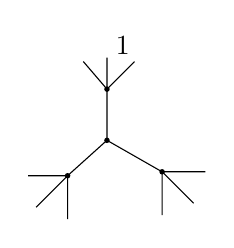
\begin{tikzpicture}[x=1cm,y=1cm]
\draw (0,0)--(-0.3,0.35) (0,0)--(0,0.4) (0,0)--(0.35,0.35);
\draw (0,0)--(0,-0.65) (0,-0.65)--(-0.5,-1.1) (0,-0.65)--(0.7,-1.05);
\draw (-0.5,-1.1)--(-1,-1.1) (-0.5,-1.1)--(-0.9,-1.5) (-0.5,-1.1)--(-0.5,-1.65);
\draw (0.7,-1.05)--(1.25,-1.05) (0.7,-1.05)--(1.1,-1.45) (0.7,-1.05)--(0.7,-1.6);
\fill (0,0) circle (0.035) (0,-0.65) circle (0.035) (-0.5,-1.1) circle (0.035) (0.7,-1.05) circle (0.035);
\node at (0.2,0.55) {$1$};
\end{tikzpicture}
\end{adjustbox}
\end{center}
$f(x)=x^{2\Unclear{GELFAND-P000505}{moment-index}{r}-1}$\qquad (для $f(x)=x^{2r}$ получится 0).
\begin{gather*}
\int_{\mathbb Z_p}x^{2r-1}d\mu=(-1)^r(1-2^{-r})\frac{B_{r-1}}{2r}.\\
\mathbb Z_p=\bigcup_{0\le a<\Unclear{GELFAND-P000505}{union-upper-bound}{p^{m-1}}}\{a+p^m\mathbb Z_p\}.
\end{gather*}
\Unclear{GELFAND-P000505}{margin-r}{$R$}
\begin{gather*}
S(f,R)=-\sum_{0\le a<p^m/2}a^{2r-1}+\sum_{p^m>a>p^m/2}a^{2r-1}.
\end{gather*}
Есть формулы Вороного, интерпретируемые как вычисление таких интегралов.
\begin{gather*}
\int_{\mathbb Z_p^*}=\int_{\mathbb Z_p}-\int_{p\mathbb Z_p}.\\
\int_{\mathbb Z_p^*}x^{2r-1}d\mu
=\Unclear{GELFAND-P000505}{lower-powers}{(1-p^{2m-1})}\int_{\Unclear{GELFAND-P000505}{lower-integral-domain}{\mathbb Z^{p}}}
=(-1)^r(1-p^{2m-1})\cdot(1-2^{-r})\frac{B_{r-1}}{2r}=\\
\text{(вычислено преобр. Меллина характеров)}\\
=(\ldots)\zeta_{(p)}(1-2r).
\end{gather*}

\SourcePage{GELFAND-P000506}{5}
Рассм. $X=\operatorname{Hom}(\mathbb{Z}_p^*,K^*)$.
\begin{equation*}
\mathbb{Z}_p^*=(\mathbb{Z}/p\mathbb{Z})^*\times(1+p)^{\mathbb{Z}_p}.
\end{equation*}
$\chi\in X\Longrightarrow\chi=\chi_0\cdot\chi_1$, где
\begin{equation*}
\begin{aligned}
\chi_0&=1\quad\text{на }(1+p)^{\mathbb{Z}_p},\\
\chi_1&=1\quad\text{на }(\mathbb{Z}/p\mathbb{Z})^*.
\end{aligned}
\end{equation*}
$\forall u\in\mathbb{Z}_p^*: u=\varepsilon\cdot(1+p)^a$, где $\varepsilon^{p-1}=1$, $a\in\mathbb{Z}_p$.

Поэтому
\begin{adjustbox}{max width=\linewidth}
\begin{tikzpicture}[baseline=(lhs.base)]
\node (lhs) at (0,0) {$X=$};
\node at (0.8,0) {$X_0$};
\node at (1.4,0) {$\times$};
\node at (2.0,0) {$X_1$};
\draw (0.8,-0.25)--(0.8,-0.50);
\node[anchor=north] at (0.8,-0.52) {конечн.};
\draw (2.12,-0.25)--(2.40,-0.60);
\node[anchor=north west] at (2.30,-0.57) {$p$-адич. мн-зие.};
\end{tikzpicture}
\end{adjustbox}

Итак: $X$ — $p$-адич. мн-зие.
\begin{equation*}
\chi_1(1+p)=1+t,\qquad t\in\overline{m}.
\end{equation*}
(Обозначение: $\chi_{(t)}$)

Отсюда $X_1\cong\overline{m}$ (но другой закон композиции).

\underline{Теорема.} Если $\mu$ умеренно растёт (медл., чем инвар.), то
\begin{equation*}
\int_{\mathbb{Z}_p^*}\chi\,d\mu\quad\text{аналитична по }\chi.
\end{equation*}
\underline{Подробнее:}
\begin{equation*}
\int\chi_{(t)}\,d\mu=F(t)\in K[[t]]
\end{equation*}
сходится при $|t|<1$.

Далее: \Unclear{GELFAND-P000506}{power-integrand}{$\int x^s\,d\mu$} аналитичен по $s$ при $s\equiv0\ (\operatorname{mod}(p-1))$
и при $s=k\operatorname{mod}(p-1)$.

\begin{center}— · —\end{center}
\underline{Модулярные формы.} $\Gamma=SL(2,\mathbb{Z})/(\pm1)$ действует на
\begin{equation*}
H=\{z\in\mathbb{C}\mid\operatorname{Im}z>0\},\qquad w\equiv0\ (2),\qquad w\geq0.
\end{equation*}
$P_w:$ \underline{Параб. формы веса $w+2$ на $H$:}

а) $\varphi(z)(dz)^{\frac{w+2}{2}}$ $\Gamma$-инвариантен

б) $\varphi(z)=\displaystyle\sum_{n=1}^{\infty}a_ne^{2\pi inz}$

1-я нетрив. ф-я при $w+2=12$ с пропусками до $26$
(1 мерные); потом всюду кон-мерное пр-во
[Зачёркнуто: \Incomplete{GELFAND-P000506}{modular-cancellation}{Текст под густой правкой не поддаётся чтению.}]
\begin{equation*}
w+2=12\quad\Longrightarrow\quad
e^{2\pi iz}\prod_{n=1}^{\infty}(1-e^{2\pi inz})^{24}
=\sum_{n=1}^{\infty}\tau(n)e^{2\pi inz}.
\end{equation*}
\begin{center}— · —\end{center}
В $P_w$ сущ. базис из форм с целыми алг. коэффициентами

\SourcePage{GELFAND-P000507}{unlabelled}
и такой, что если $\displaystyle\sum_1^{\infty}a_ne^{2\pi inz}$ — эл. этого базиса, то
\begin{equation*}
\sum a_nn^{-s}=\prod_p\frac{1}{1-a_pp^{-s}+p^{w+1-\text{[неразборчиво]}}}.
\end{equation*}
[Конец показателя: \Unclear{GELFAND-P000507}{euler-exponent}{$2s$ / $k$}.]

(По каждой [Зачёркнуто: $p$-адич.; над строкой, в обводке: параб.] форме построим дальше пар. меру)

\underline{Опер. Гекке:} посм. каковы $a$, если
\begin{equation*}
\sum a_nn^{-s}=\frac{1}{(1-\lambda_pp^{-s}+p^{w+1-2s})}\left(\sum\ldots\right)
\end{equation*}
т. е.
\begin{equation*}
\sum a_nn^{-s}=
\underset{\substack{\vert\\\text{изв.}}}{(\qquad)}
\underset{\substack{\vert\\\text{неопр.}}}{\left(\sum b_nn^{-s}\right)}
\end{equation*}
\begin{equation*}
1-\lambda p^{-s}+p^{w+1-2s}=(1-\alpha_1p^{-s})(1-\alpha_2p^{-s}).
\end{equation*}
Получ. лин. условие на коэфф. $a_n$.

Всё вместе — беск. матрица.
[Переписанный знак: \Unclear{GELFAND-P000507}{matrix-afterword}{неразборчиво}.]

Это усл. $\Longleftrightarrow$ Вект. коэфф. — соб. для оператора Гекке.

Выпишем его не на коэфф. Фурье, а на ф-ю.
\begin{equation*}
(\Phi\mid T_p)(z)\underset{def}{=}p^{w+1}\Phi(pz)+p^{-1}\sum_{k=0}^{p-1}\Phi\left(\frac{z+k}{p}\right).
\end{equation*}
Соб. ф-и $\Longleftrightarrow$ из соотв. ряда Дирихле выд. $p$-множитель.
\begin{equation*}
(P_w\mid T_p)=P_w.
\end{equation*}
\underline{Меры: на $\mathbb{Z}_p^*$, связ. с $\varphi$}, $\varphi\mid T_p=\lambda_p\varphi\quad\forall p$.

[Зачёркнуто: \Unclear{GELFAND-P000507}{measure-value-cancellation}{неразборчиво}]
со знач. $\{\mathbb{Q}_p(\lambda_1,\ldots,\lambda_p,\ldots)\}_p$.

\underline{Полумеры со знач. в}
[Зачёркнуто: \Unclear{GELFAND-P000507}{field-cancellation}{$\mathbb{Q}$}]
$\mathbb{C}$.

$x\in\mathbb{Q}$.
$P(x)=\displaystyle\int_x^{i\infty}\Phi(z)\,dz$
\qquad
\begin{adjustbox}{max width=\linewidth}
\begin{tikzpicture}[baseline=0]
\draw (-0.9,0)--(0.9,0);
\draw[->] (0,1.1)--(0,0);
\end{tikzpicture}
\end{adjustbox}

Сходимость: на верхн. конце очевидна $(e^{2\pi inz}\to0)$, а на нижнем неясно.
Из функц. ур-я: и на нижн. конце сход., но завис. от $x$ не непр. (из тонкой арифметики).

В иррац. точках как правило расходится. $P(x+1)=P(x)$.

$\lambda_pP(x)=\displaystyle\int_x^{i\infty}\Phi(z)\mid T_p\,dz$ заменяем и получ. функц. ур-е
\begin{equation*}
\lambda_pP(x)=p^wP(px)+\sum_{k=0}^{p-1}P\left(\frac{x+k}{p}\right)
\end{equation*}
[Отдельно над правой частью: \Unclear{GELFAND-P000507}{isolated-p}{$p$}.]
\begin{equation*}
\frac{a}{p^m}\sim a+p^m\mathbb{Z}_p.
\end{equation*}
Мера $P\left(\frac{a}{p^m}\right)$ даёт почти конечн. аддитивность.

\SourcePage{GELFAND-P000508}{6}
\underline{Поправка:}
\begin{equation*}
\mu_{\Phi}(a+p^m\mathbb{Z}_p)
=\varrho^{-m}P\left(\frac{a}{p^m}\right)
-p^w\varrho^{-(m+m)}P\left(\frac{a}{p^{m+1}}\right)\qquad (?).
\end{equation*}
[Показатель в поправке: \Unclear{GELFAND-P000508}{correction-formula}{$-(m+m)$}.]

Получ. мера на $\mathbb{Z}_p^*$.

[Зачёркнуто двумя чертами: До след. \Unclear{GELFAND-P000508}{closing-cancellation}{раз}]
\begin{center}— · —\end{center}

\SourcePage{GELFAND-P000509}{unlabelled}
\Unclear{GELFAND-P000509}{date-day}{17}.9.73. \underline{Сем. Гельфанда.}

\underline{Ю.И. Манин} (продолжение)
\begin{equation*}
P(x)=\int_x^{i\infty}\Phi(z)\,dz
\end{equation*}
Рассм. ур-е $\varrho^2-\lambda_p\varrho+p^{w+1}=0$.
И $\varrho$ — любой его корень.

\underline{Предложение.} Положим
\begin{equation*}
\mu_{\Phi}\bigl(a+(p^{m+1})\bigr)
=\varrho^{-m}P\left(\frac{a}{p^{m+1}}\right)
-p^w\varrho^{-(m+1)}P\left(\frac{a}{p^m}\right).
\end{equation*}
Тогда это полумера (на $\mathbb Z_p^*$ со знач. в $\mathbb C$ и кон.-аддитивна).

Рассм. \underline{периоды формы}
\begin{equation*}
\tau_k(\varphi)=\int_0^{i\infty}\varphi(z)z^k\,dz,\qquad 0\leq k\leq w.
\end{equation*}
\begin{equation*}
L_{\varphi}(s)=\sum_{n=1}^{\infty}\lambda_n n^{-s}
=\frac{(2\pi)^s}{\Gamma(s)}\int_0^{\infty}\varphi(iy)y^{s-1}\,dy
\end{equation*}
\begin{equation*}
\tau_k(\varphi)=\frac{k!\,i^{k+1}}{(2\pi)^{k+1}}L_{\varphi}(k+1)
\end{equation*}
$[1,w+1]$ — крит. полоса (отн. неё функц. ур-е)

\underline{Предложение.} $\forall x\in\mathbb Q,\ P(x)\in\displaystyle\sum_{k=0}^{w}\mathbb Z\cdot\tau_k(\Phi)$

$\operatorname{Re}$ и $\operatorname{Im}$ им. общ. трансценд. множитель, поделив на к-рый получим алгебраические
\begin{equation*}
\int_{b/d}^{i\infty}\Phi(z)\,dz
=\int_0^{i\infty}-\int_0^{b/d}
\end{equation*}
(в окр. точек оси интегр. по геодезическим).

\underline{Контур:}
\SourceFigure{GELFAND-P000509}{contour}{Над горизонтальным отрезком с отметками $0$ слева и $b/d$ ближе к правому концу видны пять дугообразных линий со стрелками, направленными попеременно влево и вправо; внешние дуги выходят правее отметки $b/d$. Точная геометрия пересекающихся внутренних штрихов не восстановлена.}

из разл. в непр. дробь
\begin{equation*}
\frac bd=\frac{b_m}{d_m},\quad\frac{b_{m-1}}{d_{m-1}},\quad\ldots,\quad\frac{b_0}{d_0}=\frac01
\end{equation*}
\begin{equation*}
g_k=\begin{pmatrix}
b_k&(-1)^{k-1}b_{k-1}\\
d_k&(-1)^{k-1}d_{k-1}
\end{pmatrix}\in SL(2,\mathbb Z).
\qquad\text{(выб. знаки).}
\end{equation*}
\begin{equation*}
\begin{aligned}
\int_0^{b/d}\varphi(z)\,dz
&=\sum_{k=0}^{m}\int_{b_{k-1}/d_{k-1}}^{b_k/d_k}\Phi(z)\,dz
=\sum_{k=1}^{m}\int_{g_k(0)}^{g_k(i\infty)}\varphi(z)\,dz\\
&=\sum_{k=1}^{m}\int_0^{i\infty}\varphi(z)\bigl(d_kz+(-1)^{k-1}d_{k-1}\bigr)^w\,dz.
\end{aligned}
\end{equation*}
Это целочисл. лин. комб. $\tau_k(\varphi)$.
\Unclear{GELFAND-P000509}{decomposition-lower-index}{В первой сумме нижний индекс $k=0$, в двух следующих $k=1$; эти записи сохранены.}

Резюме:
\begin{equation*}
P\left(\frac bd\right)=\sum F(d_k,d_{k-1})
\end{equation*}
$F$ — многочлен (форма) степ. $w$

Отсюда арифметический хар.
\begin{equation*}
P\left(\frac bd\right)=\sum_{k=0}^{w}A_k\left(\frac bd\right)\tau_k(\varphi)
\qquad\text{— выделение иррациональности}
\end{equation*}
При этом \Unclear{GELFAND-P000509}{bottom-abbreviation}{выраж.} аддит. не очевидна...
\begin{equation*}
\begin{aligned}
k\text{ — чётно}&\ \Rightarrow\ \tau_k(\varphi)\text{ чисто мнимые}\\
k\text{ — нечётно}&\ \Rightarrow\ \tau_k(\varphi)\text{ вещественно}
\end{aligned}
\end{equation*}
\SourcePage{GELFAND-P000510}{unlabelled}
\Unclear{GELFAND-P000510}{upper-right-label}{II / И}

\underline{Предложение.}
\begin{equation*}
\exists\ \omega^+,\omega^-\in\mathbb C,\quad
\left(\frac{\tau_0}{\omega^+},\frac{\tau_2}{\omega^+},\ldots,\frac{\tau_w}{\omega^+}\right);\ 
\left(\frac{\tau_1}{\omega^-},\ldots,\frac{\tau_{w-1}}{\omega^-}\right)\ -
\end{equation*}
— алгебраические (из поля, в к-ром лежат коэффициенты $\Phi$)

\underline{Док-во.}

\underline{Линейные ур-я для $\tau_k(\Phi)$.}

а) \underline{Эйхлер — Шимура}; зависят лишь от $w$:
\begin{equation*}
SL(2,\mathbb Z)/(\pm1).\qquad
\text{Рассм. }s=\begin{pmatrix}0&1\\-1&0\end{pmatrix}\qquad
t=\begin{pmatrix}1&-1\\1&0\end{pmatrix}\qquad\text{(образующие).}
\end{equation*}
\begin{center}
\begin{adjustbox}{max width=\linewidth}
\begin{tikzpicture}
\node at (-0.5,0.5) {$s$};
\draw[->] (0,0) -- (0,1);
\draw[->] (0.4,1) -- (0.4,0);
\node[anchor=west] at (0.8,0.5) {мен. ориент.};
\node at (-0.5,-0.9) {$t$};
\draw[->] (0,-1.4) -- (0,-0.4);
\draw[->] (0.8,-1.3) -- (0.8,-0.3);
\draw[->] (0.8,-1.05) .. controls (0.55,-0.8) and (0.25,-0.8) .. (0.05,-1.1);
\end{tikzpicture}
\end{adjustbox}
\end{center}
\begin{equation*}
\left(\int_0^{i\infty}+\int_{s(0)}^{s(i\infty)}\right)\Phi(z)\,dz
=0=\left(\int_0^{i\infty}+\int_{t(0)}^{\ldots}+\ldots\right)
\end{equation*}
\begin{equation*}
\underline{\tau_k(\Phi)+(-1)^k\tau_{w-k}(\varphi)=0}
\qquad\text{(и следств. функц. ур-я)}
\end{equation*}
\begin{equation*}
\int_0^{i\infty}\varphi(z)\left[z^k+z^{w-k}(z-1)^k+(-1)^k(z-1)^{w-k}\right]\,dz=0.
\end{equation*}
Это и даёт иск. лин. ур-е отн. $\tau_k$.
\begin{equation*}
S_{w+2}=R\text{-пр-во форм }\varphi\text{ с вещ. коэфф.}
\end{equation*}
\begin{equation*}
S_{w+2}\longrightarrow R
\end{equation*}
\begin{center}
\begin{adjustbox}{max width=\linewidth}
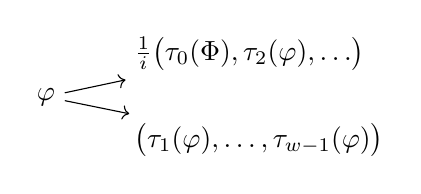
\begin{tikzpicture}
\node (phi) at (0,0) {$\varphi$};
\node[anchor=west] (even) at (1,0.55) {$\frac1i\bigl(\tau_0(\Phi),\tau_2(\varphi),\ldots\bigr)$};
\node[anchor=west] (odd) at (1,-0.55) {$\bigl(\tau_1(\varphi),\ldots,\tau_{w-1}(\varphi)\bigr)$};
\draw[->] (phi) -- (even);
\draw[->] (phi) -- (odd);
\end{tikzpicture}
\end{adjustbox}
\end{center}
В пр-вах периодов выд. подпр-ва, зад. ур-ями.
\begin{equation*}
S_{w+2}\begin{array}{cc}\nearrow&S^+\\\searrow&S^-\end{array}
\left.\vphantom{\begin{array}{c}S^+\\S^-\end{array}}\right\}
\underset{\mathrm{def}}{=}\text{пр-ва решений ур-й Sh.-Eich.}
\end{equation*}
\underline{Теорема.}
\begin{equation*}
\begin{aligned}
\text{а)}\quad&S_{w+2}\overset{\sim}{\longrightarrow}S^-\\
\text{б)}\quad&S_{w+2}\hookrightarrow S^+\qquad\text{влож.}\quad\operatorname{codim}1.
\end{aligned}
\end{equation*}
\underline{Теорема.}
\begin{equation*}
\begin{array}{ccc}
S_{w+2}&\overset{\sim}{\longrightarrow}&S^-\\
T_p&&\begin{adjustbox}{max width=\linewidth}
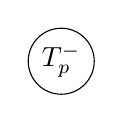
\begin{tikzpicture}[baseline=-0.5ex]\node[draw,circle,inner sep=2pt] {$T_p^-$};\end{tikzpicture}
\end{adjustbox}\\
&&\text{матрица из }\mathbb Z[\lambda_p]
\end{array}
\qquad\text{(оп. Гекке).}
\end{equation*}
Здесь
\begin{equation*}
(\Phi\mid T_p)(z)=p^{w+1}\varphi(pz)-p^{-1}\sum_{k=0}^{p-1}\varphi\left(\frac{z+k}{p}\right)
\end{equation*}
\Unclear{GELFAND-P000510}{hecke-minus}{Перед $p^{-1}\sum$ стоит минус.}
Соб. ф-и опер. Гекке $\Leftrightarrow$ [Зачёркнуто: \Incomplete{GELFAND-P000510}{hecke-cancellation}{Короткий текстовый фрагмент под густой правкой не восстановлен.}] разлаг. в Эйл. произвед.

$T_p^-$ — запись в терм. периодов (лин. форма однозн. опред.)

\underline{Приложение.}
\begin{equation*}
w=10,\quad S_{12}=R\cdot e^{2\pi iz}\prod_{n=1}^{\infty}(1-e^{2\pi inz})^{24}
=R\left(\sum_{n=1}^{\infty}\tau(n)e^{2\pi inz}\right)
\end{equation*}
(ф-я Рамануджана)

\underline{Тожд. Рамануджана}
\begin{equation*}
\tau(n)\equiv\sum_{d\mid n}d^{11}\pmod{691}
\end{equation*}
\SourcePage{GELFAND-P000511}{unlabelled}
% Original 2360 x 3400; inspected complete frame and strips (50,0,2310,920),
% (50,875,2310,1730), (50,1660,2310,2510), (50,2440,2310,3390).
% Pixel coordinates use (left, top, right, bottom), origin at upper left.
\underline{Меры.}
\begin{equation*}
P^+(x)=\frac{i}{\omega^+}\operatorname{Im}\int_x^{i\infty}\phi(z)\,dz,
\qquad
P^-(x)=\frac{1}{\omega^-}\operatorname{Re}\int_x^{i\infty}\Phi(z)\,dz
\end{equation*}
\begin{equation*}
\mu_\phi^\pm\bigl(a+(p^{m+1})\bigr)
\underset{\mathrm{def}}{=}
\rho^{-m}P^\pm\left(\frac{a}{p^{m+1}}\right)
-p^w\rho^{-(m+1)}P^\pm\left(\frac{a}{p^m}\right)
\end{equation*}
\Unclear{GELFAND-P000511}{measure-overwriting}{В последнем члене переписаны $P$ и показатель при $p$: чтение $P^\pm(a/p^m)$.}
меры с алг. знач. и можно
\Unclear{GELFAND-P000511}{measure-note}{пополнять / пополнить}.

\underline{Рост.} $P^\pm$ им. огранич. знаменатели. Они могут вылезти из-за $\rho$.
\begin{equation*}
\rho^2-\lambda_p\rho+p^{w+1}=0
\end{equation*}
\begin{equation*}
\begin{cases}
\rho_1\cdot\rho_2=p^{w+1},\\
\rho_1+\rho_2=\lambda_p.
\end{cases}
\end{equation*}
Тип. случай: \underline{$\lambda_p$ вз. пр. с $p$}
$\Rightarrow$ один корень даёт огр. меру, другой растущую!

Неизв. связь [зачёркнуто:
\Incomplete{GELFAND-P000511}{cancelled-middle}{Зачёркнутая запись между «связь» и $\lambda_p$ не прочитана.}]
$\lambda_p$ и $p$.

\underline{Интегралы}
(пр. Меллина от $p$-ад. хар.)
% «от» resolved by renewed original crop (1100,1145,1295,1250), 8x.
\begin{equation*}
\ldots\int_{Z_p^*}\chi\,d\mu_\Phi^\pm
\end{equation*}
Манин умеет лишь для хар. конечного пор. $\chi:Z_p^*\to K^*$,
$\chi^m=1$ и примитивный.

\underline{Теорема.}
\begin{equation*}
\ldots\int_{Z_p^*}\chi\,d\mu_\phi^\pm=\ldots L_\phi(1,\chi),
\end{equation*}
где
\begin{equation*}
L_\Phi(s,\chi)=\sum_{n=1}^{\infty}\chi(n)a_n n^{-s}
\end{equation*}
\begin{equation*}
\ldots \dot L_\phi(1,\chi)=\ldots\int_{R_+^*}\phi_\chi(z)\,dz,
\qquad\text{где }\Phi_\chi=\sum\chi(n)a_n e^{2\pi i n z}.
\end{equation*}
\Unclear{GELFAND-P000511}{l-dot}{Над $L$ в этой строке видна отдельная точка; её значение не установлено.}

\underline{О гипотезах Лихтенбаума: о связи $K$-групп, алг. полей с $\zeta$-ф-ми в цел. точках.}
\begin{equation*}
\sum_{n=1}^{\infty}\frac{1}{n^2}=\frac{\pi^2}{6},\qquad
\sum_{n=1}^{\infty}\frac{1}{n^3}=2\pi^2\lvert K_4 Z\rvert\cdot e_5(\alpha_5)
\end{equation*}
[Под второй суммой:] Впервые есть гипотеза

$\alpha_5$ — образующая $K_5 Z$. (своб. части)

$e_5$ — гомом. в вещ. числа (нек-рый)

Не док., что $\displaystyle\sum_1^\infty\frac{1}{n^3}$ трансценд.
Пост. Эйлера тоже не док.

[Внизу прямоугольная зачёркнутая запись:]
\Incomplete{GELFAND-P000511}{cancelled-bottom}{Текст внутри густо заштрихованного прямоугольника не прочитан.}

\SourcePage{GELFAND-P000512}{unlabelled}
% Original 2360 x 3400 inspected in full and in four overlapping strips.
% Strip bounds: (50,0,2310,920), (50,875,2310,1730),
% (50,1660,2310,2510), (50,2440,2310,3390).
[У правого верхнего края:]
\Unclear{GELFAND-P000512}{upper-right-edge}{Обрезанные штрихи; чтение отсутствует.}

\underline{\underline{24.9.73.}}\qquad\underline{\underline{Сем. Гельфанда.}}

\underline{Пинкус}; \underline{Дуглас, Кобурн,
\Unclear{GELFAND-P000512}{upper-names}{Вилнейр / Виннейр} и Зингер};
\underline{Хелтон и Роджер Хау. (Howe)}

(интересные работы по функц. анализу).

\underline{Теорема} (\underline{Helton, How}).
близко к раб. Крейна, Гохберга, Симоненко и т. д.

Пусть $B$ — билин. форма от 2-х многочленов
[вставлено над строкой, обведено и соединено стрелкой: от 2 перем.], причем
\begin{equation*}
B(P_1(Q),P_2(Q))=0,
\end{equation*}
если $P_1(z),P_2(z)$ — полин. от 1-го пер. $z$,
а $Q$ — полин. от любого числа перем. Тогда
\begin{equation*}
B(R,S)=L(\{R,S\}),\qquad \{R,S\}\text{ — скобка Пуассона}
\end{equation*}
\underline{$L$ — лин. форма.}

[Разделительный штрих, точка, штрих.]

Пусть $U,V$ — самосопр. и такие, что они коммутируют $\bmod$ ядерных.
Тогда
\begin{equation*}
\operatorname{Tr}\{[R(U,V),S(U,V)]\}=\iint\{R,S\}\,d\sigma
\end{equation*}
$R,S$ — многочлены; порядок в них $U$ и $V$ безразличен.

[Разделительный штрих, точка, штрих.]

\underline{Кн}\quad\underline{Douglas'а}\quad\underline{Banach algebras technique.}

$\Rightarrow$ в $p$-адич. случае вместо дифф. операторов нужны прав. подобранные
норм. кольца.

[Разделительный штрих, точка, штрих.]

\underline{Кириллов.}

\underline{L. Brown, R. Douglas, P. Fillmore.}

\underline{Расширения бан. алгебр (нетрадиц. типа).}

$\mathcal K$ — алг. комп. операторов в сеп. гильб. пр-ве.

\underline{Опр. 1.}
\begin{equation*}
0\to\mathcal K\to\mathcal A\to C(X)\to0,
\qquad X\text{ — компакт.}
\end{equation*}
Расш. обр. группу $\operatorname{Ext}(X)=\operatorname{Ext}_1(X)$.

\underline{Другое определение даёт ту же группу:}

\underline{Опр. 2.}
\begin{equation*}
C(X)\hookrightarrow\mathcal L/\mathcal K
\end{equation*}
[Под формулой проведена двойная скобка.]

1) рассм. все влож.

2) вложе., отлич. на унит. опер., отождествл.
(ун. экв. $UAU^{-1}$).

3) Вложе. вида $C(X)\to\mathcal L\to\mathcal L/\mathcal K$ счит. трив.

Классы эквив. тогда обр. группу.

\begin{center}
\begin{adjustbox}{max width=\linewidth}
\begin{tikzcd}
C(X) \arrow[r,shift left=0.6ex,"\tau_1"]
     \arrow[r,shift right=0.6ex,swap,"\tau_2"] & \mathcal L/\mathcal K
\end{tikzcd}
\end{adjustbox}
\end{center}
$\tau_1\oplus\tau_2$ уже в $H_1\oplus H_2\cong H$.

Функтор $\underline{\mathrm{Top}}\longrightarrow\underline{\mathrm{Ab}}$.

\underline{Осн. результат:} функтор $\operatorname{Ell}(X)$ сводится к
$\operatorname{Ext}(X)$ (отв. на вопрос Атьи).
\begin{equation*}
\operatorname{Ext}_{1-n}(X)=\operatorname{Ext}(S^nX)
\end{equation*}
[Под $S^nX$ с коротким указателем:] $n$-кр. надстройка.

\SourcePage{GELFAND-P000513}{14}
% Original 2360 x 3400 inspected in full and in overlapping strips:
% (50,0,2310,920), (50,875,2310,1730), (50,1660,2310,2510),
% (50,2440,2310,3390). Visible page label 14 at upper right.
\underline{Т. 1.} Точная послед.
\begin{equation*}
\operatorname{Ext}_1(A)\to\operatorname{Ext}_1(X)\to
\operatorname{Ext}_1(X/A)\to\operatorname{Ext}_0(A)\to\ldots
\end{equation*}
$A\subset X$

\underline{Т. 2.} Есть спаривание
\begin{equation*}
K^1\times\operatorname{Ext}_1\to\operatorname{Ext}_0
\end{equation*}
\begin{equation*}
K^1(X\times Y)\times\operatorname{Ext}_1(X)\to K^0(Y)
\end{equation*}
[Зачёркнуто: Функтор $\operatorname{Ext}_1$
\Unclear{GELFAND-P000513}{cancelled-upper-word}{вычислен}
для всех
\Incomplete{GELFAND-P000513}{cancelled-upper-end}{Конец зачёркнутой строки не прочитан.}]

[Подчёркнуто скобкой:]
\Unclear{GELFAND-P000513}{ext-operation}{$\operatorname{Ext}_1\oplus Z=K_0$ / $\operatorname{Ext}_1\otimes Z=K_0$}
для симплиц. комплексов.

\underline{Пример расширения.}
\begin{equation*}
0\to\mathcal K\to C^*(\text{„}ax+b\text{”})\to C(\infty)\to0
\end{equation*}
\begin{equation*}
\operatorname{Ext}(\infty)=Z+Z.
\end{equation*}
Какова эта пара чисел для конкр. опер.?

[Разделительный штрих, точка, штрих.]

[Слева зачёркнуто:]
\Unclear{GELFAND-P000513}{cancelled-torus}{$X=S^1$}
\begin{equation*}
X=\mathbb T=S^1
\end{equation*}
\begin{equation*}
C(\mathbb T)\to\mathcal L/\mathcal K
\end{equation*}
[Под $C(\mathbb T)$:] порожд. $z$ как алг. с инвол.

Пусть $T$ — образ $z$.
\begin{equation*}
TT^*=1\bmod\mathcal K
\end{equation*}
\underline{с точн. до унит. эквив. и $\bmod\ 1+\mathcal K$.}

\underline{Ответ:}\quad\underline{\underline{индекс}}\quad(классифик.).

[Разделительный штрих, точка, штрих.]

\underline{Теор.} $\{N+\mathcal K\}$ — замкн. по норме во всех опер.,
[под $N$ с коротким указателем: норм.]

а [зачёркнуто: $N_1N_2=N_2N_1$]
пары $\{N_1+K_1,\ N_2+K_2\}$ с усл. $N_1N_2=N_2N_1$
[вставлено слева и обведено: незамкнуто;
ниже зачёркнуто:
\Unclear{GELFAND-P000513}{cancelled-notclosed}{незамкнуто}]
в мн-ве всех пар такого вида.

\underline{След. раз:}\quad\underline{докл. Фукса;}\quad\underline{предст. по Мищенко.}

\underline{Фукс.}\qquad\underline{Quillen}\qquad\underline{Higher algebraic $K$-theory I}

(Proc. of symp. on $K$-theory)

\underline{Introduction.} $M$ — категория (абелева либо спец. аддитивная).
Определяются $K_i(M)$.

\underline{Построения.}

$QM$ — катег. частных $\Rightarrow$ классиф. пр-во $BQM$ $\Rightarrow$
\begin{equation*}
\Rightarrow\quad K_i(M)=\pi_{i+1}(BQM).
\end{equation*}
\underline{Essential part.}

Симпл. объект в категории $S$ — контравар. функтор $\mathrm{Ord}\to S$,
где $\mathrm{Ord}$ — кан. категория из неотриц. целых чисел.

% Diplomatic transcription of original frames; no catalogue-derived heading.
% All three 2360 x 3400 originals inspected at source resolution.
\SourcePage{GELFAND-P000514}{unlabelled}
% Coverage: original bbox (165,15,2115,605), crop scale 3.
\Unclear{GELFAND-P000514}{top-functor}{$\mathrm{Ord}^{\circ}\longrightarrow S$}

(Функтор всегда означает ковар. функтор)

$\mathrm{Ord}$ объекты — $0,1,2,3,\ldots$

Морф. \Incomplete{GELFAND-P000514}{upper-cancellation}{Зачёркнутая последовательность после «Морф.» не поддаётся прочтению.}
$p\to q$ наз. монотонно неубыв. отображение
\begin{equation*}
(0,1,\ldots,p)\longrightarrow(0,1,\ldots,q)
\end{equation*}
Все они предст. в виде композ. морф. 2-х сортов:

% Coverage: bbox (170,630,1700,1140), crop scale 3.
% The left omission rows are three horizontal strokes, not vertical dots.
% The small comma-like mark following the first 0 is retained.
% Two separate columns in the source. No arrows are supplied in rows
% where the right-hand source table has only aligned numerals.
\begin{equation*}
\begin{array}{c@{\qquad\qquad}c}
1).\quad\underline{p\longrightarrow p+1}&
2).\quad\underline{p+1\longrightarrow p}\\[4pt]
\begin{array}{ccc}
0,&\longrightarrow&0\\
-&-&-\\
i-1&\longrightarrow&i-1\\
i&\longrightarrow&i+1\\
-&-&-\\
p&\longrightarrow&p+1
\end{array}
&
\begin{array}{ccc}
0&&0\\
\vdots&&\vdots\\
i&\longrightarrow&i\\
i+1&\longrightarrow&i\\
\vdots&&\vdots\\
p+1&&p
\end{array}
\end{array}
\end{equation*}

% Coverage: bbox (160,1160,1870,1440), crop scale 3.
Для задания симпл. об. дост. указ. посл. объектов
$S_0,S_1,S_2,\ldots$
и морфизмов

% Coverage: bbox (295,1460,1400,1885), crop scale 3.
\begin{center}
\begin{adjustbox}{max width=\linewidth}
\begin{tikzcd}[column sep=large]
S_0 & S_1 \arrow[l,shift left=0.5ex] \arrow[l,shift right=0.5ex]
& S_2 \arrow[l,shift left=1ex] \arrow[l] \arrow[l,shift right=1ex]
& \cdots \arrow[l,shift left=1.5ex] \arrow[l,shift left=0.5ex]
\arrow[l,shift right=0.5ex] \arrow[l,shift right=1.5ex]
\end{tikzcd}
\end{adjustbox}
\end{center}
(отвечают вложениям типа 1))

и
\begin{center}
\begin{adjustbox}{max width=\linewidth}
\begin{tikzcd}[column sep=large]
S_0 \arrow[r] & S_1 \arrow[r,shift left=0.5ex] \arrow[r,shift right=0.5ex]
& S_2 \arrow[r,shift left=1ex] \arrow[r] \arrow[r,shift right=1ex]
& S_3 \arrow[r,shift left=1.5ex] \arrow[r,shift left=0.5ex]
\arrow[r,shift right=0.5ex] \arrow[r,shift right=1.5ex] & \cdots
\end{tikzcd}
\end{adjustbox}
\end{center}

% Coverage: bbox (190,1880,1800,2320), crop scale 3.
(отвеч. отобр. типа 2))

(Соотношения должны быть выполнены).

\hspace{3em}их легко выписать

$S$ — или кат. мн-в или кат. топ. пр-в.

% Semicolon verified at bbox (910,2240,975,2305), scale 8; heading colon
% below verified at bbox (210,2155,1900,2415), scale 3.
Но можно: группы; гладк. мн-зия и т.п.

% Coverage: bbox (115,2315,2330,2750), crop scale 3.
% The heading is double-underlined in the original.
\underline{\underline{Важный пример:}} сингу. комплекс топ. пр-ва.
$S$ — кат. множеств.

$X$ — топ. пр-во. \Unclear{GELFAND-P000514}{lower-notation}{Обозн.}
$S_q$ — все сингу. симплексы $X$

\Unclear{GELFAND-P000514}{singular-parenthesis}{(}непр. отобр. $\Delta^q\to X$, где
\begin{equation*}
\Delta^q=\{(x_1,\ldots,x_{q+1})\in R^{q+1},\quad x_i\ge0,\quad\sum x_i=1\}.
\end{equation*}
% The initial textual parenthesis has no matching closing parenthesis here.
\Unclear{GELFAND-P000514}{lower-face-symbol}{$\exists\delta_i:\Delta^{q-1}\longrightarrow\Delta^q$}
канонич. отобр. на $i$-ю грань (верш. упоряд.)

% Coverage: bbox (195,2760,2300,3340), crop scale 3.
\Unclear{GELFAND-P000514}{lower-singular-abbreviation}{Син.} симпл. — композиция
$\Delta^{q-1}\longrightarrow\Delta^q\longrightarrow X$

Получ. $q+1$ отображение
\begin{equation*}
S_q\quad
\begin{array}{c}\longrightarrow\\\cdots\\\longrightarrow\end{array}
\quad S_{q-1}\qquad\text{(грани).}
\end{equation*}
\begin{equation*}
\begin{gathered}
S_q\quad
\begin{array}{c}\longrightarrow\\\cdots\\\longrightarrow\end{array}
\quad S_{q+1}\\
(q+1\ \text{шт.})
\end{gathered}
\end{equation*}
из $\Delta^{q+1}\longrightarrow\Delta^q$ аффинные проекции
($i$-я склеив. $i$-ю верш. с $(i+1)$-й).

% A two-stroke separator and a dot end the written portion.
\begin{center}
\begin{adjustbox}{max width=\linewidth}
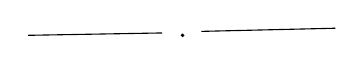
\begin{tikzpicture}
\draw (0,0)--(1.7,0.03);
\draw (2.2,0.05)--(3.9,0.09);
\fill (1.96,0) circle (0.025);
\end{tikzpicture}
\end{adjustbox}
\end{center}

\SourcePage{GELFAND-P000515}{15}
% Coverage: bbox (145,20,2320,530), crop scale 3.
\underline{Реализация.}

Пусть $S$ — кат. мн-в или топ. пр-в.

Симпл. об. в кат. мн-в или топ. пр-в относится топ. пр-во.

% "м-ва" is an authorial interlinear insertion, circled with a tail
% into the gap after "Элементы". The sentence is wavy-underlined.
\underline{Элементы} [вставлено над строкой, обведено: м-ва] \underline{$S_i$ наз. симплексами}

\underline{Образы стрелок слева направо наз. вырожд. симплексами.}

% Both following sentences are wavy-underlined in the source;
% cross-review bbox (180,420,2320,535), scale 3.
\underline{Прочие наз. невырожденными.}
\underline{\Unclear{GELFAND-P000515}{nondegenerate-faces}{Стр. справа налево перев. невыр. в невырожденные.}}

% Coverage: bbox (135,530,2310,1130), crop scale 3.
Рассм. $\Delta^q\times S_q^0$

\hspace{3em}невыр. симп. из $S_q$.
\qquad ($S_q^0$ — дискр. топ. пр-во).

В $\coprod_q\Delta^q\times S_q^0$ (несвязн. объединение) отождествление.

\begin{equation*}
\Delta^{q-1}\times s,\qquad s\in S_{q-1}^0
\end{equation*}
отожд. с частью $\Delta^q\times s'$,
\Unclear{GELFAND-P000515}{gluing-membership}{$s\in S_q^0$},

когда $s$ — образ $s'$ при отобр. ($i$-м)
\begin{equation*}
S_{q-1}\overset{i}{\longleftarrow}S_q\qquad\text{($i$-я грань)}
\end{equation*}

% Coverage: bbox (140,1115,2340,1740), crop scale 3.
\underline{Получ. топ. пр-во.} \underline{Это клеточное пр-во} (не склеив. внутренности).

Но: точки границы могут склеиться (так что не симплиц. пр-во)!

То же прим., если $S$ — топ. пр-ва.
\Unclear{GELFAND-P000515}{topological-wording}{Уже не возникает топ. структ.},

т.к. в $\Delta^q\times S_q^0$ топ. прямого произв.

\underline{\underline{Упр.:}} для хорошего топ. пр-ва реализация сингу.
\Incomplete{GELFAND-P000515}{middle-cancellation}{Зачёркнутое слово после «сингу.» не поддаётся прочтению.}
комплекса

гомотоп. эквив. $X$.

Для \Unclear{GELFAND-P000515}{polyhedron-abbreviation}{восстан.} полиэдра надо принять за $S_i$ афф. отобр. симплексов туда

% Figure inspected in original bbox (300,1690,472,1845), scale 6.
% Five-sided boundary and five spokes; the source has small pen gaps
% at the lower-left boundary and at the corresponding spoke endpoint.
\begin{center}
\begin{adjustbox}{max width=\linewidth}
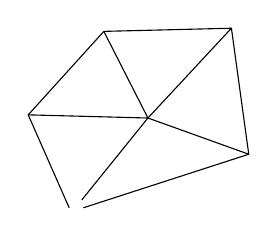
\begin{tikzpicture}[x=0.02cm,y=-0.02cm]
\draw (64,25)--(145,23)--(156,103)--(51,137);
\draw (42,137)--(16,78)--(64,25);
\draw (92,80)--(64,25);
\draw (92,80)--(145,23);
\draw (92,80)--(156,103);
\draw (92,80)--(50,132);
\draw (92,80)--(16,78);
\end{tikzpicture}
\end{adjustbox}
\end{center}

\underline{Реализация коммут. с умножением.}

% Coverage: product sketches bbox (215,1925,1600,2615), scale 3.
% Literal arrangement: the lower right arrow has no written source;
% the diagonal dividing line and detached southwest arrow remain detached.
\begin{center}
\begin{adjustbox}{max width=\linewidth}
\begin{tikzpicture}[x=0.008cm,y=-0.008cm]
\node at (75,40) {$S'_0$};
\node at (265,55) {$\cdots$};
\draw[->] (183,30)--(128,30);
\draw[->] (183,60)--(128,60);
\node at (112,168) {$S_0\times S'_0$};
\node at (405,168) {$S_1\times S'_1$};
\draw[->] (285,146)--(217,146);
\draw[->] (285,187)--(217,187);
\draw (665,2)--(767,217);
\node at (810,32) {$\mathcal S\times\mathcal S'$};
\node at (1100,32) {$\mathcal S$};
\node at (1100,111) {$\mathcal S'$};
\draw[->] (949,33)--(1045,33);
\draw[->] (949,108)--(1030,108);
\draw[->] (795,245)--(754,288);
\end{tikzpicture}
\end{adjustbox}
\end{center}

отсюда
\begin{center}
\begin{adjustbox}{max width=\linewidth}
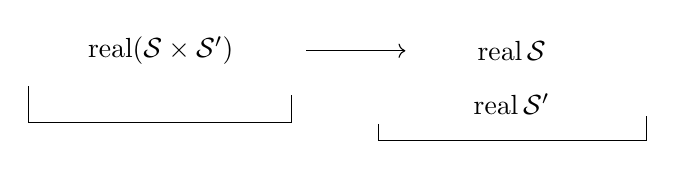
\begin{tikzpicture}[x=0.009cm,y=-0.009cm]
\node at (205,40) {$\operatorname{real}(\mathcal S\times\mathcal S')$};
\node at (700,40) {$\operatorname{real}\mathcal S$};
\node at (700,115) {$\operatorname{real}\mathcal S'$};
\draw[->] (410,40)--(550,40);
\draw (18,90)--(18,141)--(390,141)--(390,103);
\draw (512,143)--(512,166)--(890,166)--(890,132);
\end{tikzpicture}
\end{adjustbox}
\end{center}

и они составляют
\begin{equation*}
\underline{\underline{\operatorname{real}(\mathcal S\times\mathcal S')\longrightarrow
\operatorname{real}\mathcal S\times\operatorname{real}\mathcal S'.}}
\end{equation*}

% Coverage: bbox (15,2570,1485,2690), crop scale 3.
% "Оказ., что оно" is wavy-underlined; "Утв." has two straight strokes.
\underline{\underline{Утв.}} \underline{Оказ., что оно} — \underline{\underline{гомеоморфизм.}}

% Coverage: bbox (75,2680,1450,3215), crop scale 3.
\underline{Пример.}
\begin{center}
\begin{adjustbox}{max width=\linewidth}
\begin{tikzpicture}
\draw (0,0)--(1.2,0);
\draw (0,-0.09)--(0,0.09);
\draw (1.2,-0.09)--(1.2,0.09);
\end{tikzpicture}
\end{adjustbox}
\end{center}
Упор. отрезок.

$S^0$ — 2 элемента

$S^1$ — 3 элем. (с учетом вырожд.)

\Unclear{GELFAND-P000515}{lower-overwritten-exponent}{$S^p$}
$=(p+2)$ элем. $i$-й:
\begin{equation*}
[0,i-1]\longrightarrow0;\qquad[i,p]\longrightarrow1
\end{equation*}
$S_p\times S_p$

(в следующий раз.)

\SourcePage{GELFAND-P000516}{unlabelled}
% Coverage: bbox (45,15,2310,355), crop scale 3.
\underline{§2. Классиф. пр-во в категории.}

$C$ — категория (малая). С ней связ. её нерв $NC$ (симпл. объект кат. множеств).

\begin{equation*}
NC_q=\{\text{\ReaderApparatusRef{1}{1}}\quad
X_0\longrightarrow\cdots\longrightarrow X_q\}
\qquad\text{мн-во таких диаграмм}
\end{equation*}

% Coverage: bbox (210,365,1510,1050), crop scale 3.
\underline{$NC_q\longrightarrow NC_{q-1}$}

\underline{0-е}
\begin{adjustbox}{max width=\linewidth}
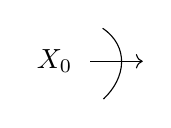
\begin{tikzpicture}[baseline=-0.5ex]
\node at (0,0) {$X_0$};
\draw[->] (0.45,0)--(1.12,0);
\draw (0.61,0.42) .. controls (0.95,0.19) and (0.91,-0.21) .. (0.62,-0.48);
\end{tikzpicture}
\end{adjustbox}
\qquad (отбросим).

\underline{$q$-е} — отбрас. $X_q$

\underline{\underline{$i$-е}} — композ. $i$ и $i+1$-й стрелок
\begin{center}
\begin{adjustbox}{max width=\linewidth}
\begin{tikzcd}[column sep=large]
\cdots \arrow[r] \arrow[rr,bend right=28] & X_i \arrow[r] & \cdots
\end{tikzcd}
\end{adjustbox}
\end{center}

\underline{$NC_q\longrightarrow NC_{q+1}$}

один из $X$ раздваивается и вставл. тожд. морфизм.

% Coverage: bbox (240,1055,2195,1390), crop scale 3.
\underline{\Unclear{GELFAND-P000516}{definition-cancellation}{[зачёркнуто: Нерв.]}}
$\operatorname{Real}NC=BC$ — классиф. пр-во категории.

\underline{Пример:} классиф. пр-во группы $G$ получ. из
\Unclear{GELFAND-P000516}{group-category-abbreviation}{след. катег.}:
\Incomplete{GELFAND-P000516}{group-cancellation}{Зачёркнутая последовательность после двоеточия не поддаётся прочтению.}

% "Элементы G." is wavy-underlined; cross-review bbox
% (1040,1280,1630,1410), scale 3.
1 объект, и морфизмы — \underline{Элементы $G$.}

\begin{equation*}
NC_q=\underbrace{G\times\cdots\times G}_{q}
\end{equation*}

% Separator checked at original bbox (720,1635,1115,1705), scale 6.
\begin{center}
\begin{adjustbox}{max width=\linewidth}
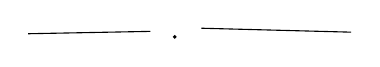
\begin{tikzpicture}
\draw (0,0)--(1.55,0.03);
\draw (2.2,0.07)--(4.1,0.02);
\fill (1.86,-0.04) circle (0.025);
\end{tikzpicture}
\end{adjustbox}
\end{center}

% Coverage: bbox (240,1675,2100,2070), crop scale 3.
$G=Z_2$. Симплексы:

\underline{Невыр. симп.} — не содержат 1.

По 1 невыр. симп. каждой размерности.

\SourceFigure{GELFAND-P000516}{exercise-margin-mark}{Слева от «Упр.» обведены кружком три длинных почти вертикальных штриха; у верхней левой части кружка есть тёмный пересекающийся знак.}
Упр. 2-мерная часть.
\Unclear{GELFAND-P000516}{exercise-word}{Дважды}.
Получается $RP_{\infty}$.

% Two-stroke separator with dot, immediately below the exercise.
\begin{center}
\begin{adjustbox}{max width=\linewidth}
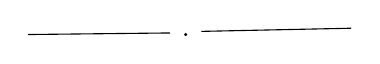
\begin{tikzpicture}
\draw (0,0)--(1.8,0.02);
\draw (2.2,0.04)--(4.1,0.08);
\fill (2,0) circle (0.022);
\end{tikzpicture}
\end{adjustbox}
\end{center}

% Coverage: bbox (160,2075,2330,2490), crop scale 3.
Пусть $M$ — категория, к-рая либо абелева, либо полная подкат.
абелевой кат., замкн. отн. взятия расширений. Пусть
классы изом. объектов сост. множество. Тогда она эквивалентна
малой категории. \underline{Категория $QM$.} \underline{$\operatorname{Ob}(QM)=\operatorname{Ob}(M)$}.

% Coverage: bbox (215,2470,2300,2920), crop scale 3.
% QM annotation leaders rechecked at (1225,2460,2215,2770), scale 4:
% the left leader points upward/right; the long right leader curves upward/left.
\begin{equation*}
\operatorname{Hom}_{QM}(X',X'')\ \Rightarrow\ \text{диаграммы}
\end{equation*}
\begin{center}
\begin{adjustbox}{max width=\linewidth}
\begin{tikzpicture}
\node at (0,0) {$X'$};
\node at (3,0) {$X$};
\node at (5.5,0) {$X''$};
\draw[->] (2.65,0)--(0.35,0);
\draw[->] (3.35,0)--(5.15,0);
\draw[->] (0.95,-1.4)--(1.65,-0.42);
\draw[->] (5.35,-1.92) .. controls (4.52,-1.55) and (3.98,-1.04) .. (3.9,-0.43);
\node[align=left,anchor=north west] at (-0.9,-1.8) {эпиморфизм\\с ядром};
\node[align=left,anchor=north west] at (5.65,-1.92) {мономорфизм\\с коядром};
\end{tikzpicture}
\end{adjustbox}
\end{center}

Это категория.

\underline{Определение.}

% Bottom formula and its open lower bracket are directly visible;
% original inspected through y=3400, including the blank bottom margin.
\begin{center}
\begin{adjustbox}{max width=\linewidth}
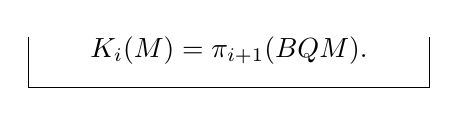
\begin{tikzpicture}
\node at (3,0) {$K_i(M)=\pi_{i+1}(BQM).$};
\draw (0.45,0.18)--(0.45,-0.47)--(5.55,-0.47)--(5.55,0.18);
\end{tikzpicture}
\end{adjustbox}
\end{center}


\ReaderNotesStart{GELFAND-P000516}
\ReaderNote{1}{\Unclear{GELFAND-P000516}{nerve-blot}{[неразборчивый знак]}}
\ReaderNotesEnd
\SourcePage{GELFAND-P000517}{unlabelled}
% Coverage review: original 2360x3400 at source resolution (1x); all visible content inspected.
% Enlarged coverage, original pixel bboxes: (140,15,1485,230) 3x; (0,240,1200,700) 3x;
% (1190,240,2340,700) 3x; (135,720,1220,1115) 3x; (1210,720,2300,1115) 3x;
% (330,1110,2280,1745) 3x; (100,1735,1270,2530) 3x; (1240,1735,2240,2530) 3x;
% (100,2520,1270,3370) 3x; (1240,2520,2270,3370) 3x. Outer margins reviewed in original.
\underline{Продолжение докл. Фукса} (по Марченко)

\underline{Пример реализации.}
% The original example heading has a wavy underline.

$S_q$ состоит из $q+2$ элементов. Интерпр. их как м-во афф. отобр.
$\Delta^q$ в отрезок $\Delta^1$, согласованных с упорядочением вершин $\Delta^q$ и $\Delta^1$.

Морфизмы $S_{q-1}\leftarrow S_q\to S_{q+1}$ опр. как для сингулярных симплексов
пр-ва $I=\Delta^1$ \fbox{(сужение на аффинные)}, т. е. композицией с вложением и ограничениями
% Boxed interlinear insertion, with a pointer after I=Delta^1: (390,540,935,626), inspected at 5x.
% Following words inspected at 4x in (470,620,2100,697); source singular «вложением» retained.

Невырожд. симплексы — 2 0-мерных $*\to I$ и 1 одномерный.

$S_q\times S_q$ когда элемент $S_q\times S_q$ невыр. ?

Элм. — пара $(\varphi,\psi)$, он невыр., когда нет 2-х вершин в $\Delta^q$, отображаю-\\
щихся $\varphi$ и $\psi$ \Unclear{GELFAND-P000517}{cancelled-sign}{Зачёркнутый знак неразборчив.}
в одну \Incomplete{GELFAND-P000517}{cancelled-word}{Зачёркнутое слово неразборчиво.} вершину

\begin{equation*}
S_0\times S_0\quad\text{— 4 элм.}\quad *\to(0,0),(0,1),(1,0),(1,1)
\end{equation*}
\begin{equation*}
S_1\times S_1\qquad
\binom{1}{0}\to
\begin{matrix}\varphi&\psi\\0&0\\0&1\end{matrix}
\qquad
\left(\begin{matrix}0&1\\0&1\end{matrix}\ \text{вырожд.}\right)
\left(\begin{matrix}0&0\\1&1\end{matrix}\right)
\left(\begin{matrix}0&0\\1&0\end{matrix}\right)
\left(\begin{matrix}0&1\\1&1\end{matrix}\right)
\left(\begin{matrix}1&0\\1&1\end{matrix}\right)
\end{equation*}
\Unclear{GELFAND-P000517}{array-cancellation}{После второго столбца матрицы перед «вырожд.» зачёркнут знак, похожий на закрывающую скобку.}
\begin{equation*}
S_2\times S_2\qquad \Delta\to
\begin{matrix}0&0&0&0\\1&0&0&1\\1&1&1&1\end{matrix}
\end{equation*}

Реализация $S\times S$
\SourceFigure{GELFAND-P000517}{realization-square}{Четырёхугольник с диагональю из нижнего левого в верхний правый угол. На левой и правой сторонах стрелки направлены вверх, на верхней стороне вправо, на диагонали к верхнему правому углу. У правого конца нижней стороны виден загнутый штрих; направление нижней стороны не установлено. Подписей вершин нет.}

\underline{Классиф.} \underline{пр-во} \underline{категории.}

$C$ — малая кат., $NC$ — нерв категории

$(NC)_q\ (=S_q)$ — все диагр. $C$ вида $X_0\to\ldots\to X_q$

отобр. — взятие композ., \Unclear{GELFAND-P000517}{endpoint-abbreviation}{отбрс.} концов и вставление $\mathrm{id}$ \Unclear{GELFAND-P000517}{identity-index}{$X_j$}.

\begin{equation*}
BC=\mathrm{Real}\,NC.
\end{equation*}

Вершины $BC$ — объекты $C$, 1-мерные симплексы — нетождественные
морфизмы. $\Delta$ натягиваются на коммутативные симплексы
\begin{adjustbox}{max width=\linewidth}
\begin{tikzcd}[column sep=small,row sep=small]
 & {} \arrow[dr] & \\
{} \arrow[ur] \arrow[rr] & & {}
\end{tikzcd}
\end{adjustbox}
% Unlabelled commutative triangle at original bbox (2030,2370,2165,2458), inspected at 3x.
и т. д.

Барицентрич. \Unclear{GELFAND-P000517}{subdivision-abbreviation}{подразб.} полиэдра высокой степ. — нерв нек-рой категории.

\underline{Св-ва.}
\begin{equation*}
B(C\times C')\cong BC\times BC'
\end{equation*}
\begin{equation*}
f:C\rightsquigarrow C'\quad\Rightarrow\quad Bf:BC\to BC'
\end{equation*}
Если есть ещё $g:C\to C'$ и естеств. отобр. $f$ в $g$, то $Bg:BC\to BC'$
связывается с $Bf$ канонической гомотопией.

Пусть $\{0,1\}$ — кат. из 2-х объектов с одним морфизмом $0\to1$

Морфизм функторов $f$ и $g$ — функтор из $C\times\{0,1\}$ в $C'$.

\SourcePage{GELFAND-P000518}{21}
% Coverage review: original 2360x3400 at source resolution (1x); all visible content inspected.
% Enlarged coverage, original pixel bboxes: (110,50,1200,865) 3x; (1180,40,2330,865) 3x;
% (110,875,1230,1700) 3x; (1205,875,2340,1700) 3x; (90,1680,1250,2510) 3x;
% (1230,1680,2355,2510) 3x; (110,2490,1260,3355) 3x; (1230,2490,2355,3355) 3x.
% Narrow checks: (406,746,678,850) 6x, superscript circle; (1910,2790,2360,2895) 5x, right-edge BC';
% (180,3010,500,3120) 6x, quantified morphism v. Outer margins reviewed in original.
$F:C\times\{0,1\}\to C'$. На концах $f,g$; морф. $0,1$ — естеств. отобр.

Он определяет отобр. — гомотопию, связывающую $f$ с $g$
\begin{equation*}
BC\times I=B(C\times I)\to BC'.
\end{equation*}

Если $C$ имеет финальный или начальный объект, то $BC$ стягиваемо —\\
— оно конус.

Если $f:C\rightsquigarrow C'$ имеет левый или правый сопряженный, то
$Bf$ — гомотопическая эквивалентность.
\begin{equation*}
BC^{\circ}=BC,\qquad B(C\times C')=BC\times BC'.
\end{equation*}

\underline{Аналог гомотопич. послед. расслоения.}

Пусть $f:X\to Y$ — рассл. Серра. Тогда
\begin{equation*}
\ldots\to\pi_q(X,x)\to\pi_q(Y,f(x))\to\pi_{q-1}(f^{-1}(f(x),x)\to\pi_{q-1}(X,x)\to\ldots
\end{equation*}
\Unclear{GELFAND-P000518}{fibre-parentheses}{В члене $\pi_{q-1}(f^{-1}(f(x),x)$ скобки непарные в источнике; написание оставлено без исправления.}

Если $f$ не уд. акс. о накр. гомот., то после замены на эквив. будет
ей удовл. и получим послед. Вот конструкция:

Пусть $\widetilde X=\{(x,s),\ x\in X;\ s:I\to Y,\ s(0)=f(x)\}$.

$\widetilde X\underset{\sim}{\supset}X$. Отобр. $\widetilde f:\widetilde X\to Y$ строится так:

$\widetilde f(x,s)=s(1),\qquad\widetilde f|_X=f$ но уже есть акс. накр. гом.

Из-за $\widetilde X$ \Unclear{GELFAND-P000518}{homotopy-relation}{$\simeq$} $X$ имеем точную послед.
\begin{equation*}
\ldots\to\pi_q(X)\to\pi_q(Y)\to\pi_{q-1}(\text{гомот. слой})\to\pi_{q-1}(X)\to\ldots
\end{equation*}

Пусть теперь \underline{$g:C\rightsquigarrow C'$}, тогда есть

$Bg:BC\rightsquigarrow BC'$. Хочется постр. „гомотопич. слой“ $Bg$.

Это не сделано, есть суррогат.

Констр. зависит ещё от нек. объекта $Y\in\mathrm{Ob}\,C'$.

Опр. категорию $Y\backslash g$. $\mathrm{Ob}(Y\backslash g)$ — пары $(X,u)$, где

$X\in\mathrm{Ob}\,C,\quad u\in\mathrm{Mor}_{C'}(Y,g(x))$.

Морфизм $(x,u)$ в $(x',u')$ — морфизм $\varphi:X\to X'$, соглас. с $u$
и $u'$. Есть естеств. отображение $B(Y\backslash g)\to\text{гомот. слой }Bg:BC\to BC'$
\Unclear{GELFAND-P000518}{object-case}{В записи $g(x)$ и в парах $(x,u)$, $(x',u')$ виден строчный $x$, при прописном $X$ в предшествующих записях; регистр сохранён.}

\underline{Теорема.} Пусть функтор $g$ таков, что

$\forall v\in\mathrm{Mor}_{C'}(Y,Y')$ возникающее отображение $Y'\backslash g\overset{v\backslash g}{\longrightarrow}Y\backslash g$

и $B(v\backslash g):B(Y'\backslash g)\to B(Y\backslash g)$ явл. гомот. эквивал. (что, вообще
говоря, неверно). Тогда $B(Y\backslash g)$ — гомот. слой $BC\overset{Bg}{\rightsquigarrow}BC'$.

\SourcePage{GELFAND-P000519}{unlabelled}
% Original frame 2360 x 3400 pixels. Coverage: (75,10)-(2235,765), top continuation and chains; inspected original and 3x crops.
Постр. отобр. $B(Y\backslash g)$ — гомот. слой $Bg$.

Если есть \Unclear{GELFAND-P000519}{simplex-index}{$(X_0,u_0)\leftarrow\cdots\leftarrow(X_\tau,u_\tau)$}
(симплекс $B(Y\backslash g)$)
то есть и \Unclear{GELFAND-P000519}{simplex-index}{$X_0\leftarrow\cdots\leftarrow X_\tau$}
и нужно знать лишь \Unclear{GELFAND-P000519}{simplex-index}{$Y\to g(X_\tau)$}
\Unclear{GELFAND-P000519}{unclosed-parenthesis}{(по нему восстанавливаются все $u_j$}

\Unclear{GELFAND-P000519}{simplex-index}{$X_0\leftarrow\cdots\leftarrow X_\tau$} — симплекс $BC$ размерности
\Unclear{GELFAND-P000519}{simplex-index}{$\tau$}.
Вместе с \Unclear{GELFAND-P000519}{simplex-index}{$u_\tau$} он опред. симплекс
\Unclear{GELFAND-P000519}{simplex-index}{$g(X_0)\leftarrow\cdots\leftarrow g(X_\tau)\overset{u}{\leftarrow}Y$}
в $BC'$.

% Coverage: (95,755)-(2330,1555), comparison paragraph, geometric sketch and right-side annotation; inspected at 3x, indices at 6x, small quantifier at 8x.
Таким обр., по симплексу в $B(Y\backslash g)$ мы определили 2
симплекса — в $BC$ и в $BC'$ размерностей
\Unclear{GELFAND-P000519}{simplex-index}{$\tau$ и $\tau+1$} соотв.
Симпл. из $B(Y\backslash g)$ отобр. так: точка пр-ва $BC$ соотв.
этой точке (в барицентр. координ.) и прямой путь в симплексе
$BC'$, соединяющий $Bg$ от этой точки в $Y$:

\SourceFigure{GELFAND-P000519}{simplex-sketch}{Слева над контуром треугольника написано $B(Y\backslash g)$; от него идёт стрелка вправо к другому треугольнику с подписью $BC$. От правого треугольника вниз идёт прерывистая линия возле $Bg$ к четырёхугольнику с диагональю из нижнего левого в верхний правый угол. У левой стороны четырёхугольника повторено $Bg$ поверх густых штрихов; эта часть рисунка не вполне различима.}

Это гомот. экв.
\Unclear{GELFAND-P000519}{sketch-quantifier}{$\forall v$}
iff вып. условия теоремы.

% Coverage: (105,1550)-(2300,2545), Fuchs remark and Mishchenko heading/definition; inspected at 3x, parenthetic bibliographic word at 8x.
\underline{Замеч. Фукса}: вероятно $Y\backslash g$ надо опр. как обр. пред.
по спектру всех \underline{$Y\backslash g$} с \underline{различными} $Y$.

\underline{\underline{Мищенко.}} (\underline{Представления по Мищенко})
% The parenthetic heading has a wavy underline in the source.

$\Lambda$ — кольцо с инволюцией, $H$ — гильбертово пр-во и 2 предст.
$T_1$ и $T_2$ кольца $\Lambda$ в алгебру огр. опер. в $H$, $F$ — фредгольмов
оператор в $H$ и пусть
\begin{equation*}
\forall\lambda\in\Lambda\qquad FT_1(\lambda)-T_2(\lambda)F\in\operatorname{Comp}(H)
\end{equation*}
Эта система $\{T_1,T_2,F\}$ наз. фредгольмовым предст. $\Lambda$.

Атья рассматривал $\Lambda=C(M)$, $M$ — многообразие
(лит-тура в \Unclear{GELFAND-P000519}{atiyah-parenthesis}{Токио}).

\underline{Констр. с этими пред}ставлениями

% Coverage: (50,2530)-(2265,3390), numbered constructions and continuation at lower edge; inspected at 3x, cancellation at 8x.
1) Атья (1970) $\Lambda=C(M)$\qquad
$\forall$ предст. сопост. $\operatorname{index}T\in K_0(M)$

2) $\Lambda=\mathbb Z[\pi]\quad\Rightarrow\quad\forall$ предст. строится
$\xi_T\in K^0(B_\pi)$.

3) $\Lambda$ — любое,\qquad
$A=(a_{ij})$ — квадр. форма на $\Lambda^n$\quad $(a_{ij}\in\Lambda)$
\begin{equation*}
A^*=A,\quad\exists A^{-1}\quad\Rightarrow\quad
\text{Строится }\operatorname{sign}_T A\in\mathbb Z.
\end{equation*}

\Unclear{GELFAND-P000519}{cancelled-number}{[зачёркнутый номер: неразборчиво]}
1) $\Lambda=C(M)$, $T$ — фредг. предст. $\Lambda$ в $H$,\quad $T=(T_1,T_2,F)$.

$H_i$ — модули над $\Lambda$.\qquad $\operatorname{ind}F$ — число.
Пусть $\eta$ — расслоение,
$\Gamma(\eta)$ — проект. модуль над $C(M)$. Рассмотрим
% No further legible source text at the lower border; continuation follows on P000520.

\SourcePage{GELFAND-P000520}{22}
% Original frame 2360 x 3400 pixels. Coverage: (160,25)-(2285,1040), page label, tensor arrow and index discussion; original and 3x crops, overwritten sign 6x, cancelled text 10x.
\begin{equation*}
H_1\otimes_{C(M)}\Gamma(\eta)
\overset{F\otimes 1_\eta}{\longrightarrow}
H_2\otimes_{C(M)}\Gamma(\eta)
\end{equation*}
\begin{equation*}
\operatorname{ind}(F\otimes1_\eta):K^0(M)\to\mathbb Z,
\quad\text{т.е. элемент }K_0(M)
\end{equation*}
Это грубовато из-за $\exists$ элем. конечного порядка в $K^0(M)$.

Точнее: $T$ опред. $\operatorname{index}_T:K^0(M\times Y)\to K^0(Y)$;\quad $\forall Y$.
Это уже элемент из $K_0(M)$.

Если $\sigma(A)\in K^0(T^*M)$,\quad $A:H\to H$;\quad т.к. $[f,A]$
\Unclear{GELFAND-P000520}{commutator-connector}{—}
комп., то есть
[Зачёркнуто: \Incomplete{GELFAND-P000520}{cancelled-before-index}{Короткая зачёркнутая группа знаков не прочитана.}]
$\operatorname{index}(A)\in K_0(M)$.
Так. эти элем. двойств. друг другу по Пуанкаре
$K^0(T^*M)\underset{\mathcal D}{\sim}K_0(M)$.
Тогда $\operatorname{index}A=\mathcal D(\sigma(A))$

(NB можно стр. \underline{прямой} образ $A$)

% Coverage: (120,1020)-(2300,2070), second construction, Fredholm operator space, covering action; inspected at 3x and interlinear ell-squared at 8x.
2) $\pi$ — произв. дискр. группа, $\Lambda=\mathbb Z[\pi]$ — её групп. кольцо, $B_\pi$ —
— классиф. пр-во. $T$ — фредг. предст. $T=(T_1,F,T_2)$. Надо постр.
$\xi_T\in K(B_\pi)$.

$K(B_\pi)$ понимаем как $[B_\pi,BU]$, но $BU\simeq\mathcal F$ (фредг. опер.)
% Source insertion below the parenthesis at (1910,1430)-(2180,1515):
[Вставлено под «фредг. опер.»: в $\ell^2$]
\begin{equation*}
B_\pi\ni x\to\Phi_x\in\mathcal F.
\end{equation*}
Пусть. $\Phi_x:H_1\to H_2$ там, где действовали $F$ из $T$,
$\widetilde B_\pi$ — универ. накр. $B_\pi$, где действует $\pi$.
Возьмём $\widetilde B_\pi\times H_i$ с действием $\pi$ на $\widetilde B_\pi$
стандартно, а на $H_i$ через $T_i$.
Пусть $\widetilde B_\pi$ — клет. комплекс (даже симплициальный).

% Coverage: (150,2070)-(2310,2925), construction on skeleta and equivariance; inspected at 3x, degree glyphs and membership at 8x/10x.
Постр. $\Phi_x:\widetilde B_\pi\times H_1\to\widetilde B_\pi\times H_2$.
Пусть $[\widetilde B_\pi]^k$ — $k$-мерн. остов $\widetilde B_\pi$.
Выб. по $\sigma_i^0$
\Unclear{GELFAND-P000520}{vertex-membership}{$\in$}
$[\widetilde B_\pi]^0$ в любой
орбите действия $\pi$ и положим $\Phi_{\sigma_i^0}\overset{\mathrm{def}}{=}F$.
Имеем:

а) эквивариантность

б) $\forall x,y\in[\widetilde B_\pi]^0\quad\Rightarrow\quad
\varphi_x-\varphi_y\in\operatorname{Comp}$
% The two operator letters in this displayed condition are the smaller looped phi forms visible in the source.

Прод. это на $[\widetilde B_\pi]^1$; в силу симплиц. действия $\pi$ можно
выбр. по симплексу в $\forall$ орбите и прод. на симплекс как
$p\Phi_1+q\Phi_2$, $p+q=1$ с вып. эквивариантности.
По инд. получим всё сем-во $\Phi_x$. Из эквивар. имеем

% Coverage: (90,2920)-(2350,3395), triangular bundle diagram and final two lines; inspected at 3x, surname and last operator at 8x.
\begin{adjustbox}{max width=\linewidth}
\begin{tikzcd}
(\widetilde B_\pi\times H_1)/\pi
\arrow[rr] \arrow[dr,"H_1"']
&&(\widetilde B_\pi\times H_2)/\pi \arrow[dl,"H_2"]\\
&\widetilde B_\pi/\pi=B_\pi&
\end{tikzcd}
\end{adjustbox}

Но из \Unclear{GELFAND-P000520}{kuiper-name}{Кёйпера}
$(\widetilde B_\pi\times H_i)/\pi\simeq B_\pi\times H_i$.
После отождеств. имеем $B_\pi\times H_1\to B_\pi\times H_2$,
задающее $\Phi_x:H_1\to H_2$.
\SourcePage{GELFAND-P000521}{unlabelled}
\underline{\underline{15/$\overline{\underline{X}}$-73}}\qquad \underline{Сем. Гельфанда.}

\underline{\underline{Рудаков.}}\qquad
\underline{О представлениях бесконечномерных алгебр Ли.}

Рассм. $W_n$ — алг. Ли форм. вект. полей
(дифф. кольца $k[[x_1,\ldots,x_n]]$).
[К слову «дифф.» снизу вписано и обведено: непр.]
\begin{equation*}
\left(\sum_{i=1}^{n}a_i(x_1,\ldots,x_n)\frac{\partial}{\partial x_i}\right)
\end{equation*}
\begin{equation*}
W_n=\mathcal L\supset
\Unclear{GELFAND-P000521}{upper-chain-cancel}{\text{[зачёркнутое обозначение: }M\text{?]}}
\;M\supset M'.
\end{equation*}
[Под $M$: подалг.]
\Incomplete{GELFAND-P000521}{upper-subalgebra-cancel}{Под словом «подалг.» две строки зачёркнуты плотными штрихами; исходные слова не читаются.}
[Под $M'$:] идеал конечн. коразм. в $M$.

Пусть дано предст. $M/M'\longrightarrow\text{предст. }M
\underset{\text{индуц.}}{\longrightarrow}\text{представл. }\mathcal L$.

\underline{Теор.:} все неприв. предст. $W_n$ получ. так, кроме конечного числа исключений.

Пр-ва \underline{счетномерные} дискретные (без топ.). $E$

[Под «счетномерные»: (вект. пр-ва)]

Предст. $\varrho:\mathcal L\longrightarrow\operatorname{Aut}E$, причём
\begin{equation*}
x\in E,\ \exists V\subset\mathcal L\qquad
\varrho\bigl(\Unclear{GELFAND-P000521}{representation-argument}{v\text{ или }V}\bigr)x=0.
\qquad\text{(лок. пост. ф-и)}
\end{equation*}
[Под $V$: окр. $0$]

Фильтрации окр. нуля
\begin{equation*}
\mathcal L=\mathcal L_{-1}\supset\mathcal L_0\supset\ldots
\supset\mathcal L_k\supset\ldots
\end{equation*}
\begin{equation*}
\mathcal L_k=\left\{\sum a_i\frac{\partial}{\partial x_i}\ 
\Unclear{GELFAND-P000521}{filtration-cancel}{\text{[зачёркнутое обозначение неразборчиво]}},
\ \text{степ. }a_i\geq k+1\right\}.
\end{equation*}

\underline{Утвержд.:} рассм. непр. предст. $\mathcal L_0/\mathcal L_k$
и неприв. предст. (и индуцир. представления).

\underline{Исключения:} в \underline{сопр. пр-вах к} пр-вам замкнутых форм

Пусть есть предст. алг. $\mathcal L$.
\begin{equation*}
x\in E;\quad p(x)=\{\min p:\mathcal L_p x=0\}
\qquad(\exists\text{ ли огр. непр. представл.}).
\end{equation*}
Рассм.
\begin{equation*}
\bar p(E)=\min_{\substack{x\in E,\ x\ne0}}p(x).
\end{equation*}
\begin{equation*}
E_0=\{x\in E,\ p(x)=\bar p(E)\}\text{ — }\mathcal L_0\text{-подмодуль}.
\end{equation*}
Если $\bar p(E)>
\Unclear{GELFAND-P000521}{induction-bound}{1\text{ или }0}$,
то предст. индуцировано: $E=\operatorname{Ind}(E_0)$.

\begin{center}— · —\end{center}
\underline{Исключения:}
\begin{equation*}
\Omega^p\text{ — форм. формы степ. }p,\qquad
d\Omega^p\text{ — точные формы,}
\end{equation*}
\begin{equation*}
(d\Omega^p)^*\text{ — сопр. пр-во (с топологией ест.)}
\end{equation*}
\begin{center}— · —\end{center}
Для гамильтоновых тоже есть соотв. результаты.
\begin{center}— · —\end{center}

\SourcePage{GELFAND-P000522}{23}
\underline{Кириллов.}\qquad
\underline{Похожий результ. о группе}

не доказана, но хорошо известна

$M$ — мн-зие, $\operatorname{Diff}M$ — гр. диффеом.

опис. те предст., к-рые имеют конечн. функц. размерность.
\begin{equation*}
\operatorname{Diff}M\supset H_{x_1,\ldots,x_n}
\end{equation*}
[Под $H_{x_1,\ldots,x_n}$:] ост. на месте $x_1,\ldots,x_n$.

Рассм. непр. предст. $H/H_0$ и индуц.

[Справа:] $H_0$ сохр. инфин. окр. пор. $n$.

\underline{\underline{Фукс.}} (continuation).

$f:C\longrightarrow C'$ функтор

[Под $C$, $C'$:] малые кат.
\begin{equation*}
Y\in\operatorname{Ob}C',\qquad Y\backslash f
\end{equation*}
\begin{equation*}
\operatorname{Ob}(Y\backslash f)=
\{(X,u),\ X\in\operatorname{Ob}C,\ u:Y\longrightarrow f(X)\}.
\end{equation*}
\begin{equation*}
v:Y\longrightarrow Y'\quad\rightsquigarrow\quad
v\backslash f:Y'\backslash f\longrightarrow Y\backslash f
\end{equation*}
$\exists$ ест. отобр.
\begin{equation*}
B(Y\backslash f)\longrightarrow
\text{гомот. слой отобр. }Bf:BC\longrightarrow BC'
\end{equation*}
над точкой $Y\in BC'$.

\begin{equation*}
\longleftarrow\ \cdot\ \longrightarrow
\end{equation*}
\underline{\underline{новая катег.}} пар $(X,u)$, где $X\in\operatorname{Ob}C$,
$u:f(X)\longrightarrow Y$

\fbox{$f/Y$}

другая модель гомот. слоя.

Теор. тоже верна (\underline{\underline{дуальная}})

\underline{Теорема A.} Это усл. вып., если все катег. $Y\backslash f$ стягиваемы
(т.е.
\Incomplete{GELFAND-P000522}{theorem-a-cancel}{После «т.е.» короткое слово зачёркнуто густыми штрихами; буквы не восстанавливаются.}
имеют стягиваемые классиф. пр-ва). Тогда вып. и заключение
(в частности, точн. гомот. посл.) $\Rightarrow$
$Bf:BC\longrightarrow BC'$ индуц. изом. гомот. групп.

\begin{center}— · —\end{center}
\underline{\underline{$K_i(M)$}}

$M$ — полная подкатег. аб. катег. $A$, замкн. отн. расширений, т.е.
из
\begin{equation*}
0\longrightarrow X'\longrightarrow X\longrightarrow X''\longrightarrow0,
\quad X',X''\in\operatorname{Ob}M
\quad\Rightarrow\quad X\in\operatorname{Ob}M.
\end{equation*}
Если морфизм $i:X'\longrightarrow X$ (из $M$) включ. в короткую точн.
посл., то он наз. допустимым мономорфизмом.

[Справа вписано:]
\begin{center}
\begin{adjustbox}{max width=\linewidth}
\begin{tikzcd}[column sep=small,row sep=small]
0\arrow[r]&X'\arrow[r]&X\arrow[r]&X''\arrow[dr]&\\
&&&&0
\end{tikzcd}
\end{adjustbox}
\end{center}
(точн. поним. в $A$)

Двойств. опр.: если морф. $p:X\longrightarrow X''$ вкл. в кор. точн. посл.,
то назыв. доп. эпиморфизмом.

\SourceFigure{GELFAND-P000522}{pullback-diagram}{Внизу квадрат: слева сверху $Y\times_X Z$, справа сверху $Y$, слева снизу $Z$, справа снизу $X$. Верхняя стрелка направлена вправо, правая — вниз с подписью «доп. эпим.», нижняя — вправо с подписью «произв. морф.». Левая стрелка направлена вниз; поверх её стержня стоит звездообразный знак, точная форма которого требует проверки. Справа от квадрата приписано $(M)$.}

Тогда $Y\times_X Z\in\operatorname{Ob}M$
и \Unclear{GELFAND-P000522}{pullback-diagram}{стрелка вниз со звездообразной пометой}
— доп. эпим.

\SourcePage{GELFAND-P000523}{unlabelled}
По $M$ строим катег. $QM$:
\begin{equation*}
\operatorname{Ob}M=\operatorname{Ob}QM.
\end{equation*}
\begin{equation*}
\operatorname{Mor}_{QM}(X_1,X_2)=
\left\{X_1\overset{\text{д.э.}}{\longleftarrow}X
\overset{\text{д.м.}}{\longrightarrow}X_2\right\}.
\end{equation*}
Опр. эквив. очев. образом.

(\Unclear{GELFAND-P000523}{subquotient-cancel}{Зачёркнутое обозначение из двух петель неразборчиво.}
$X_1$ — допуст. подфактор $X_2$)

\underline{Опр. композиции:}
\begin{center}
\begin{adjustbox}{max width=\linewidth}
\begin{tikzcd}[column sep=small,row sep=large]
X_1&X\arrow[l,"\text{д.э.}"']\arrow[r,"\text{д.м.}"]&
X_2&X'\arrow[l,"\text{д.э.}"']\arrow[r,"\text{д.м.}"]&X_3\\
&&X_4\arrow[ul,"\text{д.э.}"]\arrow[ur,"\text{д.м.}"']&&
\end{tikzcd}
\end{adjustbox}
\end{center}
\begin{equation*}
X_4=X\times_{X_2}X'.
\end{equation*}
\SourceFigure{GELFAND-P000523}{composition-corrections}{В подписи нижней вершины схемы и в левой части формулы произведения нижний индекс $4$ написан поверх прежнего знака. Окончательный индекс воспроизведён как $4$; нижние прежние штрихи не удаётся прочесть.}

и надо взять
\begin{equation*}
X_1\overset{\text{д.э.}}{\longleftarrow}X_4
\overset{\text{д.м.}}{\longrightarrow}X_3.
\end{equation*}
По определению
\begin{equation*}
K_i(M)=\pi_{i+1}(BQM,0),
\end{equation*}
где $0$ — произвольный из $0$-х объектов категории $M$.

Классы изом. объектов $M$ должны образ. множество.

\Incomplete{GELFAND-P000523}{particular-case-cancel}{Перед заголовком «Частный случай» зачёркнуто короткое слово или сокращение; исходные буквы закрыты штрихами.}
\underline{Частный случай:} (основной).

$A$ — произв. кольцо, $PA$ — кат. кон.-порожд. левых проект. $A$-модулей.
\begin{equation*}
K_i(A)=K_i(PA).
\end{equation*}
[Под формулой проведена нижняя скобка с надписью def.]

[Зачёркнут заголовок: Св-ва
\Unclear{GELFAND-P000523}{cancelled-k-heading}{некотор. или нового}
$K$ функтора.]

\begin{equation*}
\underset{\longrightarrow}{\lim}\operatorname{GL}(n,A)=\operatorname{GL}(A).
\end{equation*}
\begin{equation*}
B\operatorname{GL}(A)
\end{equation*}
Строим $B_+\operatorname{GL}(A)$ со св-вами

1) оно $H$-пр-во,

2) $B\operatorname{GL}(A)\longrightarrow B_+\operatorname{GL}(A)$

3) гомот. слой ацикличен

4) сюрж. отобр. $\pi_1$.

\begin{equation*}
K_i(A)=\pi_{i+1}(B_+\operatorname{GL}(A))
\text{ — старое опред. (Квиллена)}
\end{equation*}
\Unclear{GELFAND-P000523}{apparent-cancel}{[Зачёркнуто: По?]}
По-видимому $BQPA$ это $B_+\operatorname{GL}(A)$. Это не так,
но есть отобр.
\begin{equation*}
B\operatorname{GL}(A)\longrightarrow BQPA.
\end{equation*}
Пусть $S_n$ — своб. $A$-мод. с $n$ образ.
\begin{equation*}
S_n\in\operatorname{Ob}(PA)=\operatorname{Ob}(QPA).
\end{equation*}
Элем. группы $\operatorname{GL}(n,A)$ — это автом. $S_n\longrightarrow S_n$.
Это позв. опр. функтор
\begin{equation*}
\operatorname{GL}(n,A)\longrightarrow PA.
\end{equation*}
[Под $\operatorname{GL}(n,A)$:] соотв. кат. (единст. об.)
\begin{equation*}
\text{об.}\longrightarrow S_n
\end{equation*}
[Справа, у двойной вертикальной черты:] автом. в $PA$ явл. морф. в $QPA$

Функтор $\operatorname{GL}(n,A)\longrightarrow QPA$.

\SourcePage{GELFAND-P000524}{24}
Отсюда получ. отобр. классиф. пр-в
\begin{equation*}
BGL(n,A)\longrightarrow BQPA
\end{equation*}
Остаётся пред. переход. (они не согласованы).
\begin{equation*}
\begin{aligned}
QPA&\longrightarrow QPA\\
X&\longrightarrow X\oplus A
\end{aligned}
\qquad\text{явл. гомотопич. эквивал.}
\end{equation*}
Диагр.
\begin{equation*}
\begin{adjustbox}{max width=\linewidth}
\begin{tikzcd}
BGL(n,A)\arrow[r]\arrow[d]&BQPA\arrow[d]\\
BGL(n+1,A)\arrow[r]&BQPA
\end{tikzcd}
\end{adjustbox}
\qquad\underline{\text{коммут.}}
\end{equation*}
и отсюда предел и отобр.
\begin{equation*}
BGL(A)\longrightarrow BQPA
\end{equation*}

\SourcePage{GELFAND-P000525}{unlabelled}
\underline{22.10.73}\qquad\underline{Сем. Гельфанда.}

[Зачёркнутый знак: \Unclear{GELFAND-P000525}{speaker-cancellation}{неразборчиво}.]
\underline{Гельфанд.} \underline{Реклама раб. по нелин. теории рассеяния.} (Strauss)
\begin{equation*}
U(t)U(s)=U(t+s),
\end{equation*}
Связь $U(t)f$ при $t\longrightarrow\pm\infty$

Типичные черты: $E(U(t)f)=E(f)$; $E$ — нек-рый ф-л

$\exists$ более прост. группа $U_0(t)$, такая что
\begin{equation*}
E\bigl(U(t)f-U_0(t)f_{\pm}\bigr)\underset{t\to\pm\infty}{\longrightarrow}0
\qquad(\exists f_{\pm})
\end{equation*}
$S$ — связь $f_+$ и $f_-$.

Примеры: волн. ур-е
\begin{equation*}
u_{tt}\Unclear{GELFAND-P000525}{wave-sign}{-}\Delta u+u+|u|^2u=0;
\end{equation*}
\begin{center}
\begin{adjustbox}{max width=\linewidth}
\begin{tikzpicture}
\node (equation) at (0,0) {$u_{\Unclear{GELFAND-P000525}{kdv-time-index}{t}}+u_{xxx}+uu_x=0$};
\node (caption) at (4.8,0.8) {ур-е де Фриса};
\draw[->] (caption.west) to[out=180,in=0] (equation.east);
\end{tikzpicture}
\end{adjustbox}
\end{center}
\begin{center}— $\bullet$ —\end{center}

\underline{Кириллов.}

1. \underline{Раб. Костанта.}

$M$ — симплектич. мн-зие (зад. невыр. замкн. 2-форма $\omega$).

$TM$ — рассл. над $M$ со структ. гр. $Sp(2n,\mathbb{R})$. Она неодносвязна.

Топологич.
\begin{equation*}
\begin{adjustbox}{max width=\linewidth}
\begin{tikzcd}
Sp(2n,\mathbb{R})&{}\approx U(n)\\
M(2n,\mathbb{R})\arrow[u]&\text{(2-листное накр.)}
\end{tikzcd}
\end{adjustbox}
\end{equation*}
Иногда структ. гр. поднимается до
[зачёркнутый знак: \Unclear{GELFAND-P000525}{covering-cancellation}{неразборчиво}]
$M(2n,\mathbb{R})$.

Тогда на $M$ строится спинорное расслоение
(если $C_1$ делится на 2).

$M$ имеет спец. [зачёркнуто:
\Incomplete{GELFAND-P000525}{representation-cancellation}{Слово перед «предст. $T$» перекрыто зачёркиванием и не читается.}]
предст. $T$, наз. спинорным (или же предст. Вейля)

\Unclear{GELFAND-P000525}{algebra-abbreviation}{Ал.}
$\{p_1,\ldots,p_n,q_1,\ldots,q_n\}$ и соотн.
$p_iq_j-q_jp_i=\delta_{ij}$

(если $+$, то спин. предст. ортог. группы).

$Sp(2n,\mathbb{R})$ лин. меняет $p$ и $q$.

Реализ.
$p_i\longrightarrow\frac{\partial}{\partial x_i}$,
$q_i\longrightarrow x_i$ в $L^2(\mathbb{R}^n)$.

Автом. алг. $\Longrightarrow$ автом. алг. огр. операторов.
Но все они внутренние: $A\longrightarrow UAU^{-1}$
($U$ с точн. до множ.) $\Rightarrow$ проективное представление.
Множители сводятся к $\pm1$.
Предст. делается однозн. на 2-листном накрытии.

\SourcePage{GELFAND-P000526}{28}
2. [Зачёркнуто:
\Incomplete{GELFAND-P000526}{title-cancellation}{Фрагмент заголовка перед «$p$-адич. меры» густо зачёркнут; его текст не прочитан.}]
\underline{$p$-адич. меры.}

$p$-адич. меры; $\mathbb{Z}_p$ — целые;
[зачёркнутый знак: \Unclear{GELFAND-P000526}{integers-cancellation}{неразборчиво}.]

Рассм. $C(\mathbb{Z}_p,K)$, $K$ — расш. $p$-адич. поля (конечное)

(непр. ф-и со зн. в $K$)
\begin{equation*}
\operatorname{Hom}\bigl(C(\mathbb{Z}_p,K),\Unclear{GELFAND-P000526}{dual-codomain}{\mathbb{Q}_p}\bigr)
=C(\mathbb{Z}_p,K)'=M(\mathbb{Z}_p,K)
\qquad\text{(меры с $p$-адич. знач.)}
\end{equation*}
На мерах есть свёртка
\begin{equation*}
\int f\,d(\mu*\nu)=\int
\tikz[baseline=(inner.base)]{
\node[inner sep=0pt] (inner) {$\left(\int f(x+y)\,d\mu(x)\right)$};
\draw (inner.south west) -- ++(0,-0.08) -| (inner.south east);
\node[anchor=north,yshift=-2mm] at (inner.south) {непр. ф-я};
}\,d\nu(y)
\end{equation*}
\underline{Теорема 1.}
[Зачёркнуто: \Incomplete{GELFAND-P000526}{theorem-one-cancellation}{Слово после «Теорема 1.» перекрыто несколькими линиями и не читается.}]
$K$-алгебра мер $M(\mathbb{Z}_p,K)=K[[T]]$.
\begin{equation*}
\left\|\sum a_kT^k\right\|=\sup_k|a_k|
\qquad\text{(ряды с конечн. нормой)}
\end{equation*}
Форм. ряды получ. из неогр. мер.

\underline{Теорема 2.} Рассм. $M(\mathbb{Z}_p^*,K)=(p-1)K[[T]]$.

Неогр. меры — конечно-адд. на элем. мн-вах (сопр к лок. пост. ф-ям).

\underline{Док-во} теор. 1.
\begin{equation*}
\mu\longrightarrow\sum a_kT^k,\qquad
\text{где }a_k=\int_{\mathbb{Z}_p}\frac{x(x-1)\cdots(x-k+1)}{k!}\,d\mu(x)
\end{equation*}
\begin{equation*}
\sum a_kT^k=\int_{\mathbb{Z}_p}(1+T)^x\,d\mu(x).
\end{equation*}
отсюда след., что свёртка мер $\longrightarrow$ произв. рядов.

\SourceFigure{GELFAND-P000526}{shaded-quadrilateral}{Между формулами с $(1+T)^x$ и $1+T=e^\tau$ расположен наклонный густо заштрихованный четырёхугольник; подписей и соединяющих стрелок не видно.}
\begin{equation*}
1+T=e^\tau\qquad\text{($\tau$ — форм. перем.)}
\qquad\int_{\mathbb{Z}_p}e^{\tau x}\,d\mu(x)=\widetilde{\mu}(\tau)
\end{equation*}
(переписать анализ!)

$\tau$ можно счит. числом.
\begin{equation*}
\tau=\ln(1+T)=T-\frac12T^2+\frac13T^3-\ldots
\end{equation*}
Неясно, какой запас ф-й получится (после замены должен получ. ряд с целыми коэфф.)

\underline{Пример}
([зачёркнуто: \Incomplete{GELFAND-P000526}{example-cancellation}{Фрагмент в скобках после «Пример» перекрыт зачёркиванием; его слова не прочитаны.}])
\underline{(Картье) в изл. Гельфанда}

Рассм.
\begin{equation*}
\Unclear{GELFAND-P000526}{logarithm-signs}{\ln(1-a)=a+\frac{a^2}{2}+\frac{a^3}{3}+\ldots}
\qquad\text{и }a=2\in\mathbb{Z}_2.
\end{equation*}
Ряд сходится [вставлено под строкой и обведено: и равен] $\ln(-1)$.
\begin{equation*}
\ln[(-1)^2]=2\ln(-1)=0\quad\Rightarrow\quad\ln(-1)=0.
\end{equation*}
отсюда ряд сходится к 0
\begin{equation*}
2+\frac{2^2}{2}+\frac{2^3}{3}+\frac{2^4}{4}+\frac{2^5}{5}+\ldots+\frac{2^n}{n}+\ldots=0
\end{equation*}
\begin{equation*}
S_n=2+\frac{2^2}{2}+\frac{2^3}{3}+\ldots+\frac{2^n}{n}
\qquad\text{при большом $n$ делится на }2^k
\end{equation*}
$2$, $4$, $\dfrac{20}{3}$, $\dfrac{32}{3}$ и т. д.
\begin{center}— $\cdot$ —\end{center}

\underline{Теорема.}
\begin{equation*}
\|\mu\|=\sup_k|a_k|\qquad(\approx\text{ Планшереля})
\end{equation*}
\begin{equation*}
\|\mu\|\underset{\mathrm{def}}{=}\sup_{|f|\leq1}\left|\int f\,d\mu\right|
\end{equation*}
Из ф-лы $\|\mu\|\geq\sup_k|a_k|$

Надо пров.
\begin{equation*}
|f|\leq1\quad\Rightarrow\quad f(x)=\sum c_kP_k(x),\qquad |c_k|\leq1,
\qquad P_k(x)=\frac{x(x-1)\cdots(x-k+1)}{k!}
\end{equation*}
(\underline{Док-во}: приблиз. многочленами и применяем теор.)
\begin{equation*}
c_k=\sum_{i=0}^k(-1)^{i+k}C_k^if(i)=\Delta^kf(0)
\qquad\text{(ф-ла Тейлора)}
\end{equation*}
\begin{equation*}
\Unclear{GELFAND-P000526}{falling-variable}{X}^{\tikz[baseline=(index.base)]{\node[draw,circle,inner sep=0.4pt] (index) {$\scriptstyle k$};}}
=x(x-1)\cdots(x-k+1),
\qquad
\Delta \Unclear{GELFAND-P000526}{falling-variable}{X}^{\tikz[baseline=(index.base)]{\node[draw,circle,inner sep=0.4pt] (index) {$\scriptstyle k$};}}
=k\Unclear{GELFAND-P000526}{falling-variable}{x}^{\tikz[baseline=(index.base)]{\node[inner sep=0.4pt] (index) {$\scriptstyle k-1$};\draw (index.center) ellipse (0.22 and 0.11);}},
\qquad\text{где }\Delta f(x)=f(x+1)-f(x).
\end{equation*}

\SourcePage{GELFAND-P000527}{unlabelled}
\begin{equation*}
f(x)=\sum_{k=0}^{\infty}\frac{1}{k!}x^{\tikz[baseline=(index.base)]{\node[draw,circle,inner sep=0.4pt] (index) {$\scriptstyle k$};}}\cdot f^{\tikz[baseline=(index.base)]{\node[draw,ellipse,inner sep=0.4pt] (index) {$\scriptstyle(k)$};}}(0),\qquad
\text{где }f^{\tikz[baseline=(index.base)]{\node[draw,ellipse,inner sep=0.4pt] (index) {$\scriptstyle(k)$};}}(x)=(\Delta^k f)(x)
\end{equation*}
[Показатель $k$ у $x$ и оба показателя $(k)$ у $f$ обведены.]

\underline{Утв.:} $\forall$ непр. ф-и [зачёркнуто: \Incomplete{GELFAND-P000527}{top-cancellation}{Слово перед «ряд Маклорена» перекрыто зачёркиванием; его буквы не прочитаны.}] ряд Маклорена равном. сходится, причём
\Unclear{GELFAND-P000527}{modulus-stroke}{$\max |f|=\max |a_k|$}.

\underline{След. раз Кириллов (ещё 3 мин.) и Мищенко.}

\underline{Фукс} (продолжение).

$M$ --- адд. полн. подкат. аб., замкн. отн. расширений
\begin{equation*}
QM:\qquad \operatorname{Ob}QM=\operatorname{Ob}M.
\qquad
\begin{adjustbox}{max width=\linewidth}
\begin{tikzcd}[column sep=large]
X & X'' \arrow[l,"\text{доп. э.}"'] \arrow[r,"\text{доп. м.}"'] & X'
\end{tikzcd}
\end{adjustbox}
\end{equation*}
\begin{equation*}
\pi_i(BQM)
\end{equation*}
$BQM$ гомол. эквив. $BGL(\infty,A)$

\underline{Опред.} \underline{гр. Гротендика категории $M$.} \underline{Образ.} --- \underline{объекты $M$}, соотнош.
\begin{equation*}
0\to X'\to X\to X''\to0,\qquad\Rightarrow\quad X=X'+X''
\end{equation*}
Гр. коммут., т.к. $\exists\ X=X'\oplus X''$.

\underline{Теорема:}
\begin{equation*}
\underset{\substack{\Vert\\\pi_1(BQM,0)}}{K_0(M)}\cong
\text{гр. Гротендика кат. }M.
\end{equation*}
Нульмерн. остов $=\operatorname{Ob}(M)$

1-мерн. остов --- морфизмы $QM$

$\forall X$ опр. петля
\begin{equation*}
\begin{adjustbox}{max width=\linewidth}
\begin{tikzcd}[row sep=small,column sep=large]
& X \arrow[dl,bend left=30,"(\text{доп. эп.})^{-1}"]\\
0 \arrow[ur,bend left=30,"\text{доп. м.}"] &
\end{tikzcd}
\end{adjustbox}
\end{equation*}
\Unclear{GELFAND-P000527}{loop-notation}{$\zeta_X$}.

Если в $M$ есть точн. посл. (кор.) $0\to X'\to X\to X''\to0$,
то \Unclear{GELFAND-P000527}{loop-notation}{$\zeta_X\sim\zeta_{X'}\cdot\zeta_{X''}$}.

\SourceFigure{GELFAND-P000527}{lower-diagram}{[Вверху рисунка $X'\longrightarrow X\longleftarrow X''$; над правой стрелкой написано «д.э.$^{-1}$», над левой --- «д.м.». Внизу обозначено $0$. Под $X'$ и $X$ идут пары изогнутых стрелок с подписями «д.м.» и «д.э.$^{-1}$», между ними видны наклонные параллельные штрихи. Правее отдельно изображены две дуги с наконечниками вверх-вправо; подписи «д.м.» и «(д.э.)$^{-1}$». Точное соединение нижних концов стрелок и положение некоторых подписей требуют проверки по скану.]}
и вспоминаем про 2-симплексы.

[Внизу разделитель: два толстых горизонтальных штриха с точкой между ними.]

\SourcePage{GELFAND-P000528}{unlabelled}
\underline{29/X-73г.}\qquad\underline{Сем. Гельфанда.}

\underline{А.А. Кириллов.}

Есть симплектическое мн-зие $M$

\SourceFigure{GELFAND-P000528}{upper-sketch}{[Слева под именем нарисован вытянутый замкнутый контур, внутри которого находятся три попарно пересекающихся соседних овала. Верхняя левая часть внешнего контура бледная, с разрывами; у внутренних овалов видны короткие дополнительные штрихи. Буквенных подписей и стрелок нет; точный характер пересечений и дополнительных штрихов оставлен для проверки.]}

\begin{equation*}
\begin{adjustbox}{max width=\linewidth}
\begin{tikzcd}[row sep=small]
Sp(2n,\mathbb R)\\
M(n,\mathbb R) \arrow[u]
\end{tikzcd}
\end{adjustbox}
\qquad (\text{2-листное накр.})
\end{equation*}
лок. можно считать
\begin{equation*}
\omega=\sum_{k=1}^n dp_k\wedge dq_k
\end{equation*}
Ф-и перехода (в $TM$) $g_{ij}\in Sp(2n,\mathbb R)$

Пусть они в 2-листном накрытии \Unclear{GELFAND-P000528}{covering-notation}{$M(2n,\mathbb R)$}

\textbf{Спинорное представление} [снизу дописано и обведено: $M(n,\mathbb R)$; обводка соединена со словом «представление»] в гильб. пр-ве [зачёркнуто: \Unclear{GELFAND-P000528}{spinor-cancellation}{неразборчиво}] индуц. гильбертово
расслоение $HM$ над $M$
\begin{equation*}
SM\subset HM\subset S'M
\end{equation*}
[Между вторым знаком включения и $S'M$ зачёркнуто: \Unclear{GELFAND-P000528}{schwartz-cancellation}{$H$}.]
[Под $SM$:] быстро убыв.

Симплектич. преобр. $\leadsto$ опер. в гильб. пр-ве (кан. преобр. с $p_i,q_i$)

Получ. проективное представление
\begin{equation*}
\underbrace{GM}=TM\oplus\mathbb R\times M
\end{equation*}
[Под скобкой:] полин. \Unclear{GELFAND-P000528}{polynomial-degree}{$\le2$-й} степ. от $p$ и $q$ (Гейзенбергова алг. Ли)

$GM$ действ. на $HM$ соглас. со структур. расслоения.

$RM$, $R_x$ --- лагранжевы подпр-ва в $T_xM$ (max разм.)

\underline{А. Шнирельман.}\qquad\underline{О Ферми:} равнораспред. энергии по степ. своб.

\Unclear{GELFAND-P000528}{dynamics-equation}{$\ddot x_k=(x_{k-1}+x_{k+1}-2x_k)+\varepsilon(x_{k-1}-x_k)^2+\varepsilon(x_{k+1}-x_k)^2$}

\underline{Реш. числ. на машине}

\underline{\Unclear{GELFAND-P000528}{chain-size}{$k=16$}}\qquad через кон. [зачёркнуто: \Unclear{GELFAND-P000528}{time-cancellation}{времени}] промеж. времени смотрели преобр.
Фурье.\qquad Нач. усл. --- \underline{$\sin$}\qquad (эн. вся в 1-й гарм.)

По оценке \Unclear{GELFAND-P000528}{time-exponent}{$t=10^{-35}$} в этом сост.

\underline{Вычисления:}

\SourceFigure{GELFAND-P000528}{recurrence-plot}{[График: горизонтальная нижняя линия, левая вертикаль, ещё одна вертикаль около середины и вертикаль у правого края. Кривая из верхней левой отмеченной точки опускается, затем поднимается к отмеченной точке на средней вертикали, далее снова опускается и поднимается к незакрашенному кружку у правой вертикали. Над левой точкой подпись «1 гар…». Из начала у нижнего конца левой вертикали выходят ещё три кривые; рядом стоят $2$, $3$, $4$; эти кривые пересекаются и сходятся у нижнего конца средней вертикали. Между левой и средней вертикалями внизу проведены две горизонтальные стрелки, направленные к краям; снизу к этому промежутку направлена стрелка от подписи «$\approx50$ мил. периодов.». Верхняя прерывистая горизонталь продолжается вправо и проходит через слова «несколько процентов». Отнесение цифр к отдельным кривым, конец слова после $1$ и точная аббревиатура после $50$ не установлены окончательно.]}

[Справа от графика:] \underline{несколько процентов утекло.}

больше невязка

10 шагов --- пер. $1/3$

\underline{Еще 10 шагов --- снова}\newline
\underline{то же самое!!}

Кубич. нелин. --- тоже считалось. Рез. получ. тот же.

\SourcePage{GELFAND-P000529}{unlabelled}
\underline{Захаров:} аппрокс. дифф. системы с 1-ми интегралами.
(Возможная причина)

Струна с $\sin$ — тоже.

Есть нач. данные, для к-рых происх. равном. распределение.

\begin{equation*}
u_{tt}=u_{xx}\qquad\text{на }S^1\quad\text{все траект. замкнуты}
\end{equation*}
\begin{equation*}
u_{tt}=u_{xx}+\varepsilon f'(u)
\end{equation*}
Дрейф 1-го порядка траекторий: тоже периодич. для
$u_{tt}=u_{xx}-\varepsilon u^3$.

\underline{Фукс}
[Подчёркивание выделено прямоугольной штрихованной полосой.]

$\Lambda$ — совок. лагр. плоскостей в $\mathbb R^{2n}$

\begin{equation*}
\begin{adjustbox}{max width=\linewidth}
\begin{tikzcd}[row sep=small]
RM \arrow[d] \\
M
\end{tikzcd}
\end{adjustbox}
\end{equation*}
— рассл. лагр. плоск. на симпл. подмн-зии

[Поперечная разделительная линия.]

\underline{Мищенко.}
$\Lambda$ — кольцо, [ниже приписано: (с инвол.).]
\Unclear{GELFAND-P000529}{ring-involution-arrow}{Справа внизу от $\Lambda$ знак, похожий на $\Rightarrow$, возле пояснения «(с инвол.)».}

[Следующая запись и оба пункта обведены вместе. Справа, за двойной
вертикальной чертой, написано: «квадр. форма над $\Lambda$».]
\begin{equation*}
\lambda=\|\lambda_{ij}\|,\qquad\lambda_{ij}\in\Lambda
\end{equation*}
1) $\lambda^*=\lambda$

2) $\exists\mu:\quad\mu\lambda=
\begin{pmatrix}1&&0\\&\ddots&\\0&&1\end{pmatrix}$

Фредгольмово предст. — тройка $T=\{T_1,F,T_2\}$;

$T_i$ — предст. $\Lambda$ в $\mathcal L(H)$ (с инволюцией), причём

\begin{equation*}
FT_1(x)-T_2(x)F\quad\in\mathrm{comp}\qquad\forall x\in\Lambda.
\end{equation*}
[После второго $F$, перед знаком $\in$, зачёркнуто:
\Unclear{GELFAND-P000529}{fredholm-cancellation}{неразборчивый фрагмент в скобках.}]
[Справа над $\forall x\in\Lambda$ приписано:]
$F$ — фредгольмов оператор

Построим $\lambda\in\mathcal L(H\oplus\cdots\oplus H)$ по квадр. форме.
[Под суммой приписано:
\Unclear{GELFAND-P000529}{direct-sum-identification}{$H^n$; перед надписью два косых штриха.}]

\begin{equation*}
\lambda_{T_1}=(T_1(\lambda_{ij})),\qquad
\lambda_{T_2}=(T_2(\lambda_{ij}))
\end{equation*}
[Справа:] — обратимы и самосопр.

Они огранич., обратимы, самосопряжены.

\begin{equation*}
\begin{adjustbox}{max width=\linewidth}
\begin{tikzcd}[row sep=large,column sep=large]
H^n \arrow[r,"\lambda_{T_1}"] \arrow[d,"F\otimes id"'] & H^n \arrow[d,"F\otimes id"] \\
H^n \arrow[r,"\lambda_{T_2}"] & H^n
\end{tikzcd}
\end{adjustbox}
\end{equation*}
[Слева помета «фред.» со стрелкой вправо к надписи $F\otimes id$ у левой
вертикальной стрелки. Справа:] коммут. $\mathrm{mod}\ \mathrm{comp}$.

Пусть так выбр. базисы, что
\begin{equation*}
\lambda_{T_1}=\begin{pmatrix}A&0\\0&-B\end{pmatrix}
\end{equation*}
\begin{equation*}
\lambda_{T_2}=\begin{pmatrix}A'&0\\0&-B'\end{pmatrix}
\end{equation*}
$A,B$ — обр. и самосопр. и $>0$.

\begin{equation*}
F\otimes id=\begin{pmatrix}F_1&F_2\\F_3&F_3\end{pmatrix}
\end{equation*}
\Unclear{GELFAND-P000529}{lower-matrix-index}{В нижнем правом элементе написано $F_3$; ниже употреблено $F_4$.}

$F_2,F_3\in\mathrm{comp}$.

$\Rightarrow\quad F_1,F_4$ — фредгольмовы

\SourcePage{GELFAND-P000530}{32}
\underline{Определение.}
$\operatorname{sign}_T\lambda=\operatorname{index}F_1-\operatorname{index}F_4$.

Оно не зав. от предст. в виде прям. суммы и от предст.
в классе экв. квадр. форм.
[Под концом строки два отдельных горизонтальных штриха.]

Пусть $M$ — мн-зие (комп.); $\pi_1(M)=\pi$,
$\dim M=$ \Unclear{GELFAND-P000530}{dimension-multiple}{$4K$ / $4k$};
$\Lambda=Z[\pi]$.

Есть квадр. форма $\sigma(M)$ над $\Lambda$. Формула:
\begin{equation*}
\operatorname{sign}_T(\sigma(M))=
\langle\operatorname{ch}\xi_T\cdot L(M),[M]\rangle
\end{equation*}
$\xi_T$ — рассл. на $M$

Хирцебрух док. при $(\operatorname{ch}\xi_T=1.)$

Конечномерных \underline{предст.} \underline{недоста}точно.

[Ниже справа на пустом поле:]
\Unclear{GELFAND-P000530}{lower-right-stroke}{Одиночный короткий штрих, похожий на «1».}
\SourcePage{GELFAND-P000531}{37}
\underline{12.11.73.} \underline{Сем. Гельфанда.}

\underline{В. Пономарёв.}

Пусть в мн-ве есть 2 операции $\cap$ и $+$ с естеств. св-вами
(ассоц., коммут., $x\cap x=x$, $x+x=x$, $a+(a\cap b)=a$,
$a\cap(a+b)=a$) это \underline{структура}.

\underline{Дистрибут. структура:}
\begin{gather*}
a\cap(b+c)=(a\cap b)+(a\cap c)\\
a+(b\cap c)=(a+b)\cap(a+c)
\end{gather*}
[Справа, скобка к двум равенствам:] это только система подмн-в нек-рого мн-ва.

\underline{пример:} структура подпространств с пересеч. и суммой.

отнош. порядка в структуре: $a\le b\Longleftrightarrow a\cap b=a$.

\underline{Модулярная стр.:} $\forall a\subseteq b$ и $\forall c$,
$b\cap(a+c)=a+(b\cap c)$ (Дедекинд).

(\Unclear{GELFAND-P000531}{distr-cancel}{Перед «дистриб.» тёмный переписанный одиночный знак, похожий на квантор.}
дистриб. явл. модул., но не наоборот).

Стр. подпр-в явл. модулярной, но не дистрибутивной.
Стр. подмодулей модуля тоже модулярна.

\underline{Вопрос:} есть ли ещё тождества или это всё?
(Гипотеза: $\forall$ модул. стр. — стр. подмод. модуля).

Для структур подпр-в \underline{есть ещё!!}

Пусть $e_1,\ldots,e_n$ — буквы. Рассм. натян. на них своб. модулярную
структуру (полин. от $e_1,\ldots,e_r$ с соотнош.)
\Unclear{GELFAND-P000531}{first-generator-index}{В первом списке после e₁ последняя подстрочная буква допускает n/r; n оставлено предварительно. В следующем списке отдельное r читается независимо.}
линейно эквив. полиномы $P(e_1,\ldots,e_r)\sim Q(e_1,\ldots,e_r)$,
если вып. при подстан. подпр-в.

\medskip
$V$ — кон.-мерное пр-во над полем $k$.

Представление стр. — отобр. в структуру подпр-в $V$ (к-рая обознач.
$PG(V,k)$).
\begin{equation*}
\mathcal L\longrightarrow PG(V,k),\qquad
a\in\mathcal L\quad [\text{зачёркнута стрелка}]\quad a\mapsto s(a)\subset V.
\end{equation*}
\Unclear{GELFAND-P000531}{representation-glyph}{Знак отображения в s(a), затем в последующих s(a), s(b), s(eᵢ) имеет петлю и допускает s/g/ρ-подобные чтения. s оставлено предварительно во всех этих местах; стандартное обозначение из теории не подставлено.}
[Справа:] $ab\mapsto s(a)s(b)$, $a+b\mapsto s(a)+s(b)$.

\medskip
$D^r$ — своб. модулярная структура с $r$ образ. $e_1,\ldots,e_r$.

Предст. — \Incomplete{GELFAND-P000531}{repr-cancel}{Между «Предст. —» и «это V» старый зачёркнутый фрагмент целиком не восстановлен.}
это $V$ и $s(e_1),\ldots,s(e_r)$ — набор подпр-в $E_1^0,\ldots,E_r^0$,
и обр. такой набор опр. представление.

Задача: описать все предст. $D^r$.

[Зачёркнуто:] Элем. $a$ наз. совершенным, если

$s_1,V_1;\quad s_2,V_2$.
\begin{equation*}
s_1\oplus s_2\text{ — предст. в }V_1\oplus V_2:\qquad
(s_1\oplus s_2)(a)=s_1(a)\oplus s_2(a).
\end{equation*}
Разложимое представление стр. естеств.

Элем. $a\in\mathcal L$ (модул. [вписано над «структ.»] структ.)
наз. \underline{совершенным}, если $\forall$ предст.
$s$ в кон.-мерн. пр-ве $V$ над $\forall$ полем $k$, подпр-во $s(a)$ можно
дополнить подпр-вом $V_2$ и предст. разлагается в прям. сумму
[вписано:] с прям. слаг. $V_2$.
\Unclear{GELFAND-P000531}{perfect-ending}{После подписи о V2 отдельный завитой знак с наклонной верхней чертой и точкой; чтение не установлено.}

(Или: при неразл. предст. он перех. в $0$ или $1$).
Если $a\sim b$ (лин.), то соверш. одновременно.

\underline{Пример.} Рассм. своб. мод. структ. с $r$ образ. $e_1,\ldots,e_r$.
Рассм. элементы
\begin{equation*}
e_{i_1i_2}=e_{i_1}\ [\text{зачёркнутый знак}]\ \sum_{k\ne i_1,i_2}e_k.
\end{equation*}
\Unclear{GELFAND-P000531}{bottom-product}{Между e с индексом i1 и суммой тёмный переписанный знак с пересекающимися наклонными штрихами.}

\SourcePage{GELFAND-P000532}{unlabelled}
\begin{equation*}
e_{i_1i_2\ldots i_\ell}=e_{i_1}\sum_{\beta\in\Gamma(\alpha)}e_{k_1\ldots k_{\ell-1}}.
\end{equation*}
\begin{equation*}
\alpha=(i_1,\ldots,i_\ell),\qquad \beta=(k_1,\ldots,k_{\ell-1}).
\end{equation*}
\begin{equation*}
\Gamma(\alpha)=\left\{\begin{aligned}
&k_1\ne i_1,i_2;\quad k_2\ne i_2,i_3,k_1;\quad\ldots\\
&i_1\ne i_2,\quad i_2\ne i_3,\quad\ldots
\end{aligned}\right.
\end{equation*}

\underline{Трив. соверш. элементы:} $m_t=\sum_{i\ne t}e_i$ — соверш. элементы.
$m_t$ порожд. булеву алг. с $r$ образующими.

\underline{С. Гельфанд.}
\underline{Комплекс Брюа — Титса.}

$G$ — $p$-адич. группа, $K$ — макс. комп. подгруппа.
К Б.-Т. — описание $G/K$, аналог симметрич. пр-ва.
$K$ открыта (сод. окр. $1$) $\Rightarrow G/K$ дискретна.

\underline{пример:} $G=GL(2,Q_p)/C$ ($C$ — центр).
$K=GL(2,\mathcal O)$, $\mathcal O$ — целые.

\begin{equation*}
GL(n,Q_p)\supset B,\qquad
B\ni\begin{pmatrix}\alpha_1&&\mathcal O\\&\ddots&\\p\mathcal O&&\alpha_n\end{pmatrix},
\qquad\alpha_i\in\mathcal O^*.
\end{equation*}
[Под матрицей:] ивахорическая подгруппа.

$x_1,\ldots,x_\ell$ — точки из $G/K$.
$K_1,\ldots,K_\ell$ — [Перед «они» отдельная стрелка влево.] они же сопр. к $K$ подгруппы.
На них натян. симплекс, если $gBg^{-1}\subseteq K_1\cap\ldots\cap K_\ell$.

\Unclear{GELFAND-P000532}{rank-overwrite}{Перед «=2» плотный переписанный буквенный знак с вертикальным левым штрихом; n — лишь возможное чтение.}
$=2\Rightarrow$ он стягиваем.
\Incomplete{GELFAND-P000532}{tree-old}{Слева от древесного рисунка небольшой старый зачёркнутый прямоугольный фрагмент не восстановлен.}
\SourceFigure{GELFAND-P000532}{tree}{Наклонная цепь трёх чёрных узлов; у верхнего и нижнего поперечные короткие штрихи, от среднего ветвь влево вниз к чёрной точке и вправо вверх к короткому загнутому концу; ещё загнутый конец справа внизу. Подписи отсутствуют; смысл отдельных концов неясен. Ниже «стягиваем.» отдельная наклонная стрелка направлена вправо вниз к области слева от верхнего узла; непрерывное соединение с узлом не установлено.}

Рассм. $V_3(F_q)$. Точки типа $1$ — прямые в $V_3$,
$2$ — плоск. в $V_3$.
Инцидентность $\Rightarrow$ натян. симплекс.

\medskip
\underline{Д. Каждан.}
[Зачёркнуто:] Рассм.
\Incomplete{GELFAND-P000532}{kazhdan-old}{В зачёркнутой строке после «Рассм.» старое основание записи не восстановлено; над ним видна маленькая 2.}
ф-ю $ax+\frac b x$, $a,b\in Z$.
[На левом поле, зачёркнуто:] $\sum e^{\frac{2\pi i}{p}}$.

$X$ — кривая над $F_q$. Сколько в ней точек?
\begin{equation*}
|[X_q]-q|\le 2g\sqrt q.
\end{equation*}
($g$ — род кривой, $[X_q]$ число точек $X$ над $F_q$).
Это эквив. гипотезе Вейля.
\underline{Док-во Степанова} (в изл. Bombieri на сем. Бурбаки). Он доказал
\begin{equation*}
[X_q]\le q+4g\sqrt q
\end{equation*}
(отсюда верхн. вытекает уже формально).
(Достаточно даже вместо $4g$ пост. $C$, не зав. от $q$).

$X$ — кривая, на ней дивизор $D$. Число ф-й, кратных дивизору $D$:
\begin{equation*}
L(D)=\operatorname{deg}D-g+1\quad\text{при }\operatorname{deg}D>2g
\end{equation*}
(если полюсов намного больше чем нулей).

\SourcePage{GELFAND-P000533}{38}
Пусть $x_0\in X$, зафиксир.
$L_\ell$ — [вписано: пр-во] ф-й с полюсом кр. $\le\ell$ в т. $x_0$.
$L_\ell^q$ имеет то же число эл., что и $L_\ell$.
\Incomplete{GELFAND-P000533}{upper-cancellations}{В верхних трёх строках остаются четыре невосстановленные зачёркнутые записи: после «L с индексом —», перед «ф-й», после степени q и перед стрелкой произведения. Вписанное «пр-во» и незачёркнутые части записаны отдельно.}
\begin{equation*}
0\to\mathrm{Ker}\to L_{q-1}\times L_\ell^q\longrightarrow
L_{q-1}\cdot L_\ell\subset L_{q+\ell-1}.
\end{equation*}
[Под произведением:] изом. тенз. произвед.

Элем. из $\mathrm{Ker}$ обр. в $0$ на $[X_q]$.
[Стрелки от «dim» и от $[X_q]$ к неравенству:]
\begin{equation*}
(q-g)(\ell-g+1)>(q+\ell-g).
\end{equation*}
И есть ядро. Ф-и невысок. степ. обр. в $0$ на $[X_q]$.

\SourcePage{GELFAND-P000534}{unlabelled}
[Большая верхняя область кадра пуста; запись внизу.]

\underline{19/XI−73.} Сем. Гельфанда. (последнее засед. в этом семестре).
Решена пробл. Серра о мног. от 3-х переменных.
\underline{Васерштейн.}
\Incomplete{GELFAND-P000534}{speaker-cancel}{Справа от «Васерштейн.» старый длинный прямоугольный фрагмент покрыт горизонтальными и наклонными зачёркиваниями; его текст не восстановлен.}

\underline{Def.} Стаб. ранг кольца $A\le2$, если $\forall$ унимод. столбца
$\begin{pmatrix}a\\b\\c\end{pmatrix}$ (вз. пр. элем.)
$\exists\alpha,\beta\in A$, такие что
$\begin{pmatrix}a+\alpha c\\b+\alpha c\end{pmatrix}$ унимодулярен.
\Unclear{GELFAND-P000534}{stable-column}{В обеих строках короткого столбца записано α; β присутствует в предшествующем условии. Повтор α сохранён.}

\underline{Теор.} ст. ранг $k[x_1,x_2]=\begin{cases}
3&\text{при }K_2k\ne0\\
2&\text{при }K_2k=0
\end{cases}$.

($K_2k=\begin{cases}0&k\text{ — алг. расш. конечн. поля}\\\ne0&\text{в противн. случае}\end{cases}$).

\SourcePage{GELFAND-P000535}{45}
\underline{Пример над $R$.}
\Incomplete{GELFAND-P000535}{top-cancel}{После «R.» старое длинное зачёркнутое слово не восстановлено.}
\begin{equation*}
\begin{pmatrix}x_1\\x_2\\1-x_1^2-x_2^2\end{pmatrix}
\end{equation*}
не \Incomplete{GELFAND-P000535}{exists-old}{Между «не» и «существуют» тёмный зачёркнутый фрагмент не восстановлен.}
существуют $\alpha,\beta\in R$, таких что
\begin{equation*}
\begin{pmatrix}
x_1+\alpha(1-x_1^2-x_2^2)\\
x_2+\beta(1-x_1^2-x_2^2)
\end{pmatrix}
\end{equation*}
(из геометрии).

\medskip
Есть кривая $C(x_1,x_2)\equiv C=0$.
Индекс обхода относительно лин-в $a(x_1,x_2)=0$, $b(x_1,x_2)=0$.
($a,b,c$ — многочлены).

$c(a,b)$. \Unclear{GELFAND-P000535}{universal-symbol}{Первый знак перед (a,b) читается предположительно как c; его открытая петля допускает e.}
$a=x_1$, $b=x_2$ — их обходы вокруг начала.
$B$ — кольцо.
$K_1SpB=$ Фактор симплектич. матриц пор. $2n$ на элементарные.

\medskip
\underline{Вопрос:} $z_1^2+z_2^2=1$ — индекс $\Unclear{GELFAND-P000535}{question-index}{C/0}$ или не $\Unclear{GELFAND-P000535}{question-index}{C/0}$?
$\Longleftrightarrow\exists$ ли 2 ф-и $f_1(z_1,z_2)$ и $f_2(z_1,z_2)$, такие что
(целые, целые exp роста и т.п.)
\begin{equation*}
\begin{gathered}
(z_1^2+z_2^2-1)f_1+z_1\\
(z_1^2+z_2^2-1)f_2+z_2
\end{gathered}
\quad\text{не имеют общ. делит.}
\end{equation*}
(в рациональных нет, в непр. ф-ях есть).

\underline{Каждан. Производная категория.}
$A$ — кольцо,
[зачёркнуто, предположительно:] $\forall$ — модули над $A$.
\Unclear{GELFAND-P000535}{category-upper-cancel}{Зачёркнутая старая фраза содержит квантор, «модул…» и «над A»; окончание среднего слова не установлено.}
[Зачёркнуто:] $\operatorname{Hom}(M,N)$ —
\Unclear{GELFAND-P000535}{hom-old}{После зачёркнутого Hom(M,N) видны ф-, длинная горизонталь и окончание, похожее на «тор»; возможное слово «функтор» не утверждается.}

Рассм. категорию модулей над $A$.
(Всё будет на примере функтора $\operatorname{Hom}(M,N)$).
Определим производные функторы $\operatorname{Ext}^i(M,N)$:
\begin{equation*}
\ldots\to M_1\to M_0\to M\to0\qquad(M_i\text{ — свободные}).
\end{equation*}
\Unclear{GELFAND-P000535}{resolution-index}{Индекс второго модуля перед M имеет открытую петлю: 0 — предположительное чтение, возможно c.}
Рассм. комплекс $C^i=\operatorname{Hom}(M_i,N)$.
\begin{equation*}
0\to C^0\to\ldots\to C^{i-1}\to C^i\to\ldots.
\end{equation*}
Его гр. когомологий $\operatorname{Ext}^i(M,N)$.
$\operatorname{Ext}^0(M,N)=\operatorname{Hom}(M,N)$.

Любые 2 резольв. гомотопные.
Универсальн. комплекс, опр. с точн. до гомотопии.
Бывают компл. с изом. когомологиями, но не гомотопные.
(см. топологию).
Естеств. объект — комплекс.

Пусть $\dot M$ — комплекс $0\to M_1\to\ldots\to M_i\to0$.
$\dot N$ — [знак повторения:] $0\to N_1\to\ldots\to N_j\to0$.
$\operatorname{Hom}(\dot M,\dot N)$.

[Внизу, отделено линией; на левом поле:] (!)
$M$ интерпр. как
\SourceFigure{GELFAND-P000535}{bottom-chain}{Верхняя строка цепи: многоточие, стрелка к M1, стрелка к M0, стрелка к 0. Под M1 стрелка вниз к 0 нижней строки; под M0 стрелка вниз к M со штрихом. Нижняя строка: 0, стрелка, многоточие, стрелка к 0, стрелка к M со штрихом, стрелка к 0. Справа подпись «(если контравар-функц)», с неустановленной последней буквой сокращения; снизу «(индуцир. изом. групп когомологий)». Степень согласованности подписей с цепями не установлена.}

\SourcePage{GELFAND-P000536}{unlabelled}
$M$ заменён на компл. своб. модулей; для к-рого $\to0\to M\to0\to\ldots$
отображён с индуцир. изом. гр. когомологий.
(\underline{квазиизоморфные комплексы}).
Резольвента — замена $M$ квазиизом. компл. своб. модулей.
$\operatorname{Hom}(\dot M,\dot N)$ в произв. категории.

Заменим $\dot M$ на квазиизом. комплекс из своб. модулей
\begin{equation*}
\ldots\to F_1\to F_0\to0.
\end{equation*}
[Под F1 и F0 стрелки вниз к зачёркнутой строке:]
[зачёркнуто, предположительно:] $M_2\to M_0\to0$.
\Unclear{GELFAND-P000536}{resolution-old}{Нижняя старая строка покрыта длинным зачёркиванием; слева виден M с индексом, похожим на 2, в центре M с петлёй индекса, справа 0. Первое 2 не заменено на 1.}

Строим комплекс $C^i=\operatorname{Hom}^i(R,N)$ — производный функтор.
(отобр. со сдвигом на $i$).
\SourceFigure{GELFAND-P000536}{hom-chain}{Верхняя цепь Mi направо к M с индексом i−1, затем многоточие, стрелка к M0, стрелка к 0. Над M0 написано R0 со стрелкой вниз; от M0 стрелка вниз к Nj. Нижняя цепь N с индексом, похожим на i, направо к N2, многоточие и стрелка к Nj. Слева под Mi отдельное M. Справа от рисунка «(в разные стороны)». Первый нижний индекс и связь отдельного M с цепями не установлены.}
[Справа в рамке:] Его [вписано сверху: $\operatorname{Hom}$] гомот. тип не зав. от резольв.
\Incomplete{GELFAND-P000536}{middle-old}{Между диаграммой и следующей строкой отдельный короткий зачёркнутый фрагмент не восстановлен.}

2 комплекса из своб. модулей квазиизом. $\Longleftrightarrow$ они гомотопич. эквив.
$K(A)$ — катег. комплексов. Морфизмы — гомот. классы морфизмов.
\underline{Категория $D(A)$.}
$\operatorname{Ob}D(A)=\operatorname{Ob}(K(A))$, а $\operatorname{Mor}(D(A))$ —
послед. $\dot M\to\dot M_1\to\ldots\to\dot M_k\to\dot N
=\operatorname{Mor}(\dot M,\dot N)$,
где $\to$ — морф. вправо, либо квазиизом. влево.

\underline{Хотим:} ввести новый Hom, чтобы он стал комплексом.
[Зачёркнутая старая запись:] $\operatorname{Hom}$
\Incomplete{GELFAND-P000536}{hom-old}{После узнаваемого зачёркнутого Hom остаток старой формулы не восстановлен; виден фрагмент K(A), но его связь с аргументами неясна.}
\begin{equation*}
\operatorname{Hom}_{D(A)}^i(\dot M,\dot N).
\end{equation*}

$F$ — контравар. функтор; $F:M(A)\to M(B)$
[под M(A):] модули над $A$, [под M(B):] модули над $B$.
$\dot M\in D(A)$.
Плохо взять $F(\dot M)$, т.к. квазиизом. не перейдут в квазиизом.
\begin{equation*}
\dot F:D(A)\longrightarrow D(B).
\end{equation*}
(Его когом. — обычные произв. функторы).

$\dot M\in D(A)$. Выб. представитель из своб. модулей $\dot M$ и прим.
к нему $F$ — получ. новый комплекс. Его рассм. как элемент $D(B)$.
Корректность из указ. теоремы о гомотопии.
Более общ. опрд. $F:A\to B$, $\dot F:D(A)\to D(B)$.
\begin{adjustbox}{max width=\linewidth}
\begin{tikzcd}
K(A)\arrow[r,"F"]\arrow[d,"Q"']&K(B)\arrow[d,"Q"]\\
D(A)\arrow[r,"\dot F"]&D(B)
\end{tikzcd}
\end{adjustbox}
[Под нижней стрелкой:] $G$.
Треб.: $\exists$ отобр. $Q\dot F\to\dot FQ$ (морф. функторов).
\Unclear{GELFAND-P000536}{functor-decoration}{Над первым F в QF наклонный плотный штрих, над вторым круглая точка. Первое украшение условно передано точкой, но может быть чертой; направление стрелки сохранено.}
$\forall G$ получ. изоморфизм
\begin{equation*}
\operatorname{Hom}(QF,G\cdot Q)\to\operatorname{Hom}(\dot FQ,GQ)
\end{equation*}
было бы изоморфизмом $\forall G$.

\SourcePage{GELFAND-P000537}{unlabelled}
[Большая верхняя и нижняя области кадра пусты; запись в нижней средней части.]
\Unclear{GELFAND-P000537}{date-old}{Перед новым числом 11 старые переписанные цифровые и наклонные штрихи; возможное 20 не утверждается как дата.}
\underline{11/II−74.} \underline{Сем. Гельфанда.}
\underline{Springer. Green polynomials.}
\begin{equation*}
G=GL_n(k),\qquad k\text{ — finite field},\quad|k|=q.
\end{equation*}
$\underline G$ corresponding algeb-raic gr. $=GL(\bar k)$.
$G=\underline G(k)$ gr. of points with values in $k$.

\SourcePage{GELFAND-P000538}{unlabelled}
[Большая верхняя область кадра пуста; запись внизу.]
\underline{25/II−74 г. Сем. Гельфанда.}
\underline{С.П. Новиков.} (продолжение).
\begin{gather*}
L=-\frac{d^2}{dx^2}+u(x),\\
A_1=4\frac{d^3}{dx^3}-3\left(u\frac d{dx}+\frac d{dx}u\right),\\
A_0=d/dx.
\end{gather*}
\underline{Гельфанд:} $y''+u(x)y=\lambda y$.
\Unclear{GELFAND-P000538}{equation-sign}{Перед y с двумя штрихами минус не написан; выше L начинается с отрицательной второй производной. Видимые знаки сохранены.}
\Incomplete{GELFAND-P000538}{equation-old}{Справа от λy маленькая старая зачёркнутая запись целиком не восстановлена.}
$u(x+T)=u(x)$.
устр. спектра — наиболее короткое док-во у Гельфанда ДАН ($\approx1950$ год).
\Incomplete{GELFAND-P000538}{date-old}{На правом поле под приблизительным годом две старые зачёркнутые строки: перед верхней различим отдельный ≈-подобный знак; её остальная запись и нижняя строка не восстановлены.}
$u(x)$ — вещественный и его замык. (с $C_0^\infty$) самосопряж.

Другой случай:
\begin{adjustbox}{max width=\linewidth}
\begin{tikzpicture}
\draw (0,0)--(2,0);
\draw (0,-0.08)--(0,0.08) node[above] {$0$};
\draw (2,-0.08)--(2,0.08) node[above] {$2\pi$};
\end{tikzpicture}
\end{adjustbox}
\begin{equation*}
y(0)=\pm y(2\pi),\qquad y'(0)=\pm y'(2\pi).
\end{equation*}
\SourceFigure{GELFAND-P000538}{bands}{Почти горизонтальная линия с открытыми и чёрными точками. Над пятью последовательными парами точек подняты дуги; перед этими парами одна отдельная точка, после две. Над первой парой + и −, над второй слева тёмный переписанный знак и справа +; над третьей + и −, над четвёртой − и +; пятая без знаков. Подпись «период., антипер. (если невырожд.)». Отдельный знак над второй парой и точная связь знаков с режимами не восстановлены.}
[На правом поле:] (перемежаемости!)
[Внизу:] п а а п п а а п п …
\Unclear{GELFAND-P000538}{bottom-sequence}{Под последовательностью букв короткий наклонный знак и подпись, предположительно «(перемеж. хорошие)»; нижняя часть близка к краю кадра.}

\SourcePage{GELFAND-P000539}{59}
На прямой рассм. следующие гран. условия:
\begin{gather*}
y(x+T)=e^{it}y(x),\\
y'(x+T)=e^{it}y'(x).
\end{gather*}
\Unclear{GELFAND-P000539}{phase-overwrite}{Первый показатель после i — плотный переписанный знак; t передано предположительно по сохранившемуся нижнему крюку. Второй показатель it читается отдельно.}
$\forall t$ самосопр. зад. с дискр. спектром.
\SourceFigure{GELFAND-P000539}{loops}{Два вытянутых овала с точками на концах. У левого п слева, а справа; по верхней дуге стрелка вправо, по нижней влево. Над ним 0≤t≤π, под ним π≤t≤2π. У правого а слева и п справа; верхняя стрелка влево, нижняя вправо. Под правым овалом 2π без записанного интервала; связь этой подписи с параметром не уточнена.}

\underline{Лемма.} $\forall f(x)$,
\begin{equation*}
f(x)=\int_0^{2\pi} f_t(x)\,dx,\qquad
\text{где }f_t(x+2\pi)=e^{it}f(x).
\end{equation*}
При этом
\begin{equation*}
\int_{-\infty}^{+\infty}|f(x)|^2\,dx
=\int_0^{2\pi}\int_0^1|f_t(x)|^2\,dt\,dx.
\end{equation*}
\Unclear{GELFAND-P000539}{lemma-conventions}{В первом интеграле написано dx при границах 0 и 2π; справа в условии стоит f(x) без индекса t. Во втором равенстве внешние границы 0,2π, внутренние 0,1. Эти записи не согласованы редакционно.}
(свед. к комп. группе — Вейль).
$0\le x\le2\pi\Rightarrow$ разл. в рд Фурье по соб. ф-ям задачи.
Получ. на всей прямой уже интеграл.
[Справа:]
\begin{equation*}
f_t(x)=\sum_n a_{n,t}y_{t,n}(x),\qquad
y_{t,n}\text{ — ф-и Блоха}.
\end{equation*}
\begin{equation*}
a_{n,t}=\int_0^{2\pi}f_t(x)y_{t,n}(x)\,dx.
\end{equation*}
[Две встречные стрелки:] считается $\frac{d\lambda}{dt}$.

\underline{С.П.Н.}
\begin{adjustbox}{max width=\linewidth}
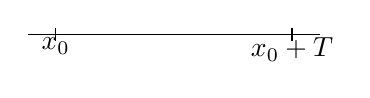
\begin{tikzpicture}
\draw (-0.35,0)--(3.35,0);
\draw (0,-0.08)--(0,0.08) node[below] {$x_0$};
\draw (3,-0.08)--(3,0.08) node[below] {$x_0+T$};
\end{tikzpicture}
\end{adjustbox}
Рассм. $y(x_0,x)$, $Ly=\lambda y$, $\lambda=k^2$.
\begin{equation*}
y|_{x=x_0}=1,\qquad y'|_{x=x_0}=ik.
\end{equation*}
— одна соб. ф-я (ближе к $e^{ikx}$).
\Incomplete{GELFAND-P000539}{monodromy-old}{Перед «и» отдельная старая запись покрыта пересекающимися зачёркиваниями; её содержание не восстановлено.}
и $\bar y(x_0,x)$ — другая соб. ф-я.
\underline{Матр. монодромии}
\begin{equation*}
y(x_0,x+T)=ay(x_0,x)+b\bar y(x_0,x),
\end{equation*}
причём $a=a(x_0,\lambda)$.
(обычн. матр. перех. [вписано над «перех.»: рассеяния] — за $\infty$ период — трив. вырожд. случай!)
\begin{equation*}
\bar y(x_0,x+T)=\bar b y(x_0,x)+\bar a\bar y(x_0,x).
\end{equation*}
\begin{equation*}
T=\begin{pmatrix}a&b\\\bar b&\bar a\end{pmatrix}
\text{ — матр. монодромии},\qquad T=T(x_0,\lambda).
\end{equation*}
$\det=1$ (Вронскиан постоянен).
\begin{gather*}
|a|^2-|b|^2=1;\\
SpT=2a_R=a+\bar a;\\
\text{Соб. числа }\alpha_\pm(\lambda)=a_R\pm\sqrt{a_R^2-1}.
\end{gather*}
рассм. график по $\lambda$.
[Слева горизонтальная линия; под левым концом λ.]
\begin{gather*}
\text{огр. решения}\Longleftrightarrow|a_R|\le1\Longrightarrow\text{получ. }e^{\pm it}\\
\text{неогр. решения}\Longleftrightarrow|a_R|>1\Longrightarrow\text{получ. }e^{\pm t}.
\end{gather*}

\SourcePage{GELFAND-P000540}{unlabelled}
$(y,y')=(1,ik)$.
\underline{Связь со спектром.}
\Unclear{GELFAND-P000540}{top-mark}{Перед «При» отдельный плотный вертикальный знак с двумя нижними окончаниями; возможное восклицательное выделение не утверждается.}
При $|a_R|\le1$ есть блоховский спектр.
\SourceFigure{GELFAND-P000540}{graph}{Справа график с подписью aR(λ), вертикальной осью и тремя почти горизонтальными линиями. Верхняя подписана 1, нижняя −1, средняя направлена вправо стрелкой с λ. Кривая слева спускается через 1, опускается ниже −1, поднимается выше 1 и вновь спускается ниже −1. Две прямоугольные полосы от верхнего до нижнего уровня заштрихованы. На средней оси справа и на верхней части кривой утолщения. Численные координаты и точное положение краёв полос в рисунке не заданы.}
Экспоненц. вне полосы. (в зоне монотонно).

\underline{Г.} $u(x)=const$ — спектр $>0$.
$u(x)<0$ может быть — зоны устойчивости залез. в отриц. обл.
\SourceFigure{GELFAND-P000540}{negative-sketch}{Справа короткая вертикальная линия от нижней горизонтали к верхнему заштрихованному овалу. Между ними две части горизонтального штриха с промежутком у вертикали. У нижнего пересечения чёрная точка и завитой знак, похожий на буквенную подпись; чтение знака и назначение уровней не установлены.}
\begin{equation*}
-y''+(a+b\cos2x)y=0.
\end{equation*}
зоны устойчив. и неустойч.
1-я зона уст. при $a+b\cos2x<0$.
(не быв. при постоянных).

\underline{Н.} может в зоне — одноз. для малых потенциалов.
\underline{Г. Конкурс на док-во} (к следующему разу).
\underline{Н.} Периодич. и антипериодич. $|a_R|=1$ — границы зон.
\SourceFigure{GELFAND-P000540}{double-sketch}{Слева вертикаль пересекает три горизонтальных уровня; средний со стрелкой вправо. Над средним выпуклая дуга касается верхнего уровня утолщённой вершиной. Сверху стрелка влево от подписи «вырожд. зона (соотв. 2-кр. выр.)». Масштаб, значения уровней и точная связь конца стрелки с вершиной не установлены.}
У пост. или 0-го всегда так:
\begin{equation*}
\begin{pmatrix}e^{iT}&0\\0&e^{-iT}\end{pmatrix},\qquad a_R=\cos T.
\end{equation*}

\underline{Об обр. задачах:} $a_R(k)=a_R(x_0,k)$ не определяет потенциал
\Incomplete{GELFAND-P000540}{inverse-old}{После «потенциал» внутри скобок в старой зачёркнутой записи различимы или-наоб…-подобные частичные следы; закрытые внутренние буквы и целая запись не восстановлены.}
($\approx$ информ. о спектре).

1) невырожд. $\lambda_n$: $b(x_0,\lambda)\ne0$.

2) \Unclear{GELFAND-P000540}{double-overwrite}{Перед читаемым «2-вырожд.» отдельный переписанный тёмный знак; старое чтение не установлено.}
2-вырожд. $\lambda_n$: $b(x_0,\lambda_n)\equiv0$.

Какие данные расс. опр. $u(x)$ \{кроме спектра\}.
Занимается Дубровин и уч. Фаддеева.
Если с нек-рого номера $\forall$ соб. т. 2-кр. вырожд., то запрещ. зоны стян. в точку.

\underline{Теорема.}
1) Рассм. $\sum_{i=0}^nQ_i(u,\ldots,u^{(k_i)})\frac{d^i}{dx^i}$ и пусть
\begin{equation*}
[A,L]=P(u,\ldots,u^{(\ell)})\qquad(\text{опер. умножения})
\end{equation*}
и рассм. диффер. ур-е $P(u,\ldots,u^{(\ell)})=0$ и пусть она периодич.
Тогда она — конечнозонный потенциал.
[Зачёркнуто:] или наоборот.
(На самом деле, верно и обратное).
\SourcePage{GELFAND-P000541}{60}
их по $1$ любого нечётного порядка.
(и любая лин. комбинация)

2) Все они — гамильт. сист. с $n$ степ. свободы.

\underline{Вопрос Н.: любой ли потенциал аппроксим. конечнозонными?}
\begin{equation*}
P_0=u',\qquad P_1=6uu'-u'''+cu',\ldots
\end{equation*}
2) $\exists$ матрица $2$-го порядка
\begin{equation*}
\Lambda(u,\ldots,u^{(k)},\delta)=
\begin{pmatrix}\lambda&\mu\\\bar\mu&\bar\lambda\end{pmatrix},
\qquad \lambda+\bar\lambda=0,
\end{equation*}
полином степ. $2k+1$ по $\delta$.
И другая матрица
\begin{equation*}
Q(u,\delta)=i\delta\begin{pmatrix}1&0\\0&-1\end{pmatrix}
-\frac{iu}{2\delta}\begin{pmatrix}1&-1\\1&-1\end{pmatrix},
\end{equation*}
такая что $P(u,\ldots,u^{(2k+1)})=0$ эквив. ур-ю $\Lambda'=[\Lambda,Q]$.
(в частн., соб. числа $\Lambda$ — интегралы ур-я)
\begin{equation*}
\Unclear{GELFAND-P000541}{spectral-alpha}{\alpha}_{\pm}(\delta)=\pm\sqrt{\det\Lambda}
\end{equation*}
— полином от $\delta$.
Коммутативн. интегралы — max набор.

Рассм. соб. ф-ю:
\begin{equation*}
\psi_k=e^{ikx}\ \ReaderApparatusRef{1}{2}
+\int_{-\infty}^{x}\chi(x,k)\,dx,\qquad L\psi=k^2\psi.
\end{equation*}
и (поправка к фазе $\int_{-\infty}^{x}\chi(x,k)\,dx$).
$I=\int\chi(x,k)\,dx$ сохр.
\begin{equation*}
\chi(x,k)=\sum_{n\ge1}\frac{\chi_n(x)}{k^n},\qquad
\chi_n(x)\text{ — полином},
\qquad I_n=\int_{-\infty}^{\infty}\chi_n(x)\,dx
\end{equation*}
как ф-я от $u$ — инт. ур-я К. д. Ф.

Пусть $(*)$ $\dot u=[A,L]$ — оп. ур-ие;
\Incomplete{GELFAND-P000541}{dotu-cancel}{Зачёркнутое слово перед обозначением L не читается.}
$L$ — опер. Штурма—Лиувилля.
$\psi_k$ — его соб. ф-я (эволюция $\psi_k$ — по потенциалу $u$).
\begin{equation*}
\dot\psi_k=A\psi_k+\lambda\psi_k+\mu\bar\psi_k,\qquad
\Lambda=\begin{pmatrix}\lambda&\mu\\\bar\mu&\bar\lambda\end{pmatrix}.
\end{equation*}
(хвост временной завис. соб. ф-й; начальная буква «х» переписана).
Применим $d/dx$ — получ. ур-е. $\psi_k(x_0,x)$.
При $x=x_0$ $(1,ik)$.
\begin{equation*}
\dot T=[\Lambda,T]
\end{equation*}
— эволюция матр. монодромии $T$.
\textit{Справа на поле: Теор. Новикова.}
\begin{equation*}
\frac{dT}{dx_0}=[Q,T],\qquad Q\text{ — станд. матрица (ур. для 2-курса)},
\qquad \Lambda'=[\Lambda,Q].
\end{equation*}
Границы зон — корни многочлена. (для стац. реш.)

\textit{Под нижней чертой:}
\Unclear{GELFAND-P000541}{bottom-authors}{Якубович}, Старжинский:
«Дифф. ур-я с периодич. коэффициентами».


\ReaderNotesStart{GELFAND-P000541}
\ReaderNote{1}{\Incomplete{GELFAND-P000541}{psi-cancellation}{Зачёркнутый фрагмент после экспоненты не читается.}}
\ReaderNotesEnd
\SourcePage{GELFAND-P000542}{unlabelled}
\underline{4/III–73. Сем. Гельфанда. Захаров В.}

Г. $L=-d^2/dx^2+u(x)$. Тогда $\exists$ опер. $A_n$,
$[A_n,L]=$ умн. на ф-ю $\Unclear{GELFAND-P000542}{flow-letter}{v}$,
$v=P_n(u,u',\ldots,u^{(n)})$.
\begin{equation*}
A_n=\frac{d^{2n+1}}{dx^{2n+1}}+\ldots\quad\text{(мл. члены)}.
\end{equation*}
Как найти $A_n$? Как связаны $A_n$ и $P_n$?
Отношение к ф-ле следов? Другие ур-я?

3. Результаты А. Б. Шабата и Захарова.

Пусть $F(x,y)$ сумм., $\int_{x_0}^{\infty}F(x,y)\,dy<C$ равномерно.
Гельф.—Левит. ур-е:
\begin{equation*}
K(x,y)+F(x,y)+\int_x^\infty K(x,s)F(s,y)\,ds=0.\qquad(1)
\end{equation*}
$x$ — параметр. Будем рассм. их как ядра оп.
\begin{equation*}
1+\hat F=(1+\hat K_+)^{-1}(1+\hat K_-),
\end{equation*}
$\hat K_{\pm}$ — вольтерровы.
$K_+(x,y)=0$ при $y<x$; $K_-(x,y)=0$ при $y>x$.
Это то же самое, $K+F+K*F=0$ — запись (1).

Дифференцируем по $t$ (параметр):
\begin{equation*}
D_tK+D_tF+D_tK*F+K*D_tF=0.\qquad(2)
\end{equation*}
Пусть $D$ и $\tilde D$ другие операторы:
$D$ действ. на $F$, $\tilde D$ действ. на $K$.
Ищем, чтобы
\begin{equation*}
\tilde DK+DF+\tilde DK*F+K*DF=0.\qquad(3)
\end{equation*}
Пусть $DF=\partial F/\partial x+\partial F/\partial y$,
$\tilde DK=\partial K/\partial x+\partial K/\partial y$.
Тогда всё в порядке (прямое вычисление показ., что вып. тожд. (3)).
\begin{equation*}
DF=\frac{\partial^n}{\partial x^n}F
\Unclear{GELFAND-P000542}{higher-df-sign}{\text{нечитаемый знак}}\ 
(-1)^n\frac{\partial^n\Unclear{GELFAND-P000542}{higher-df-overwrite}{\text{переписанный знак}}}{\partial y^n}F.\qquad(4)
\end{equation*}
Для него можно построить $\tilde D$.
$DF=[D_n,F]$, точнее $DF=$ ядро $[\hat D_n,\hat F]$,
где $\hat D_n=\partial^n/\partial x^n$.
Именно
\begin{equation*}
\tilde DK=L_nK+(-1)^n\frac{\partial^n}{\partial y^n}K.\qquad(5)
\end{equation*}
Г. $\partial^2K/\partial x^2-\partial^2K/\partial y^2=[\hat K,d^2/dx^2]$.
\textit{Над левой частью проведена дуга.}
Где $L_n=\partial^n/\partial x^n+\ldots$ (мл. члены).
$K,F$ могут быть и матрицами.

\SourcePage{GELFAND-P000543}{61}
\begin{equation*}
L_n=\frac{\partial^n}{\partial x^n}
+n\underbrace{\left(\frac d{dx}K(x,x)\right)}_{u_0(x)}
\frac{\partial^{n-2}}{\partial x^{n-2}}+\ldots\qquad(6)
\end{equation*}
Для мл. членов есть рекурр. ф-лы.
$L_n$ — нелинейный оператор от $K$, но его коэфф. (все)
сост. из величин $\xi_n(x)=(\partial/\partial x-\partial/\partial y)^nK|_{y=x}$.
$u_0=d\xi_0/dx$.
Коэфф. эти постоянны (при них).
Это не все операторы, дифферен. эту свертку.
Эти $D$ — линейные опер. с пост. коэфф. Можно и переменные.
Это алгебра Ли (
\Incomplete{GELFAND-P000543}{lie-cancel}{Зачёркнутый фрагмент после открывающей скобки не читается.}
все $D$, к-рые можно достроить (А. Шабат) — они описаны).

Предположим, что (1) однозначно разрешимо отн. $K$ ($F$ дано).
И пусть $F$ таково, что $\exists D:DF=0$. Отсюда
$\tilde DK=0$ (7) (из (2) и однозн. разреш. ур-я).
Отсюда $DF=0\Longleftrightarrow\tilde DK=0$ (8).
Получ. нек-рые линеаризующиеся ур-я. Но они неинтересны.

Пусть $D_1F=0$ и $D_2F=0$ (9).
\Unclear{GELFAND-P000543}{parameters-cancel}{Зачёркнуто: где}
даны $2$ параметры $t,z$; $F=F(x,y;t,z)$ и
\begin{align*}
D_1F&=\alpha\frac{\partial F}{\partial t}
+([\hat L_0^{(1)},\hat F])_{\text{ядро}},\qquad(10)\\
D_2F&=\beta\frac{\partial F}{\partial z}
+([\hat L_0^{(2)},\hat F])_{\text{ядро}},\qquad(11)
\end{align*}
$\hat L_0^{(1,2)}=\sum C^{(n)}\partial^n/\partial x^n$.
\begin{equation*}
\tilde D_1K=\alpha\frac{\partial K}{\partial t}
+L^{(\Unclear{GELFAND-P000543}{eq12-index}{i})}K
\Unclear{GELFAND-P000543}{eq12-sign}{\text{нечитаемый знак}}\ 
L_{0y}^{(1)t}K(x,y).\qquad(12)
\end{equation*}
$[\hat L^{(1)},\hat F]=L_x^{(1)}F-L_y^{(1)t}F$.
\begin{equation*}
\tilde D_2K=\beta\frac{\partial K}{\partial z}
+L^{(2)}K-L_{0y}^{(2)}K.\qquad(13)
\end{equation*}
$D_1F=0,\ D_2F=0\Longrightarrow\tilde D_1K=0,\ \tilde D_2K=0$ (14).
\underline{Теорема.}
\begin{equation*}
\beta\frac{\partial L^{(1)}}{\partial z}
-\alpha\frac{\partial L^{(2)}}{\partial t}
=[L^{(1)},L^{(2)}].\qquad(15)
\end{equation*}
$L^{(1)},L^{(2)}$ — лин. операторы (при заданном $K$).
В $L^{(1)}$ и $L^{(2)}$ входят коэффици., выраж. через
$\xi_n(x)=(\partial/\partial x-\partial/\partial y)^nK(x,y)|_{y=x}$.

\SourcePage{GELFAND-P000544}{unlabelled}
Это сист. нелин. д. у. отн. $\xi_n(x,\Unclear{GELFAND-P000544}{top-y-cancel}{\text{зачёркнуто }y},t,z)$.
\Incomplete{GELFAND-P000544}{top-cancel}{Зачёркнутое слово справа от первой строки не читается.}
Сист. для $K$ свод. к сист. для $F$ с пом. ур-я Г.—Л.
\Unclear{GELFAND-P000544}{cancel-line}{Зачёркнуто: по $F$ строим $K\Rightarrow\xi_n$.}
\Incomplete{GELFAND-P000544}{cancel-line-tail}{Последний короткий зачёркнутый фрагмент этой строки не читается.}

\textit{Вписано сверху справа:}
Зад. пару Л. д. оп. с пост. коэф. $L_0^{(1)}$ и $L_0^{(2)}$,
по ним стр. сист. ур-й (15). Пусть $D_1F=D_2F=0$,
где $F=F(x,y;t,z)$.
По $F$ строим $K$, и по $K$ строим реш. системы.
Получ. решение системы.

1-е нетрив. — ур-е
\Unclear{GELFAND-P000544}{kp-name}{Каданцева—Петриашвили(?)}.
\begin{gather*}
L_0^{(1)}=\frac{\partial^2}{\partial x^2},
\qquad L_0^{(2)}=\frac{\partial^3}{\partial x^3}+\lambda\frac{\partial}{\partial x},\\
L^{(1)}=\Unclear{GELFAND-P000544}{operator-overwrites}{\frac{\partial^2}{\partial x^2}}+u(x),
\qquad u(x)=2\frac d{dx}K(x,x),\\
L^{(2)}=\frac{\partial^3}{\partial x^3}
+\frac34\left(u\frac{\partial}{\partial x}+\frac{\partial}{\partial x}u\right)
+\lambda\frac{\partial}{\partial x}+w,\\
w=\frac32\frac d{dx}(\xi_1+\xi_0^2),\qquad
\xi_0=K(x,x),\qquad \xi_1=\left(\frac{\partial}{\partial x}-\frac{\partial}{\partial y}\right)K(x,y)|_{y=x}.
\end{gather*}
\textit{Числитель и знаменатель ведущего члена второго оператора также переписаны.}
(\Unclear{GELFAND-P000544}{xi-aside}{пр. по частям})
\begin{equation*}
\left\{\begin{aligned}
\frac34\beta\frac{\partial u}{\partial\Unclear{GELFAND-P000544}{system-z}{z}}&=-\frac{\partial w}{\partial x};\\
\beta\frac{\partial w}{\partial y}
&=\frac14\left(u_{xxx}+\Unclear{GELFAND-P000544}{system-correction}{3}uu_x\right)
+\lambda u_x+\alpha\frac{\partial}{\partial t}u.
\end{aligned}\right.
\end{equation*}
\textit{Над вторым уравнением в пузыре добавлено:} $+3u_xu$.
$u$ может быть матричным $\begin{pmatrix}u_0&u_1\\0&u_0\end{pmatrix}$;
для $u_1$ получ. линеариз. ур-е для $u_0$.
Дальше мет. линеаризации.
$\beta$ вещ. или мнимое, $\lambda\ldots$ Все имеют физ. смысл.

\SourceFigure{GELFAND-P000544}{hump-figure}{Над горизонтальной линией со стрелками и подписью x нарисован невысокий горб; справа над его склоном точка с подписью z. Точная форма профиля и расположение точки относительно него оставлены по скану.}
Обтекание тонкого крыла при
\Unclear{GELFAND-P000544}{wing-phrase}{произв. по струне}.

КДФ — если не зависит от $z$.
\underline{Нелин. струны.}
\begin{equation*}
\frac{\partial}{\partial x}\left\{\alpha\frac{\partial u}{\partial t}
+6uu_x+u_{xxx}+\lambda u_x\right.=\frac34\beta^2\frac{\partial^2u}{\partial z^2}.
\end{equation*}
Среда с дисперсией звука и мелкая вода.
Книга \underline{\Unclear{GELFAND-P000544}{book-name}{Кар[переписано]мана}} — см. там выводы. (кн. о нелин. волнах)
\begin{gather*}
L_0^{(1)}=\ell_1\frac{\partial}{\partial x}
+\ell_2\frac{\partial}{\partial\Unclear{GELFAND-P000544}{bottom-operator}{y}},
\qquad[\ell_1,\ell_2]=0,\qquad \ell_i\text{ — матрицы (диагон.)},\\
L^{(1)}=\ell_1\frac{\partial}{\partial x}+[\ell_1,\xi_0],
\qquad L^{(2)}=\ell_2\frac{\partial}{\partial x}+[\ell_2,\xi_0],
\qquad \xi_0(x)=K(x,x),\quad K\text{ — матрица}.
\end{gather*}

\SourcePage{GELFAND-P000545}{62}
\begin{equation*}
\ell_1=\begin{pmatrix}a_1&&0\\&\ddots&\\0&&a_n\end{pmatrix},
\qquad
\ell_2=\begin{pmatrix}b_1&&0\\&\ddots&\\0&&b_n\end{pmatrix}.
\end{equation*}
1-я нетрив. возник. в матр. $3\times3$.
$\partial\xi/\partial t+\vec V\nabla\xi$.
$u_1=\xi_{13},\quad u_2=\xi_{12},\quad u_3=\xi_{23},\quad
\xi^{\Unclear{GELFAND-P000545}{adjoint-sign}{+}}=\xi$.
\begin{equation*}
\left\{\begin{aligned}
\frac{\partial u_1}{\partial t}+\vec V_1\nabla u_1&=i\lambda u_2u_3;\\
\frac{\partial u_2}{\partial t}+\vec V_2\nabla u_2&=i\lambda u_1u_3^*;\\
\frac{\partial u_3}{\partial t}+\vec V_3\nabla u_3&=i\lambda u_1u_{\Unclear{GELFAND-P000545}{third-u}{2}}^*.
\end{aligned}\right.
\end{equation*}
$u_i(t,x,z)$, $\nabla$ — $2$-мерное, $\vec V_i$ — произв. вектора.
Опис. взаимод. волн $3$-х типов в нелин. среде.
\underline{Нельзя ввести диссипацию (никогда).}

Гипотеза: все они гамильтоновы, причем по одному $L$ стр. симплектич. форма,
а по другому — гамильтониан.
$u_{tt}-u_{xx}=\sin u$ тоже получается из матриц:
\SourceFigure{GELFAND-P000545}{matrix-l02}{Эскиз с подписью L нулевое верхний индекс 2: вертикальные ограничители матрицы, по диагонали сверху 1, -1, 0, 0; в правом верхнем и левом нижнем блоках большие 0. Пустые позиции и границы блоков не достраиваются.}
\SourceFigure{GELFAND-P000545}{matrix-l01}{Эскиз с подписью L нулевое верхний индекс 1: вертикальные ограничители матрицы, по диагонали сверху 1, 1, -1, -1; в правом верхнем и левом нижнем блоках большие 0. Пустые позиции и границы блоков не достраиваются.}
И ур-е о распр. лазерного импульса в…
Ур-е Блоха для матриц плотности (кв. мех. в $2$-уровн. системе).
Матр. опер. высоких порядков.
$L_0^{(1)}=\ell_1\partial_x,\quad L_0^{(2)}=\partial^2/\partial x^2$.
Получается
\begin{equation*}
i\frac{\partial\xi}{\partial t}+\xi_{xx}\pm|\xi|^2\xi=0
\qquad\text{(нелин. ур-е Шредингера)}.
\end{equation*}
Есть схема реш. зад. Коши.

\SourcePage{GELFAND-P000546}{unlabelled}
\underline{11/III–74. Сем. Гельфанда.}
Повзнер. \underline{Witham.}
\Incomplete{GELFAND-P000546}{speaker-heading-cancel}{Зачёркнутый фрагмент под фамилией докладчика не читается.}
\begin{equation*}
\frac{\partial^2u}{\partial t^2}-\frac{\partial^2u}{\partial x^2}+T'(u)=0.
\end{equation*}
\textit{Знаменатель первого члена переписан.}
1) бежит волна $x\sim t$ (практич. техника).
И асимпт. то, что происх. далеко:
$x\to x/\epsilon,\quad t\to t/\epsilon$.
Асимпт. ищется уже в конечной области и при $\epsilon\to0$.
$f(x-vt)$, $v$ мало зависит от $t$ и $x$ (медленно т. е. в смысле $\epsilon$).
Метод сост. в следующем:
\begin{equation*}
\epsilon^2\left(\frac{\partial^2v}{\partial t^2}
-\frac{\partial^2v}{\partial x^2}\right)+T'(u)=0.
\end{equation*}
Изуч. асимпт. в конечной области.
Доб. предположение (оправд. опытом науки):
\begin{equation*}
u(x,t)=f\left(\frac{\Theta_0(x,t)}{\epsilon};x,t\right).
\end{equation*}
$f(x_{\Unclear{GELFAND-P000546}{old-coordinate}{\text{ст}}}-ct_{\text{ст}})
=f((x-ct)/\epsilon)$ — точные бег. волны — частн. случай с $\Theta_0(x,t)=x-ct$.
$\Theta_0(x,t)/\epsilon=\Theta$; $f(\Theta;x,t)$.
Отсюда получается дифф. ур-е
\begin{equation*}
\epsilon^2(\omega_2^2-\omega_1^2)
\frac{\partial^2\Unclear{GELFAND-P000546}{expanded-u}{u}}{\partial\Theta^2}
+T'(u)\Unclear{GELFAND-P000546}{expanded-extra-mark}{u}
+[\epsilon(u_x,u_t)\ldots]=0,
\end{equation*}
где $\omega_2=\Theta_{0t},\quad\omega_1=\Theta_{0x}$.
При $\epsilon\to0$ получается
\begin{equation*}
\epsilon^2(\omega_2^2-\omega_1^2)\frac{\partial^2u}{\partial\Theta^2}+T'(u)=0,
\end{equation*}
обычн. ур-е $2$-го пор., $E_1,E_2$ — произв. пост.
$u=u(E_1,E_2;x,t,\Theta)$.
Уравнение для $\Theta$.
Теперь подставим $\Theta=\Theta_0(x,t)/\epsilon$.
\begin{equation*}
u=u\left(E_1,E_2;
\frac{\Theta_0(x,t)}
{\sqrt{\omega_2^2-\omega_1^2}\cdot
\Unclear{GELFAND-P000546}{action-symbol}{\psi}(E)\cdot\epsilon}\right).
\end{equation*}
(решение получ. в таком виде).
Доб. ур-е:
\Unclear{GELFAND-P000546}{additional-cancel}{Зачёркнуто: $\Theta_0/\theta_0$-подобный знак; прежние штрихи частично перекрыты.}
\begin{equation*}
\sqrt{\omega_2^2-\omega_1^2}\,
\Unclear{GELFAND-P000546}{action-symbol}{\psi}(E_1,E_2)=\mathrm{const},
\qquad
\Unclear{GELFAND-P000546}{action-symbol}{\psi}
=\int_{u_0}^{u_1}\sqrt{E-T(u)}\,du.
\end{equation*}
Лит.: Witham. Это ур-е, Кортевег, тяж. жидкость, радиофиз., лазеры.
J. of Fluid Mechanics. 1972. «Two-timing…» (Witham).

\SourcePage{GELFAND-P000547}{66}
\underline{В. Н. Туловский. О раб. Хёрмандера. Волновые фронты.}
$u\in\mathcal D'(\Omega),\quad\Omega\subset R^n$.
$(x_0,\xi_0)\notin WF(u)$, если $\exists\varphi\in C_0^\infty(\Omega)$,
$\varphi(x_0)\ne0$,
\begin{equation*}
|\langle u,\varphi e^{-i\langle x,\xi\rangle}\rangle|
\le C_N(1+|\xi|)^{-N}
\end{equation*}
в малой конич. окрестности точки $\xi_0$:
$|\xi/|\xi|-\xi_0/|\xi_0||<\epsilon$.

Примеры:
\SourceFigure{GELFAND-P000547}{step-example}{Слева короткий горизонтальный штрих с 1 над ним и 0 под ним; справа 1 обведена кружком, рядом 0 и стрелка к слову сверт. Не добавлены оси или отсутствующая ветвь графика.}
нормали; сверт. с $\delta$-обр. послед. и перех. к пред.
Г. $\int\varphi(x_1,x_2)e^{i(x_1\xi_1+x_2\xi_2)}\,dx_1\,dx_2$.
Стац. инт. по плоск. $\int\psi(t)e^{it}\,dt$.
\SourceFigure{GELFAND-P000547}{circle-oblique}{Окружность с тремя близкими наклонными параллельными штрихами возле правой стороны и тёмным пятном у контура. Подпись рядом: здесь будет особ. у ф-и $\psi(t)$. Точное касание штрихов к окружности не восстанавливается.}
\SourceFigure{GELFAND-P000547}{circle-horizontal}{Окружность с тремя близкими горизонтальными штрихами у нижней части и тёмным пятном справа внизу у контура. Подпись справа: особенности $\psi(t)$ нет. Точное положение штрихов относительно контура оставлено по скану.}
Тул. $\pi WF(u)=\operatorname{sing\,supp}u,\quad\pi(x,\xi)=x$.

$P:C_0^\infty(\Omega)\to C^\infty(\Omega_1)$,
$\exists K_P\in\mathcal D'(\Omega\times\Omega_1)$,
$\langle K_P,u(x)v(y)\rangle=\langle Pu,v\rangle$.
$WF(K_P)\overset{\text{def}}=WF(P)$.
В пр-ве $(x,y,\xi,\eta)$.
Пусть $WF(P)$ не содержит точек, где $\xi=0$ или $\eta=0$:
\fbox{$WF(P)\cap(\{\xi=0\}\cup\{\eta=0\})=\varnothing$}.
Тогда можно прод. $P:\mathcal E'(\Omega)\to\mathcal D'(\Omega_1)$.

Опред.
$WF'(P)=\{(x,y,\xi,\eta):(x,y,\xi,-\eta)\in WF(P)\}$.
Опред.
\begin{equation*}
WF'(P)\circ WF(u)=
\{(y,\eta):\exists(x,y,\xi,\eta)\in WF'(P),(x,\xi)\in WF(u)\}.
\end{equation*}
Теорема $WF(Pu)\subset WF'(P)\circ WF(u)$.
Пусть есть $2$ оператора:
\begin{gather*}
Q:\mathcal E'(\Omega_1)_y\to\mathcal D'(\Omega_2)_z,\qquad
P:\mathcal E'(\Omega)_x\to\mathcal E'(\Omega_1)_y,\\
WF'(Q\circ P)\subseteq WF'(P)\circ WF'(Q).
\end{gather*}
$(x,\Unclear{GELFAND-P000547}{bottom-z}{z};\xi,\zeta)\in WF'(P)\circ WF'(Q)
\underset{\text{def}}{\Longleftrightarrow}\exists(x,y,\xi,\eta)\in WF'(P),(y,z,\eta,\zeta)\in WF'(Q)$.

\SourcePage{GELFAND-P000548}{unlabelled}
\underline{Произведение обобщ. ф-й.}
$\Gamma\subseteq T^*(\Omega)\setminus0$, $\Gamma$ — конич. замкн. мн-во.
$\mathcal D_\Gamma(\Omega)=\{u\in\mathcal D'(\Omega),WF(u)\subseteq\Gamma\}$.
Теорема: пусть $\Gamma_1,\Gamma_2$ — $2$ замкн. конич. мн-ва в
$T^*(\Omega)\setminus0$ и пусть $\Gamma_1+\Gamma_2\subseteq\Omega\times(R^n\setminus0)$.
$(x,\xi)$, $(x,\eta)$; $\Gamma_1+\Gamma_2=\{(x,\xi+\eta)\}$, $\xi+\eta\ne0$.
Тогда сущ. непр. отобр.
\begin{equation*}
\mathcal D_{\Gamma_1}(\Omega)\times\mathcal D_{\Gamma_2}(\Omega)
\longrightarrow\mathcal D_{\Gamma_1\cup\Gamma_2\cup(\Gamma_1+\Gamma_2)}(\Omega),
\end{equation*}
продолжающее произвед. обычных ф-й.
(и произв. обобщ. ф-и на гладкую)
(Оно единственно из-за рассм. топологии)

\underline{Опр. интегр. опер. Фурье.}
$\varphi(x,\Theta)$, $(x,\Theta)\in\Omega\times(R^N\setminus0)$ —
фаз. ф-я, если она веществ., однородна $1$-го пор. \textit{(вписано: по $\Theta$)}
и $\varphi'_{x,\Theta}\ne0$.
\begin{equation*}
S_{\rho,\delta}^m(X\times R^N)\ni a(x,\Theta),\qquad
|\partial_x^\alpha\partial_\Theta^\beta a(x,\Theta)|
\le C_{\alpha,\beta}(1+|\Theta|)^{m-\rho|\beta|+\delta|\alpha|},
\quad x\in K.
\end{equation*}
\textit{В последнем условии x переписано.}
\begin{align*}
\langle A,u\rangle&=\int e^{i\varphi(x,\Theta)}a(x,\Theta)u(x)\,dx\,d\Theta\\
&=\lim_{\epsilon\to0}\int e^{i\varphi(x,\Theta)}
a(x,\Theta)\chi(\epsilon\Theta)u(x)\,dx\,d\Theta,
\end{align*}
где $\chi\in C_0^\infty(R^N)$, $\chi=1$ при $|\Theta|<1$.

\SourcePage{GELFAND-P000549}{unlabelled}
\underline{18/III–74. Сем. Гельфанда. А. Б. Шабат.}
\begin{equation*}
4f_t+f_{xxx}+ff_x=0,\qquad
f(x,t)=g(x-ct)=\frac{2\lambda^2}{\operatorname{ch}^2[\lambda(x-\lambda^2t-h)]}.
\end{equation*}
$2$-х солит. решение
\begin{equation*}
f(t,x)=\ldots^{\lambda_1}+\ldots^{\lambda_2}
+O(e^{-\Unclear{GELFAND-P000549}{big-o}{\alpha}t})
\quad\text{при }t\to+\infty.
\end{equation*}
Можно док., что оно единственно.
1) Оценить суммарную амплитуду в момент столкновения.
\begin{equation*}
|f(t,x)|\le2\sum_{j=0}\lambda_j(\lambda_{j+1}-\lambda_j),\qquad\lambda_0=0
\end{equation*}
(не склад. амплит. как в лин. случае).
2) Центры сместятся. Вычислить смещение. Ответ станд. — рассеяние.
Потенциал Баргмана $q(x)$, если $\exists2$ реш. ур-я
$y''+(q(x)+\xi^2)y=0$ вида
$y_{1,2}=P_{1,2}(x,\xi)e^{\mp i\xi x}$, многочлен по $\xi$.
\textit{На левом крае рядом с последними строками виден обрезанный фрагмент:}
\Incomplete{GELFAND-P000549}{left-cutoff}{На левом крае виден только конец соседней записи со знаком равенства; остальное вне кадра.}

\Unclear{GELFAND-P000549}{spectral-letter}{Спектральная буква в формулах этой страницы допускает $\xi/\zeta$; $\xi$ оставлено предварительно.}

\SourcePage{GELFAND-P000550}{unlabelled}
\textit{Слева на поле:} Пусть $P,Q$ — полиномы.
\begin{equation*}
c_ke^{2i\xi x}|_{\xi=\xi_k}=
\frac{P(x,\xi)}{Q(x,\xi)}|_{\xi=\xi_k},\qquad
\frac PQ|_{\xi=\infty}=1.
\end{equation*}
\textit{Справа на поле:} Точек $\xi_k$:
$2n\Unclear{GELFAND-P000550}{count-points}{\text{нечитаемый знак}}1$ (и $+\infty$).
При любом выборе параметров $c_k,\xi_k$ получ. фунд. сист. решений
опер. Ш.—Л. с потенц. Баргмана
$y_1=P(x,\xi)e^{i\xi x},\quad y_2=Q(x,\xi)e^{-i\xi x}$.
1. $P'_xQ-Q'_xP-2i\xi PQ=\prod(\xi-\xi_k)$.
Дифф. по $x$:
\begin{equation*}
\frac d{dx}\frac PQ|_{\xi=\xi_k}=
\frac{P'_xQ-Q'_xP}{Q^2}|_{\xi=\xi_k}=
2i\xi\frac PQ|_{\xi=\xi_k}
\end{equation*}
есть рац. ф-я по $\xi$ с $0$-ми в
\Incomplete{GELFAND-P000550}{canceled-word}{Зачёркнутое слово между «в» и «зад. точках» не читается.}
зад. точках
\begin{equation*}
\frac{P_xQ-Q_xP-2i\xi PQ}{Q^2}|_{\xi=\xi_k}=0.
\end{equation*}
И одно усл. на $\infty$.
Пусть теперь $c_k$ зависит от $t$ (параметра):
\begin{equation*}
c_k(\Unclear{GELFAND-P000550}{ck-t-overwrite}{t})=c_k(0)e^{2i\xi^3t},\qquad
\frac PQ|_{\xi=\xi_k}=c_k(t)e^{2i\xi x}|_{\xi=\xi_k}.
\end{equation*}
Тогда ещё
\begin{equation*}
\left(4\frac{\partial}{\partial t}+\frac{\partial^3}{\partial x^3}
-3q\frac{\partial}{\partial x}\right)P=
\Unclear{GELFAND-P000550}{empty-operator}{(\quad)}Q=0.
\end{equation*}
Тогда $f=\frac d{dx}\log Pe^{\Unclear{GELFAND-P000550}{log-sign}{\pm}i\xi x}$
удовл. $4f_t+f_{xxx}+3(f^2+\xi^2)f_x=0$,
а $f'+f^2=q$ удовлетвор. ур-ю $4q_t+q_{xxx}+6qq_x=0$.
\Unclear{GELFAND-P000550}{spectral-letter}{Спектральная буква в формулах этой страницы допускает $\xi/\zeta$; $\xi$ оставлено предварительно.}
\SourcePage{GELFAND-P000551}{unlabelled}
[Большая верхняя область кадра свободна; запись внизу.]
\underline{25/III−74. Сем. Гельфанда.}

\underline{Кириллов. О беск. группах.} Опис. предст. след. групп
\begin{equation*}
G_1=Diff\,M,\qquad G_2=H^M=C^\infty(M,H)\qquad(H\text{ — группа}).
\end{equation*}
\Unclear{GELFAND-P000551}{bundle-conjunction}{Слева от схемы отдельный знак с двумя высокими штрихами и нижним соединением; и/И или H-подобное чтение не установлено. Знак отличен от H рядом со стрелкой.}
\begin{adjustbox}{max width=\linewidth}
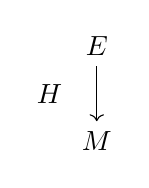
\begin{tikzpicture}
\node at (0,0.6) {$E$};
\node at (0,-0.6) {$M$};
\node at (-0.6,0) {$H$};
\draw[->] (0,0.35)--(0,-0.35);
\end{tikzpicture}
\end{adjustbox}
главное рассл. и группа его автоморфизмов.
Она проектир. на $G_1$ со слоем $G_2$.
\Incomplete{GELFAND-P000551}{bundle-old}{Под схемой расслоения прямоугольная старая запись покрыта плотными зачёркиваниями; её содержание целиком не восстановлено.}

\begin{equation*}
e^H=H_0\oplus H\oplus S^2(H)\oplus S^3(H)\oplus\ldots
\end{equation*}
\Unclear{GELFAND-P000551}{fock-upper-marks}{Над областями H/⊕ и S²(H) два отдельных горизонтальных штриха; между ними маленький завиток или точечный знак. Их точное прикрепление к слагаемым и математическое значение не установлены.}
($H_0$ — одномерное; $S^k(H)$ — симметр. степень
[Под первыми тремя слагаемыми:]
\begin{equation*}
1\qquad\xi\qquad\frac{\xi\otimes\xi}{2!}
\end{equation*}
\Unclear{GELFAND-P000551}{fock-product}{В степени два знак внутри овала имеет плотный диагональный штрих и короткий пересекающийся остаток; ⊗ передано предположительно.}
[Справа:]
\begin{equation*}
|\xi|^2=\sum\frac{|\xi_n|^2}{n!}.
\end{equation*}

\underline{Гуревич.} Об ур-
\Unclear{GELFAND-P000551}{gurevich-old}{После «ур-» переписанное короткое окончание с двумя плотными верхними штрихами и правым нижним крюком; «ие» возможно, но старые буквы не установлены.}
К-д-Ф. методом Уидема.

\SourcePage{GELFAND-P000552}{unlabelled}
\underline{1/IV−74. Сем. Гельфанда.}
\underline{Юра Кобленц. Об асимптотике соб. значений опер. Лапласа.}
[Вписано над следующей строкой:] (из Ленинграда)
$M$ — замкн. рим. мн-во. $\Delta$ — опер. Бельтрами—Лапласа.
\begin{gather*}
\lambda_0=0,\qquad0\le\lambda_1\le\lambda_2\le\ldots\text{ — спектр.}\\
Z(s)=Tr\exp(-s\Delta)=\sum e^{-\lambda_i s}.
\end{gather*}
\begin{equation*}
\Delta f=\frac1{\sqrt g}\frac{\partial}{\partial x^i}
\left(\sqrt g\,g^{ij}\frac{\partial f}{\partial x^j}\right),
\qquad\text{где }g=\det\Vert g_{ij}\Vert.
\end{equation*}
\Incomplete{GELFAND-P000552}{laplacian-old}{Между знаком равенства и читаемым 1/√g плотный вытянутый зачёркнутый блок целиком не восстановлен. Короткий выходящий правый штрих не отделён уверенно от зачёркивания; знак перед дробью не добавлен.}
\begin{equation*}
E(m,m',t)=\sum e^{-\lambda_i t}\varphi_i(m)\varphi_i(m').
\end{equation*}
\Unclear{GELFAND-P000552}{kernel-functions}{Оба знака перед индексами i имеют открытую левую ветвь, правую петлю и нижний штрих; второй плотнее. ϕ передано предположительно, чтение ψ не исключено. Черта сопряжения над вторым множителем не написана.}
\begin{equation*}
Z(s)=\int E(m,m,s)\,dm.
\end{equation*}
\underline{Minakshisundaram, 1949}
\begin{equation*}
Z(t)=(4\pi t)^{-n/2}(a_0+a_1t+a_2t^2+\ldots),
\qquad t\to0,\quad\Re t>0.
\end{equation*}
\begin{equation*}
n=\dim M,\qquad a_0=vol\,M,
\end{equation*}
\begin{equation*}
a_1=\int_M\frac\tau6\,dV,\qquad\text{где }\tau\text{ — скал. кривизна}.
\end{equation*}
[Справа:]
\begin{equation*}
\tau=\sum_{\alpha\beta\,\text{[переписано]}\,\beta}
R_{\alpha\beta\,\text{[зачёркнуто]}}^{\alpha\beta}.
\end{equation*}
\Unclear{GELFAND-P000552}{scalar-indices}{Под Σ видны слева α, β, далее плотные переписанные штрихи и справа β; у R верхние αβ и начало нижних αβ читаются, после них ещё два зачёркнутых знака. Полная старая последовательность индексов не установлена.}
\begin{equation*}
a_2=\frac1{360}\int\left(2|R|^2-2|\rho|^2+5\tau^2\right).
\end{equation*}
$R$ — тензор кривизны; $\rho$ — тензор Риччи,
\begin{equation*}
\rho_{ij}=\sum_\alpha R_{i\alpha j}^{\alpha}.
\end{equation*}
\Unclear{GELFAND-P000552}{ricci-indices}{После нижнего j у R отдельный плотный переписанный знак с пересекающимися штрихами. Последние старые штрихи не восстановлены; читаемые iαj и верхнее α переданы отдельно.}
\begin{equation*}
|R|^2=\sum R_{\alpha\beta\gamma\delta}^2,
\qquad\text{в норм. коорд. }|R|^2=R_{\alpha\beta\gamma\delta}R^{\alpha\beta\gamma\delta},
\end{equation*}
\begin{equation*}
|\rho|^2=\rho_{\alpha\beta}\rho^{\alpha\beta}.
\end{equation*}
\begin{equation*}
E(t,m,m')=(4\pi t)^{-n/2}
\left(u_0(m,m')+u_1(m,m')t+u_2(m,m')t^2+\ldots\right)
\end{equation*}
в окр. диагонали.
$a_3$ — Sakai и докладчик (независимо).

\underline{Г. Число цел. точек в круге:}
\begin{equation*}
a(r)=\pi r^2+\sum_{\lambda_n}\tau^{1/2}\sin\frac\tau{\lambda_n}.
\end{equation*}
\Unclear{GELFAND-P000552}{circle-formula}{В аргументе a и после π короткие верхние штрихи похожи на r или τ; r передано предположительно. В членах суммы длинная волнистая верхняя черта передана как τ. Единое обозначение редакционно не введено.}
($\lambda_n$ — нули $\zeta$-ф-и Римана.) mod гипотезу Римана.
[Слева на поле:] \underline{Шнирельман.}
В игре $\lambda_n$ — длины замкн. биллиардных путей.
\begin{equation*}
\sum\delta(\lambda-\lambda_k)*\frac\varepsilon{\lambda^2+\varepsilon^2}=f(\lambda).
\end{equation*}

\SourcePage{GELFAND-P000553}{83}
\begin{equation*}
f(\lambda)=f_0(\lambda)+\sum_k c_k\lambda^{\alpha_k}\sin(\ell_k\lambda+\omega_k).
\end{equation*}
Есть экспер. подтверждение (Balian и Bloch)
\Unclear{GELFAND-P000553}{balian-name}{После читаемого Balia последний знак плотный, с двумя высокими верхними штрихами и нижним правым крюком; n в Balian передано предположительно, более ранние штрихи не установлены.}
(и даже точное утверждение).
\begin{equation*}
\sum e^{i\lambda_k z}=Sp(e^{-z\Delta}).
\end{equation*}
\Unclear{GELFAND-P000553}{trace-exponent}{Слева перед λk написано i, справа показатель −zΔ без i. Оба показателя видны; равенство сохранено без согласования знаков и операторов.}
продолж. вниз (из верхн. полуплоск.)

\underline{Пробл. близнецов:}
\begin{equation*}
\lambda_{k+1}-\lambda_k>c\lambda_k^{-N}\quad\text{для общих операторов}.
\end{equation*}
Но на окружности двойные. (устойчиво асимпт. 2-кр. спектр).
[Слева на поле:] $T^2$.
$g_{ij}\sim\delta_{ij}$ — справ. теорема
\underline{Теорема.}
\begin{equation*}
\min(\lambda_{k+1}-\lambda_k,\lambda_k-\lambda_{k-1})<C_N k^{-N},\qquad\forall N.
\end{equation*}
(Лазуткин, Шнирельман)
\Unclear{GELFAND-P000553}{attribution}{Во второй фамилии после читаемого «Шнирель» средняя часть перед «ан» переписана плотнее; «Шнирельман» передано предположительно, старые буквы не установлены.}
(малое, но конечное возмущение) — устойч.
Для $T^3$ это уже не так. (по-видимому).

\begin{equation*}
\frac{\partial u}{\partial t}=i\sqrt{-\Delta}\,u;\qquad u|_{t=0}=\delta_x.
\end{equation*}
\Unclear{GELFAND-P000553}{wave-numerator}{В числителе после ∂ плотный переписанный знак с u-подобной верхней частью и чёрной нижней петлёй. u передано предположительно; прежний знак не установлен.}
Её реш. $u(x,y,t)$
\begin{equation*}
\sum e^{i\lambda_k t}=\int_M u(x,x,t)\,dx=f(t);
\end{equation*}
\Unclear{GELFAND-P000553}{trace-time}{Последний аргумент u на диагонали переписан: видны высокий штрих, поперечина и нижний крюк. t передано предположительно; более ранний знак не восстановлен.}
особ. $u(x,y,t)$ там, где $|x-y|=t$.
\SourceFigure{GELFAND-P000553}{loop}{Слева вертикальный штрих, на нём плотная точка, от которой вправо выходит замкнутая вытянутая петля. Стрелки и буквенные метки не написаны; назначение вертикали и точная геометрическая связь петли с соседним текстом не установлены.}
при нек. $t$ происх. бифуркации.
\Unclear{GELFAND-P000553}{bifurcation-ending}{После читаемого «бифуркаци» два плотных переписанных штриха с правым крюком; окончание «и» в переданном «бифуркации» предположительно, прежние буквы не установлены.}
Особ. движ. со скор. 1.

\end{document}
